\documentclass[french, 12pt]{article} % use larger type; default would be 10pt

\usepackage[utf8]{inputenc} % set input encoding (not needed with XeLaTeX)
\usepackage[T1]{fontenc}

%%% PAGE DIMENSIONS
\usepackage{geometry} % to change the page dimensions
\geometry{a4paper} % or letterpaper (US) or a5paper or....
% \geometry{margin=2in} % for example, change the margins to 2 inches all round

%PACKAGES
\usepackage{booktabs} % for much better looking tables
\usepackage{array} % for better arrays (eg matrices) in maths
\usepackage{paralist} % very flexible & customisable lists (eg. enumerate/itemize, etc.)
\usepackage{verbatim} % adds environment for commenting out blocks of text & for better verbatim
\usepackage{subfig} % make it possible to include more than one captioned figure/table in a single float
\usepackage{graphicx} % support the \includegraphics command and options
\usepackage[colorlinks=true]{hyperref} % permet l'utilisation d'hyperliens, et active leur coloration ( a definir)
\usepackage{pdfpages} %% permet d'importe des pages pdf
\usepackage[francais]{babel}

%GLOSSAIRE
%\usepackage{glossary}
\usepackage[toc]{glossaries}
\makeglossaries
\newacronym{AVC}{AVC}{accident vasculaire cérébral}

\newacronym{bat}{BAT}{bimanual arm training}

\newacronym{chac}{CHAC}{Centre Hospitalier Alès - Cévennes}

\newacronym{fps}{FPS}{First Person Shooter}

\newacronym{gui}{GUI}{graphical user interface}

\newacronym{ia}{IA}{intelligence artificielle}

\newacronym{imagina}{IMAGINA}{IMAges, Games and INtelligent Agents}

\newacronym{lirmm}{LIRMM}{Laboratoire d'Informatique, de Robotique et de Microélectronique de Montpellier}

\newacronym{m2h}{M2H}{Movement to Health Laboratory}

\newacronym{mig}{MIG}{Montpellier In Game}

\newacronym{mojos}{MoJOS}{Moteur de Jeux Orienté Santé}

\newacronym{mvc}{MVC}{Modèle-Vue-Contrôleur}

\newacronym{nui}{NUI}{natural user interface}

\newacronym{um2}{UM2}{Université Montpellier II}

\newacronym{rts}{RTS}{Real Time Strategy}

\newacronym{sg}{SG}{Serious Game}

\newglossaryentry{casual}{
	name={casual},
	description={Se dit d'une personne ne jouant à des jeux vidéo que de manière occasionnelle. Peut aussi se dire d'un jeu dont la cible sont des joueurs occasionnels}
}

\newglossaryentry{ergotherapie}{
	name={ergothérapie},
	description={L'ergothérapie est une profession de santé évaluant et traitant les personnes afin de préserver et développer leur indépendance et leur autonomie dans leur environnement quotidien et social}
}

\newglossaryentry{feedback}{
	name={feedback},
	description={retour d'information du jeu suite ou non à une action du joueur. 
Généralement : l’action en retour d’un effet sur le dispositif qui lui a donné naissance, et donc, ainsi, sur elle-même}
}

\newglossaryentry{fuglmeyer}{
	name={Fugl Meyer},
	description={Le test de Fugl Meyer est un ensemble d'exercices à réaliser permettant d'évaluer les capacités motrices d'une personne. Chaque exercice fournit un score dont l'évaluation totale permet d'estimer des progrès du patient}
}

\newglossaryentry{hardcore}{
	name={hardcore},
	description={Par opposition au jeu \gls{casual}, le jeu hardcore cible les très gros joueurs et possède un niveau de difficulté très élevé, demandant un fort investissement de la part du joueur. On appelle aussi ce type de joueurs des hardcore gamers}
}

\newglossaryentry{hemiplegie}{
	name={hémiplégie},
	description={Une hémiplégie est une paralysie d'un seul côté du corps. La paralysie peut affecter une ou plusieurs parties de l'hémicorps, jusqu'à être totale si la face, le tronc et les membres supérieurs et inférieurs sont paralysés}
}

\newglossaryentry{hypertonie}{
	name={hypertonie spastique},
	description={L’hypertonie spastique (musculaire) est une contraction réflexe du muscle qui s'oppose à l'étirement}
}

\newglossaryentry{lombalgie}{
	name={lombalgie},
	description={Une lombalgie est un état douloureux du rachis lombaire}
}

\newglossaryentry{paresie}{
	name={parésie},
	description={Perte partielle des capacités motrices d'une partie du corps (limitation de mouvement, diminution de la force musculaire), par opposition à la paralysie où le déficit moteur est total}
}

\newglossaryentry{serious gaming}{
	name={serious gaming},
	description={Dérivation de l'utilisation d'un jeu vidéo classique dans un but sérieux.}
}

\newglossaryentry{spasticite}{
	name={spasticité},
	description={La spasticité consiste en un étirement rapide d'un muscle qui entraîne trop facilement sa contraction réflexe qui dure un certain temps}
}

\newglossaryentry{skill}{
	name={skill},
	description={Technique ou compétence dans un jeu vidéo, peut représenter les actions possibles d'un personnage.}
}
%\newglossaryentry{}{
%	name={},
%	description={}
%}


%COULEURS
\usepackage{color} % permet de définir des couleurs pour les utiliser localement
\definecolor{orange}{rgb}{0.8, 0.4, 0.1}
\definecolor{vert}{rgb}{0.27, 0.57, 0.13}
\definecolor{marron}{rgb}{0.6, 0.2, 0.13}

% BIBLIOGRAPHY DEFINITIONS
\bibliographystyle{plain}


% HEADERS & FOOTERS
\usepackage{fancyhdr} % This should be set AFTER setting up the page geometry
\pagestyle{fancy} % options: empty , plain , fancy
\renewcommand{\headrulewidth}{0pt} % customise the layout...
\lhead{}\chead{}\rhead{}
\lfoot{}\cfoot{\thepage}\rfoot{}

% SECTION TITLE APPEARANCE
\usepackage{sectsty}
\allsectionsfont{\sffamily\mdseries\upshape} % (See the fntguide.pdf for font help)

% table of contents APPEARANCE
\usepackage[nottoc,notlof,notlot]{tocbibind} % Put the bibliography in the ToC
\usepackage[titles,subfigure]{tocloft} % Alter the style of the Table of Contents
\renewcommand{\cftsecfont}{\rmfamily\mdseries\upshape}
\renewcommand{\cftsecpagefont}{\rmfamily\mdseries\upshape} % No bold!


\title{Rapport de stage - M2 Informatique}
\author{Mélia Geoffrey}

\date{} % Activate to display a given date or no date (if empty), otherwise the current date is printed 

\ifpdf
	\pdfinfo
	{
		/Author (Geoffrey MELIA)
		/Title (Master thesis)
		/Subject (Difficulty adaptation in rehabilitation SG)
		/Keywords (serious games ; rehabilitation ; difficulty adaptation ; player behavior ; conception)
		/CreationDate (\today)
	}
\fi

\begin{document}
\maketitle

\begin{picture}(0,0)
	\put(-30,-550){
\includegraphics[scale=0.8]{images/logo_um2.png}}
	\put(280,-570){
\includegraphics[scale=0.6]{images/logo_naturalpad.png}}
	
	\put(-30,-120){\textsc{\LARGE{Vers une méthode de conception de jeux}}}
	\put(10,-150){\textsc{\LARGE{vidéo sérieux à but thérapeutique}}}
	\put(100,-180){\textsc{\large{et adaptation de la difficulté}}}
	
	\put(-30,-360){\textsc{\large{tuteurs universitaires : Vincent Boudet \& Nancy Rodriguez}}}
	\put(-30,-400){\textsc{\large{effectué chez la société NaturalPad}}}
	\put(-30,-420){\textsc{\large{sous la direction de Antoine Seilles}}}
\end{picture}

\newpage \newpage
\section*{Remerciements}
\addcontentsline{toc}{section}{Remerciements}
Je tiens tout d'abord à remercier Antoine Seilles pour avoir conçu et proposé un sujet de stage en accord à la fois avec les besoins de l'entreprise et mes affections, pour son aide avisée tout au long de ce stage ainsi que pour la confiance qu'il a mise en moi et en mon travail.

\paragraph{}Je remercie aussi Inès Di Loretto qui, malgré la distance, m'a apporté de manière régulière et amicale son aide, son expérience de chercheuse, ses idées et son regard critique sur mon travail, et a su me guider et me faire poser les bonnes questions.

\paragraph{}Merci à Sebastien Andary et Anthony Barreau pour avoir partagé leurs connaissances techniques et technologiques et contribué à améliorer mon travail. Merci aussi pour m'avoir soutenu et contribué au bon déroulement de mon stage.

\paragraph{}Je remercie Nancy Rodriguez pour son suivi et conseils sur mon travail, dont l'oeil critique était le bienvenu.

\paragraph{}Un grand merci à Didier Costeau\footnote{Kinésithérapeute, en libéral à Montpellier}, Karima Bahkti\footnote{Kinésithérapeute au centre hospitalier de Lapeyronie, Montpellier}, Julien Métro\footnote{PhD student au laboratoire Movement 2 Health}, Arnaud Dupeyron\footnote{Docteur en médecine spécialisé dans la lombalgie, EUROMOV, Movement 2 Health} et Anaïs Ivorra\footnote{Ergothérapeute} pour m'avoir accordé leur temps et partagé leur expérience et connaissances médicales, sans lesquelles aucun travail n'aurait été possible, et de manière générale à tous les professionnels de la santé impliqués dans ce projet.

\paragraph{}Merci enfin à toute l'équipe de NaturalPad et à Fabien Dutartre pour l'expérience humaine à laquelle ils m'ont fait participer durant ces six mois, quand travail et plaisir ne font plus qu'un.

\definecolor{red}{rgb}{0,0,0}
\newpage
\tableofcontents

\newpage
\listoffigures
\definecolor{red}{rgb}{1,0,0}

\newpage 

\part{Rapport de stage}
	\section{Introduction}
	\subsection{Généralité}	
Ce stage réalisé dans le cadre de ma 2$^{eme}$ année de Master Informatique fut l'occasion de poursuivre mon travail dans le domaine de la santé débuté durant mon TER. Succintement, ce travail consistait en l'expérimentation de l'utilisation de technologies informatiques pour l'évaluation des capacités motrices de patients hémiplégiques. Ce projet de TER a été réalisé avec William DYCE, par ailleurs stagiaire avec moi chez NaturalPad. Nous avons conçu un prototype d'application permettant, grâce à la Kinect, de juger de la réussite ou non de plusieurs des exercices d'évaluation du test de %\gls{fuglmeyer} 
par un patient en réhabilitation suite à un AVC. \paragraph{}
Fort de cette expérience et vivement motivé par le fait de travailler dans un contexte médical, ce stage constituait une excellente opportunité d'orienter ma formation vers le développement d'applications et de jeux pour la santé.\\
L'objectif de ce stage était de proposer un moyen ou des outils pour adapter la difficulté de jeux sérieux pour la santé dans le domaine de la rééducation motrice. Nous verrons que différentes approches sont possibles et quelle fut démarche lors de ce stage. Par ailleurs, ce fut pour moi l'occasion de m'insérer dans le projet de grande envergure, Hammer \& Planks, et de participer à mes deux premières GameJam, comme je le détaillerai en annexe.

\subsection{L'entreprise}
	\subsubsection{Naturalpad}
NaturalPad est une jeune startup innovante basée dans la région de Montpellier. Elle est spécialisée dans les technologies appliquées à la santé et développe notamment des jeux vidéos à but thérapeutique pour la rééducation fonctionnelle. Ces jeux utilisent des technologies de capture du mouvement grand public comme le Kinect de Microsoft ou la Wii Board de Nintendo. L’idée de Naturalpad est née lors du projet MoJOS (Moteur de Jeux Orienté Santé), pionnier en matière de projet de recherche serious game, sur lequel plusieurs membres de l’équipe ont travaillé. En effet, prenant conscience du marché porteur des serious games et plus largement de celui de la santé, Antoine Seilles et les 4 autres fondateurs ont créé le projet NaturalPad en se démarquant des concurrents par une volonté de faire avant tout du jeu, bien qu’il soit sérieux, et d’y apporter une dimension sociale. L’idée au delà du développement de jeux est de proposer un système sous forme de plateforme intégrant plusieurs jeux thérapeutiques. Ceux-ci permettant au patient de suivre sa thérapie à domicile tout en jouant avec ses proches (ils sont considérés dans la conception du gameplay) et donnant la possibilité au thérapeute de suivre la progression du patient. NaturalPad a par ailleurs signé un partenariat avec le Centre Hospitalier Alès Cévennes (CHAC) dans le but de développer des services web innovants pour les équipes de pédiatrie, néonatalogie et gériatrie du CHAC. Le CHAC peut être considéré comme le site pilote des produits NaturalPad. Un partenariat de recherche a été mis en place avec deux laboratoires de recherche de Montpellier que sont le LIRMM (Laboratoire d’Informatique, de Robotique et de Microélectronique de Montpellier) et le M2H (Movemement 2 Health : Laboratoire en Sciences du Mouvement) dans le cadre des activités de NaturalPad.

	\subsubsection{L'équipe}
	\begin{figure}[!h]
		\centering
		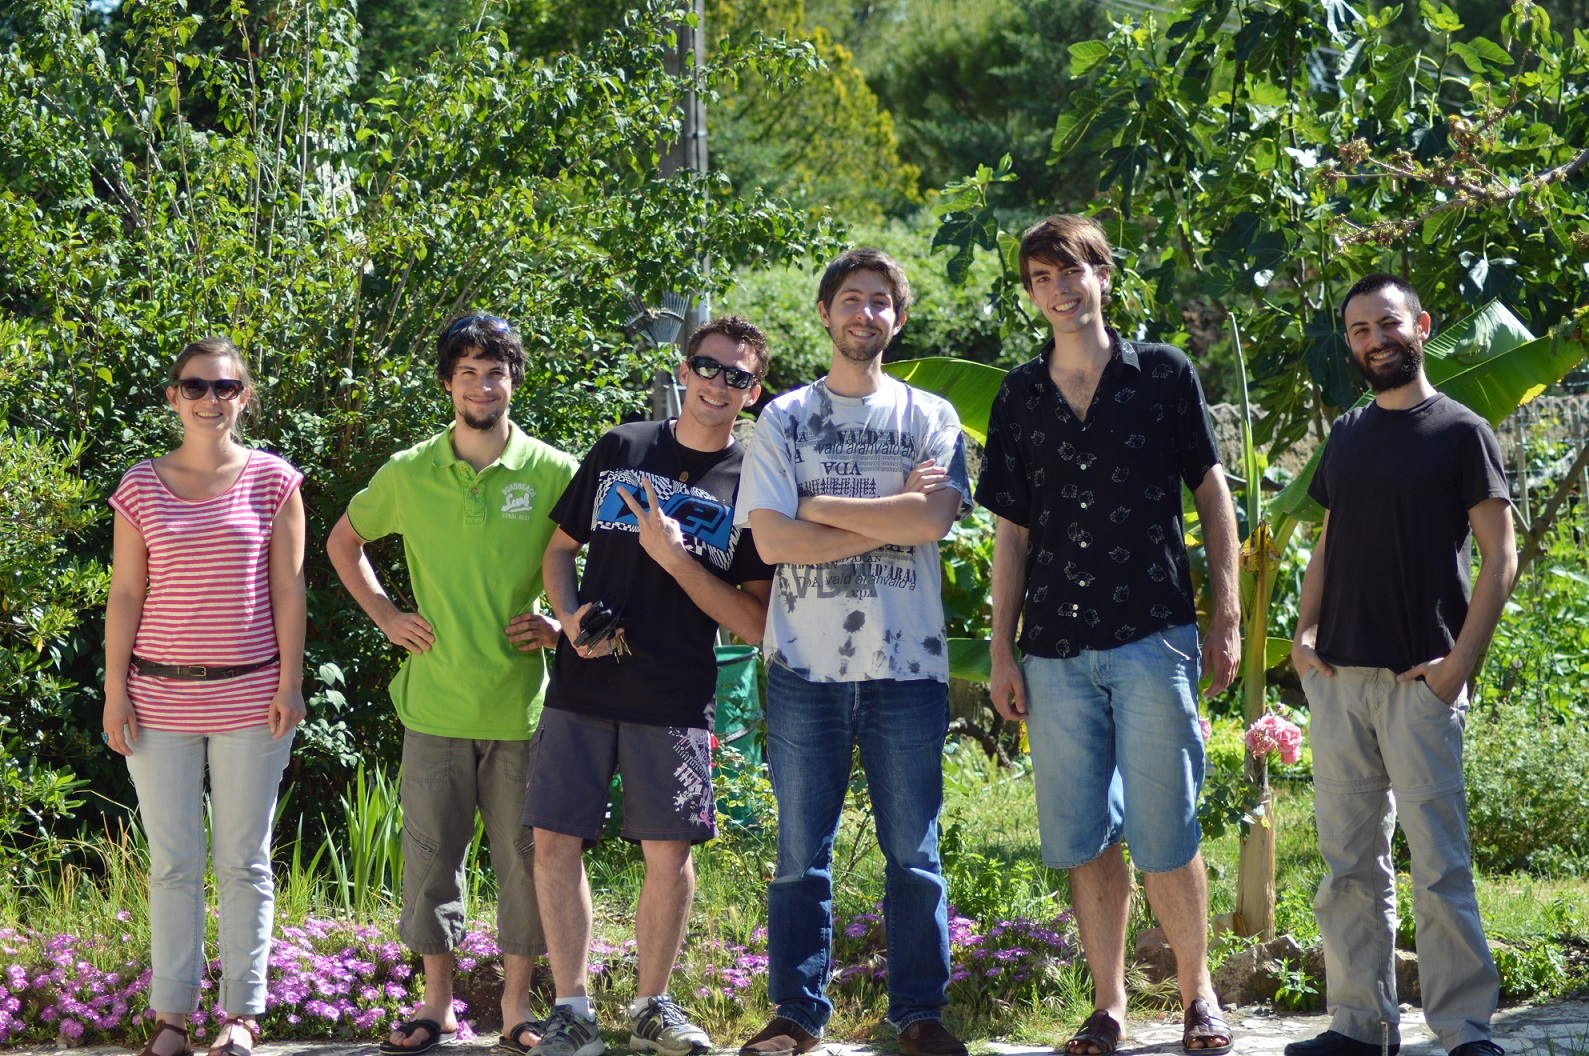
\includegraphics[width=420px]{images/naturalpad_groupe.jpg}
		\caption{Une partie de l'équipe de NaturalPad à Prades le Lez}
		\label{naturalpad_groupe}
	\end{figure}
	
		\subsubsection*{Antoine SEILLES - Fondateur, CEO}
\begin{minipage}[t!]{0.2\linewidth}
\centering

\includegraphics[width=0.8\textwidth]{images/tetocarre/antoine}
\end{minipage}
\begin{minipage}[t!]{0.79\linewidth}
Antoine Seilles est docteur en informatique. Sa thèse, soutenue en avril 2012 porte sur les usages du Web 3.0 (ou web socio-sémantique) dans le contexte de la démocratie électronique. Les domaines de recherche d’Antoine portent essentiellement sur l’aspect social du Web, thème sur lequel il a participé à plusieurs conférences grand public, et sur le Web sémantique, thème sur lequel il a publié à plusieurs reprises et traduit le livre de Tom Heath et Christian Bizer «Linked Data».
		\begin{quotation} \emph{Au sein de NaturalPad} \end{quotation}
Chez NaturalPad, la recherche d’Antoine porte sur les solutions Web 2.0 autour du Dossier Médical Personnel et sur les formats de données utilisant les technologies du Web sémantique (RDF notamment) pour la télémédecine.
\end{minipage}

		\subsubsection*{Sébastien ANDARY - Fondateur}
\begin{minipage}[t!]{0.2\linewidth}
\centering

\includegraphics[width=0.8\textwidth]{images/tetocarre/seb}
\end{minipage}
\begin{minipage}[t!]{0.79\linewidth}
Il a reçu le diplôme de Master d’Informatique à l’Université de Montpellier et termine actuellement un Doctorat de Robotique au LIRMM. Sa thèse porte sur la commande des systèmes mécaniques sous-actionnés dans le cadre de la robotique humanoïde. 
		\begin{quotation} \emph{Au sein de NaturalPad} \end{quotation}
Sébastien travaille au développement de technologies et outils innovants pour la captation de mouvements.
\end{minipage}

		\subsubsection*{Inès DI LORETO - Fondatrice}
\begin{minipage}[t!]{0.2\linewidth}
\centering

\includegraphics[width=0.8\textwidth]{images/tetocarre/ines}
\end{minipage}
\begin{minipage}[t!]{0.79\linewidth}
Elle est diplômée en philosophie et a obtenu un doctorat en informatique à l’Università degli Studi di Milano (Italie). Fin 2009, elle rejoint en postdoc le projet \href{http://www.mojos.fr}{MoJOS}. Dans ce projet de recherche sur les jeux thérapeutiques elle a mené des activités scientifiques pour relever les défis de l’acceptation des patients et des thérapeutes du jeu comme moyen de rééducation. 
		\begin{quotation} \emph{Au sein de NaturalPad} \end{quotation}
Inès travaille sur la transformation des objectifs thérapeutiques en objectifs de jeu en collaboration directe avec les professionnels de la santé.
\end{minipage}

		\subsubsection*{Tristan LE GRANCHE - Fondateur}
\begin{minipage}[t!]{0.2\linewidth}
\centering

\includegraphics[width=0.8\textwidth]{images/tetocarre/tristan}
\end{minipage}
\begin{minipage}[t!]{0.79\linewidth}
Travaillant dans le monde du cinéma d’animation depuis plus de 4 ans, il a travaillé sur plus d’une dizaine de projets de séries télévisées, et de longs et courts métrages. Aujourd’hui il s’est spécialisé dans les Effets Spéciaux Numériques et travaille à l’international en tant que Directeur Technique.
		\begin{quotation} \emph{Au sein de NaturalPad} \end{quotation}
Tristan occupe le poste de Directeur Artistique.
\end{minipage}
	
		\subsubsection*{Benoit LANGE - Fondateur}
\begin{minipage}[t!]{0.2\linewidth}
\centering

\includegraphics[width=0.8\textwidth]{images/tetocarre/ben}
\end{minipage}
\begin{minipage}[t!]{0.79\linewidth}
Il est diplômé d’un master informatique spécialisé en Web et Intelligence Artificielle. Il a ensuite obtenu son diplôme de docteur en informatique à l’université Montpellier 2 en Novembre 2012. Ce doctorat avait pour sujet de réaliser une méthode de visualisation de données afin de permettre l’optimisation énergétique pour le bâtiment. 
		\begin{quotation} \emph{Au sein de NaturalPad} \end{quotation}
Benoit propose, étudie et met en oeuvre des prototypes d’interactions adaptés à des thérapies.
\end{minipage}

		\subsubsection*{Anthony BARREAU - Employé}
\begin{minipage}[t!]{0.2\linewidth}
\centering

\includegraphics[width=0.8\textwidth]{images/tetocarre/anthony}
\end{minipage}
\begin{minipage}[t!]{0.79\linewidth}
Il est diplômé d’une licence professionnelle en informatique spécialité web et gestion. Il a ensuite débuté son expérience professionnelle au sein de l’équipe SMILE du LIRMM. Il a rejoint l’équipe pour participer au développement du projet \href{http://www.mojos.fr}{MoJOS}. Dans ce projet de recherche sur les jeux thérapeutiques, il a participé au développement de prototypes de jeux et d’agents intelligents servant à adapter la difficulté. 
		\begin{quotation} \emph{Au sein de NaturalPad} \end{quotation}
Anthony participe au prototypage et au développement des outils innovants de l’entreprise.
\end{minipage}

		\subsubsection*{Marion FLORIS - Employée}
\begin{minipage}[t!]{0.2\linewidth}
\centering

\includegraphics[width=0.8\textwidth]{images/tetocarre/marion}
\end{minipage}
\begin{minipage}[t!]{0.79\linewidth}
Titulaire d’un D.U.T. Information-Communication et d’une Licence Professionnelle Management des Ressources Numériques, Marion est issue d ’une formation littéraire. Après avoir été libraire spécialisée en bande dessinée pendant deux ans, elle a développé son expertise en Community Management par une formation de 6 mois chez Objectif3D.
		\begin{quotation} \emph{Au sein de NaturalPad} \end{quotation}
Marion est Community Manager et est chargée de la communication.
\end{minipage}

		\subsubsection*{William DYCE - Stagiaire}
\begin{minipage}[t!]{0.2\linewidth}
\centering

\includegraphics[width=0.8\textwidth]{images/tetocarre/william}
\end{minipage}
\begin{minipage}[t!]{0.79\linewidth}
William effectue son stage de Master 2 IMAGINA en même temps que moi chez NaturalPad. L'objectif de son stage était de permettre une reconnaissance des joueurs et de leurs mouvements plus fine avec la Kinect. L'utilisation du Kinect dans un contexte thérapeutique exige en effet une reconnaissance avec des contraintes plus poussées que pour une utilisation purement ludique. Grâce à cela, il sera possible d’imaginer de nouveaux gameplay de jeux basés sur le mouvement.
\end{minipage}

		\subsubsection*{Andy CAMICCI - Stagiaire}
\begin{minipage}[t!]{0.2\linewidth}
\centering

\includegraphics[width=0.8\textwidth]{images/tetocarre/andy}
\end{minipage}
\begin{minipage}[t!]{0.79\linewidth}
Étudiant en licence professionnelle Activité et Techniques de Communication à Arles, Andy a effectué un stage de trois mois de Avril à Juin durant lesquels il a participé au développement de l'interface web thérapeutique et aux modules de visualisation des données de jeux. Nous avons travaillé conjointement afin de fournir un outil ergonomique et efficace pour la paramétrisation des parties des jeux thérapeutiques présents sur la plateforme.
\end{minipage}
		
		\subsubsection*{Kevin BRADSHAW- Stagiaire}
\begin{minipage}[t!]{0.2\linewidth}
\centering

\includegraphics[width=0.8\textwidth]{images/tetocarre/kevin}
\end{minipage}
\begin{minipage}[t!]{0.79\linewidth}
Actuellement en stage, Kevin est en licence Informatique et souhaite devenir developpeur de jeux vidéo. Durant son stage, il concoit et développe son propre jeu de manière indépendante : Zether. Pour cela, il crée les assets graphiques, le son et les diverses fonctionnalités du jeu. \\
Ce jeu a pour dessein de venir se greffer sur la plateforme web de NaturalPad. Kevin a en effet imaginé un gameplay jouable à la fois avec souris+clavier et par les mouvements du corps avec une caméra Kinect. Utilisant une approche différente de la mienne, l'objectif thérapeutique n'est pas clairement défini bien que pris en compte. La plateforme de NaturalPad veut aussi pouvoir accueilir des jeux qui ne sont initialement pas développés dans une optique de rééducation mais dont une telle utilisation est possible.
\end{minipage}
		
		\subsubsection*{Célia GIRONNET - Stagiaire}
\begin{minipage}[t!]{0.2\linewidth}
\centering

\includegraphics[width=0.8\textwidth]{images/tetocarre/celia}
\end{minipage}
\begin{minipage}[t!]{0.79\linewidth}
Stagiaire infographiste, cette étudiante de SupInfoGame contribue à enrichir le monde de Hammer \& Planks en réalisant les modèles 2D et 3D des personnages, monstres et autres décors de cet univers de pirates !
\end{minipage}

	\subsection{Hammer \& Planks}
Hammer \& Planks est le premier jeu sérieux pour la santé de NaturalPad. Il a été conçu en collaboration avec une ergothérapeute, Anaïs Ivorra, dans le but de permettre aux personnes hémiplégiques de retrouver leur faculté d’équilibre. Il a été présenté à diverses occasions lors de salons, qu’ils soient grand public comme le MIG ou spécialisés (\href{http://www.ted.com/tedx/events/5188}{TEDx Montpellier} / \href{http://www.e-virtuoses.net/}{e-virtuoses}). Il a par ailleurs été primé aux e-virtuoses 2013 de Valenciennes dans la catégorie "Serious Game Healthcare" et est largement cité dans un article composé d'une vidéo sur les Serious Game thérapeutiques sur le \href{http://videos.doctissimo.fr/sante/recherche/serious-game-therapeutique.html}{site de doctissimo}.
		
\begin{figure}[htbp]
	\begin{minipage}[c]{.45\linewidth}
		\begin{center}
			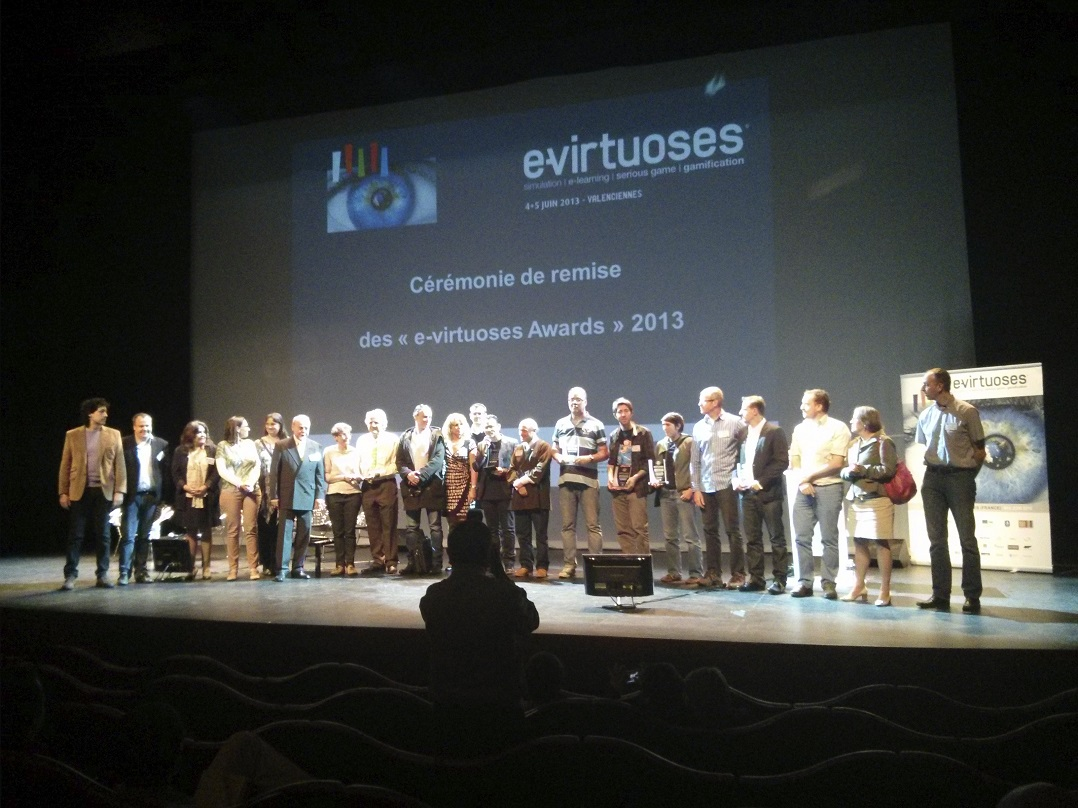
\includegraphics[width=210px, height=157px]{images/remise_awards_e-virtuoses_groupe.jpg}
			\caption{Gagnants des e-virtuoses 2013 dans les différentes catégories.}
			\label{Gagnants}
		\end{center}
	\end{minipage}
	\hfill
	\begin{minipage}[c]{.45\linewidth}
		\begin{center}
			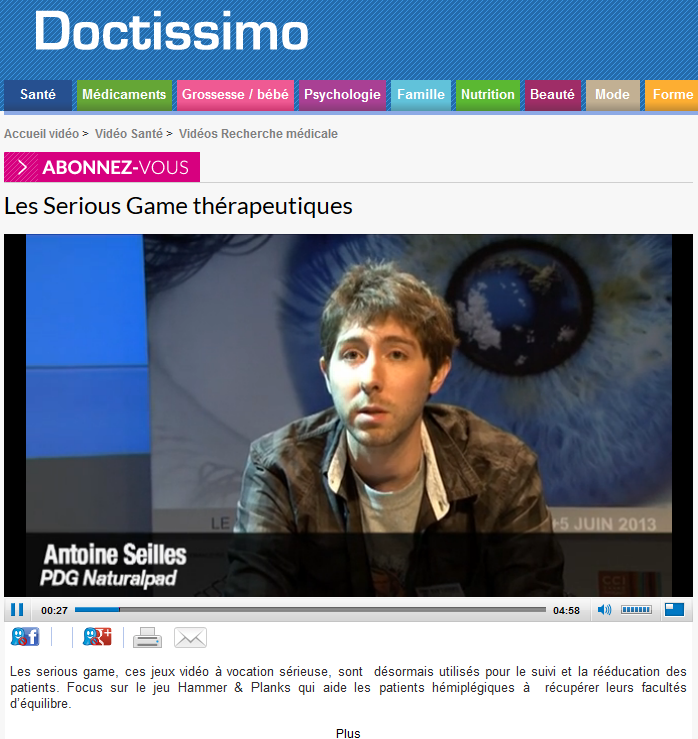
\includegraphics[height=157px]{images/doctissimo.png}
			\caption{Article de doctissimo sur les Serious game thérapeutiques.}
			\label{naturalpad_groupe}
		\end{center}
	\end{minipage}
\end{figure}		

Hammer \& Planks est constitué d’un environnement 3D vu de dessus. Le joueur contrôle un bateau qu'il peut déplacer de gauche à droite et de haut en bas, et peut éliminer les ennemis grâce à ses canons. Enfin, il doit éviter des obstacles et peut récupérer des bonus. Pour contrôler le bateau, il existe plusieurs solutions : on peut utiliser la Kinect, la Wii Board, une manette ou bien le clavier et la souris. Le jeu a initialement été conçu pour une utilisation avec la Wii Board afin de travailler les facultés d'équilibre, que ce soit assis ou debout. Le jeu possède par ailleurs un ensemble de paramètres qui peuvent être paramétrés ou changés en cours de partie, rendant ainsi le jeu devient ajustable selon les besoins thérapeutiques. On notera qu'il existe une version grand public du jeu, où la paramétrisation avancée est remplacée par un enrichissement du gameplay et du scénario notamment.
	\begin{figure}[!t]
		\centering
		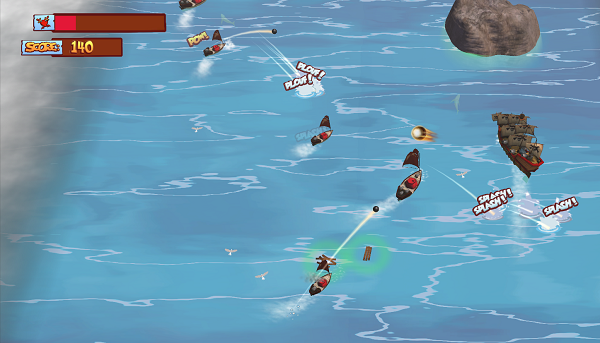
\includegraphics[width=420px]{images/hammer_and_planks.png}
		\caption{Impression d'écran du jeu Hammer \& Planks}
		A droite, le bateau contrôlé par le joueur.
		\label{hammer_and_planks}
	\end{figure}
 
	
	\newpage
	\section{Problématique}
	\subsection{Sujet et objectifs initiaux}
	Dans ce stage, nous allons nous intéresser à l’adaptation de la difficulté dans un jeu à but thérapeutique sous contrôle d’un médecin. Les variables permettant d’ajuster la difficulté d’un jeu sont nombreuses et variées. Elles peuvent être facilement modifiées et combinées pour créer des objectifs de jeu. Cependant, ces objectifs de jeu n’ont pas nécessairement un sens pour le médecin. Il s’agira dans ce stage de définir avec un thérapeute les variables ou paramètres adaptées à l’adaptation de la difficulté pour le soignant.
	\paragraph{}
	Dans le cadre de ce stage, le stagiaire aura pour mission de:
	\begin{itemize}
		\item {récupérer auprès d’un soignant une liste exhaustive d’objectifs de jeu thérapeutique}
		\item {traduire ces objectifs en paramètres dans le jeu Hammer \& Planks}
		\item {proposer une solution pour suivre et analyser visuellement les progrès du patient relativement aux objectifs fixés par le soignant}
	\end{itemize}
	Le stagiaire devra participer à des séances de coconception avec un thérapeute et sera amené à se déplacer pour suivre des séances de tests auprès de patients.
		
\subsection{Contexte et besoins}
Lors de mon arrivée au sein de NaturalPad, il existant déjà une version du jeu Hammer \& Planks, outil dans lequel devait s'insérer mon travail. Présenté lors du MIG 2012, le jeu était encore surtout orienté grand public. Ma première mission fut donc de m'approprier l'application et de l'adapter pour une utilisation paramétrable dans un contexte thérapeutique. En effet, une utilisation thérapeutique implique d'ajuster les différents paramètres en fonction des capacités et des besoins du patient.

	\paragraph{}Les échanges avec les professionnels de la santé ont été au coeur de mon stage. La compréhension des besoins et des contraintes médicales étant primordiales pour proposer un produit adapté, je me suis naturellement tourné vers les thérapeutes et soignants pour acquérir les connaissances et le background qu'il me manquait. Il m'est par ailleurs rapidement apparu qu'on ne pouvait répondre aux différents besoins thérapeutiques explicités par les soignants avec un seul jeu vidéo, même paramétrable. C'est pourquoi je me suis aussi concentré sur l'aspect de conception avec les thérapeutes. 

	\paragraph{Orientation du travail de stage \\}
Rappelons que la société NaturalPad propose comme outil une plateforme web permettant d'accéder à des jeux sérieux, et de les paramétrer directement depuis celle-ci. Hammer \& Planks constitue ainsi le premier jeu accessible depuis cette plateforme et, bien que servant d'exemple des possibilités d'un jeu vidéo pour la santé, il est amené à être rejoint par d'autres serious games. C'est dans cette optique que mon travail durant ce stage s'est progressivement orienté vers une méthode de conception de serious games pour la santé. Cela a pour objectif de proposer une solution appropriée aux différents besoins et contraintes de chaque situation. Ces derniers peuvent correspondre aux objectifs thérapeutiques, à la pathologie du patient, ses capacités, son âge, sa maitrise des nouvelles technologies ou son aisance avec les jeux vidéo par exemple.
Ce travail s'inscrit donc toujours dans le but d'adapter le jeu vidéo aux besoins thérapeutiques, et est complémentaire à une adaptation des paramètres de jeux, qu'elle soit manuelle ou automatique.
 
\paragraph{}Pour cela, je redéfinirais le sujet de ce stage comme suit :\\
\textcolor{marron}{\emph{ {\large Proposition d'une méthodologie de conception de jeux vidéo sérieux à but thérapeutique, et adaptation de la difficulté.}}}

\subsection{Outils et méthodologie}
	\subsubsection{Méthodologie}
Afin de mener à bien ses projets, l’équipe de NaturalPad emploie une méthode Agile de gestion de projet : SCRUM.

	\paragraph{\emph{Méthodes AGILES}\\}
Les méthodes Agiles sont des groupes de pratiques, réunies dans l'\emph{Agile Manifesto}\cite{Agil01}, s'appliquant dans la gestion de projets, généralement informatiques. Ces méthodes se veulent plus pragmatiques que les méthodes traditionnelles et diffèrent de celles-ci en se concentrant sur des valeurs humaines plutôt que sur les processus. Ce sont des méthodes itératives (ou plutôt semi-itératives), incrémentales et adaptatives.
\begin{figure}
	\centering
	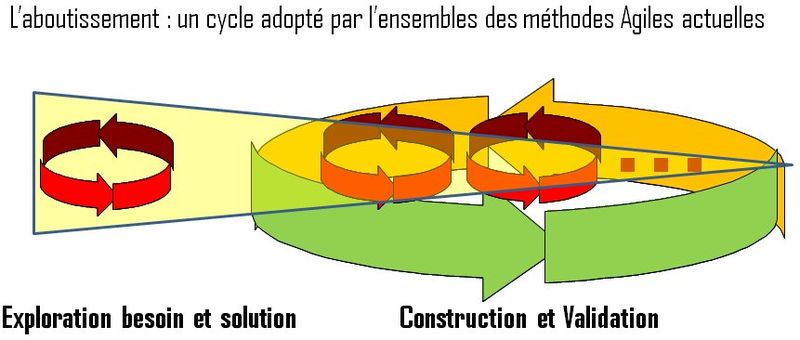
\includegraphics[scale=0.5]{images/agile.jpg}
	\caption{Les méthodes agiles : un cycle semi-itératif}
	\label{agile}
\end{figure}
 
\paragraph{}
Les méthodes agiles prônent 4 valeurs fondamentales :
	\begin{enumerate}
		\item l'équipe : « Les individus et leurs interactions, plus que les processus et les outils. »
		\item L'application : « Des logiciels opérationnels, plus qu'une documentation exhaustive. »
		\item  La collaboration : « La collaboration avec les clients, plus que la négociation contractuelle. »
		\item L'acceptation du changement : « L'adaptation au changement, plus que le suivi d'un plan. »
	\end{enumerate}

		\paragraph{\emph{La méthode Scrum}\\}
Celle-ci définit 3 rôles :
	\begin{itemize}
		\item Le Product Owner
		\item Le Scrum Master
		\item Le Développeur
	\end {itemize}
Le Product Owner est le représentant des clients et des utilisateurs. Son objectif est de maximiser la valeur du produit développé. Il a pour rôle de rédiger des User Stories (comparables à des cas d'utilisation) et de valider le travail des développeurs. 
\\Le ScrumMaster est le responsable de la méthode. Il doit s’assurer qu’elle est correctement mise en application et comprise par les développeurs. Il organise le «Daily Scrum» (voir définition plus bas).
\\Enfin, le Développeur, représente en fait une équipe pluridisciplinaire et auto-organisée : toutes les décisions sont prises ensemble, sans hiérarchie externe ni interne.
 
		\paragraph{Daily Scrum :}
Il s’agit d’une réunion quotidienne ayant pour but de faire un point sur la coordination entre les tâches et les difficultés rencontrées.  Trois questions sont posées aux développeurs : 
	\begin{itemize}
		\item Qu’as-tu fait hier ?
		\item Qu’est-ce que tu vas faire aujourd’hui ?
		\item Est-ce que tu as rencontré des difficultés ?
	\end {itemize}
	
\paragraph{}Le travail est organisé sous forme de sprint. Il s’agit d’une courte période (au maximum un mois) au bout de laquelle l’équipe doit fournir une version améliorée du produit. Chaque sprint possède un but (ex : «on doit pouvoir envoyer des paramètres au jeu») et une liste de tâches (ex : «déterminer la méthode de communication, etc...»). Dès la fin d’un sprint, un nouveau est lancé.

\paragraph{}Enfin, une réunion a lieu en fin de sprint pour faire le point sur le travail accompli, les erreurs rencontrées et comment ne pas les éviter à l'avenir, ainsi que lancer le sprint suivant. Cette méthode est très intéressante car elle permet vraiment de garder une cohésion dans l’équipe de développement et d’avancer de manière visible. 

	\subsubsection{Outils}
		\paragraph{Gestion de projet\\}
Lors de mon arrivée dans l'entreprise, l’équipe utilisait Redmine, une application web de gestion de projets. Nous avons cependant changé deux fois d'outils de gestion de projet pendant la période de ce stage. Le premier est intervenu car les mises à jour des tâches dans Redmine étaient longues et l'outil finalement peu approprié à une méthodologie AGILE, ce qui freinait son utilisation. Nous avons donc mis en place une méthode Kanban qui consiste à écrire chaque tâche sur un post-it, et de déplacer ce post-it dans des colonnes «A faire», «En cours», «Terminé» ou «Validé» selon son avancement par exemple. De cette manière, l’avancement global était bien plus visible mais cette solution était finalement gourmande en post-it et en place. C'est pourquoi, nous utilisons désormais \href{www.trello.com}{Trello}, un outil de gestion de projet en ligne, se basant sur la méthode Kanban. Il s’agit d’un tableau virtuel dans lequel nous pouvons facilement déplacer les tâches, ajouter des commentaires ou des contraintes de temps notamment.

	\begin{figure}[!h]
		\centering
		
\includegraphics[height=48px]{images/redmine.jpg}
		
\includegraphics[height=48px]{images/trello.jpg}
		\caption{Logos de Redmine et Trello}
		\label{logos_redmine_trello}
	\end{figure}
 \newpage
		\paragraph{Développement}
		\subparagraph{} \emph{Unity3D\\}
La majeure partie technique de mon travail a été réalisée pour Hammer \& Planks, qui est développé avec le moteur de jeu Unity3D. Au fil de mon stage, nous sommes passés de la version 3.9 à la version 4.1. Unity permet de facilement intégrer les modèles 3D des objets réalisés dans les logiciels de modélisation 3D tels que Photoshop, Gimp ou Maya. Il propose aussi des options permettant d'utiliser un gestionnaire de versions pour les fichiers du projet.
	\begin{figure}[!h]
		\centering
		
\includegraphics[height=48px]{images/unity.jpg}
		\caption{Logo d'Unity3d}
		\label{logo_unity}
	\end{figure}

		\subparagraph{} \emph{Play! Framework\\}
Play! Framework est un framework open source web qui permet d'écrire rapidement des applications web en Java ou en Scala. Il vise à apporter un outil simple et productif sur la machine virtuelle Java. Play Framework a pour particularité de ne pas être basé sur le moteur Java de Servlet. Il propose par ailleurs un moteur de template basé sur Scala.
	\begin{figure}[!h]
		\centering
		
\includegraphics[height=48px]{images/play.png}
		\caption{Logo de Play! Framework}
		\label{logo_play}
	\end{figure}		

		\subparagraph{} \emph{Git\\}
Que ce soit pour Hammer \& Planks ou nos autres projets en cours, l'utilisation d'un gestionnaire de versions se révèle vite indispensable. Travaillant en équipe allant jusqu'à cinq développeurs et une graphiste, il est nécessaire de pouvoir mutualiser le travail. De plus, l'expérimentation et le développement de nouveaux éléments se prêtent très bien à l'utilisation de plusieurs branches de développement, chose que Git permet de gérer facilement.
	\begin{figure}[!h]
		\centering
		
\includegraphics[height=48px]{images/git.png}
		\caption{Logo de Git}
		\label{logo_git}
	\end{figure}

		\subparagraph{}	\emph{BitBucket et GitHub}
Pour héberger ses projets, NaturalPad avait l'habitude d'utiliser GitHub. Avec l'arrivée de nouveaux stagiaires, il nous a fallu trouver une solution permettant un accès privé au dépôt pour un plus grand nombre de personnes, ce que permet BitBucket.
	\begin{figure}[!h]
		\centering
		
\includegraphics[height=48px]{images/bitbucket.jpg}
		
\includegraphics[height=48px]{images/github.jpg}
		\caption{Logos de BitBucket et Github}
		\label{logos_bitbucket_github}
	\end{figure}

	\subsubsection{Veille}
Le Jeu Vidéo et plus généralement l'Informatique est un domaine en constante évolution dans lequel il est nécessaire de se tenir à jour pour connaître les dernières technologies et actualités. Pour cela, j'ai observé durant l'intégralité de ma période de stage une veille technologique et stratégique. Nouveautés technologiques, logiques ou matérielles, communications d'entreprises ou de salons nationaux et internationaux ou bien encore annonces de sociétés dont le secteur d'activité est compatible avec NaturalPad ont donc été au coeur de mon étude quotidienne.
\paragraph{}Pour faciliter ce travail de veille, par ailleurs inclu dans mon planning, j'utilise un agrégateur de flux RSS, outil indispensable pour gérer aisément un contenu important sur un grand nombre de sources différentes. Il s'agit ensuite de mettre à jour et d'étendre régulièrement les sources en fonction de l'utilité observée de chacune d'entre elle ou des manques ressentis. 
\paragraph{Jeux Vidéo\\ \quad}
Étant étudiant en Informatique, option Image Game and Intelligent Agents, et ayant orienté ma formation vers une spécialité Jeux Vidéo, il m'a semblé important de me tenir à jour en terme d'actualité vidéoludique. J'ai pour cela étendu ma veille aux domaines des jeux vidéo, indépendants ou blockbusters, afin d'en étudier différents aspects tels le business model, le gameplay, les technologies employées ou les mécanismes de jeu innovants par exemple. J'ai ainsi pu testé des technologies récentes comme la console Ouya ou le système de contrôle Leap Motion, qui permet d'interagir en utilisant ses mains et ses doigts. Pour plus d'informations sur le Leap Motion, vous pouvez retrouver mon billet sur le blog de \href{naturalpad.fr/category/naturalblog}{NaturalPad}.
\begin{figure}
	\centering
	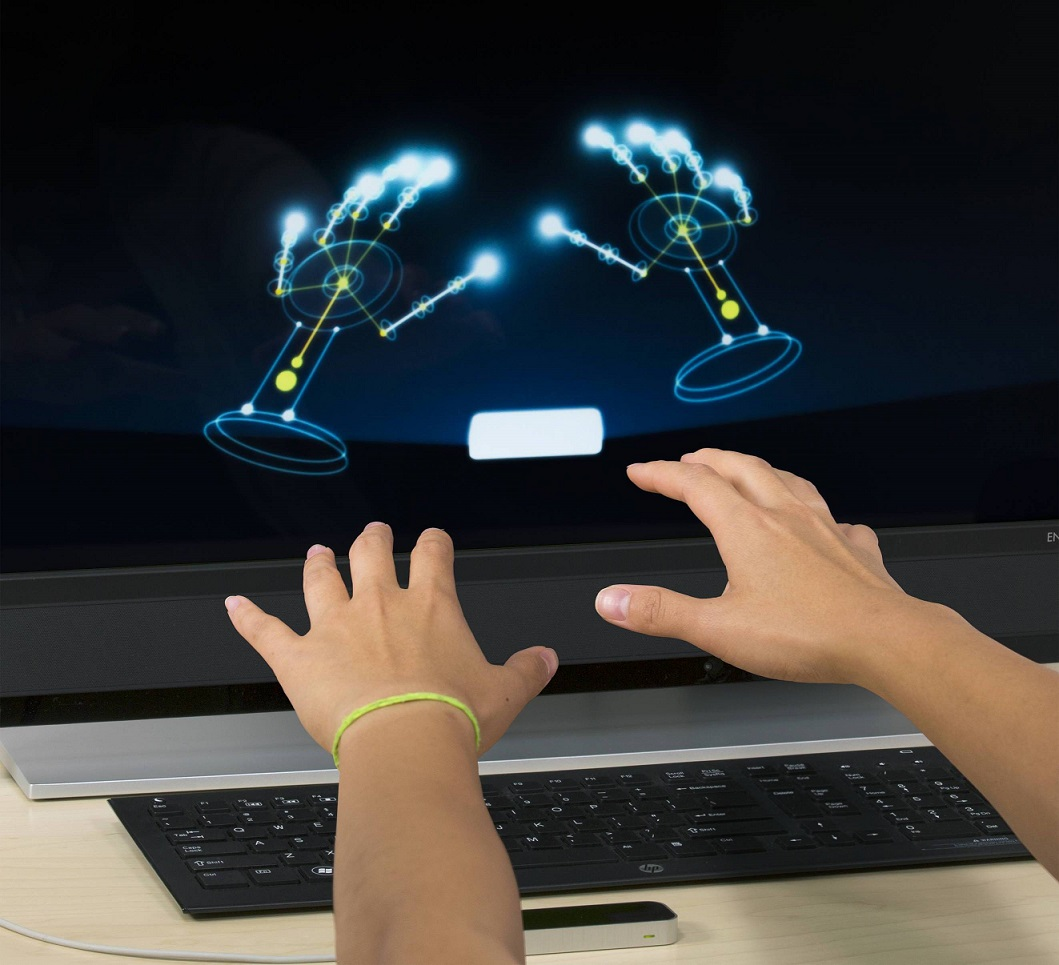
\includegraphics{images/leap_motion.jpg}
	\caption{Utilisation d'un Leap Motion}Une application retranscrit à l'écran la "vision" qu'elle a des mains de l'utilisateur.
	\label{leapmotion}
\end{figure}

	\subsubsection{État de l'art et recherche documentaire}
Étendue sur plusieurs semaines, la réalisation de l'état de l'art était pour moi quelque chose de nouveau qui a nécessité une certaine organisation. Deux moments ont été importants : la phase de démarrage et l'arrêt des recherches. Commencer ces recherches alors que les sujets que je devais ou voulais couvrir étaient vastes et non clairement définis fut à la fois plaisant et compliqué. Bien que beaucoup de choses me semblaient intéressantes, la question était de savoir par où commencer. De la même manière, au fil de mes lectures, je découvrais de nouveaux liens et références présentant de nouveaux aspects qui eux-même renvoyaient vers d'autres solutions et articles. La difficulté était donc de juger quand mes connaissances sur un thème donné étaient suffisantes pour éviter de poursuivre d'interminables recherches, aussi intéressantes puissent elles être, le temps étant limité dans le cadre d'un stage de Master.
	\paragraph{}Au niveau des lectures abordées, ma source principale fut des articles scientifiques, suivie par des articles de magazines spécialisés et articles web notamment. Pour les thèmes médicaux, un certain nombre d'articles m'a été directement conseillé par des professionnels de la santé, articles à partir desquels j'ai ensuite pu compléter mon état de l'art en suivant les références. Par ailleurs, il est fréquent que certains auteurs ressortent régulièrement lorsqu'on effectue des recherches sur un thème donné, ce qui permet, en plus du nombre de citations des articles, de rapidement cerner quels sont les articles et chercheurs de référence dans le domaine.
	\paragraph{}Bien entendu, afin de rendre mes lectures efficaces, je me constituais pour chacune d'elle une fiche de lecture où noter les points importants : 
\begin{itemize}
	\item Titre ou source
	\item Auteur(s)
	\item Mots clefs
	\item Synthèse
	\item Jugement personnel ou remarques
	\item Références importantes
\end{itemize}
	
	\newpage
	\section{Background}
	\subsection{Jeux vidéo}
	%%Définition d'un Jeu 
	\subsubsection*{Définition d'un Jeu}
Le jeu vidéo est un média participatif en pleine extension et de plus en plus largement accepté et plébiscité par la population. \\Dans sa définition, un jeu vidéo est une extension du jeu au monde numérique en utilisant les technologies informatiques. Il s'agit donc en amont de bien comprendre ce qu'est un jeu. \\Dans son travail d’analyse, Juul\cite{Juul05} donne une synthèse qui regroupe les points partagés par toutes les définitions existantes~:
\begin{quotation}
A game is a rule-based formal system with a variable and quantifiable outcome, where different outcomes are assigned different values, the player exerts effort in order to influence the outcome, the player feels attached to the outcome, and the consequences of the activity are optional and negotiable. 
\end{quotation}
\paragraph{Points clefs \\}
Les 6 points clefs identifiés par Juul sont :
\begin{itemize}
	\item les règles
	\item le résultat quantifiable variable
	\item la valorisation du résultat
	\item l’effort du joueur
	\item l’attachement du joueur au résultat (identifié par Gendler comme Alief, 2009)
	\item des conséquences négociables.
\end{itemize}

		\subsubsection*{Pratique et consommation des jeux vidéo}
Le jeu vidéo est un média récent qui trouve ses origines dans le début de la seconde moitié du XX$^{eme}$ siècle. D'abord majoritairement accessibles sur des bornes d'arcade, les jeux vidéo se sont progressivement répandus avec la commercialisation de consoles de salon. Selon une étude commandée par le Centre National du Cinéma et de l'image animée\href{http://www.cnc.fr}{(CNC)}, c'est près de 60\% de la population française qui jouaient à des jeux vidéo au cours de l'année 2011\cite{Cnc11}. L'âge moyen des joueurs était alors de 34,7 ans et cette population constituée de 54,1\% d'hommes fin 2011\cite{Cnc11}. L'arrivée de la console Wii et de jeux orientés plus casuals\footnote{Se dit d'une personne ne jouant à des jeux vidéo que de manière occasionnelle. Peut aussi se dire d'un jeu dont la cible sont des joueurs occasionnels.} a permi en France une meilleure diffusion du média au sein de la population, qui accepte de plus en plus de se livrer à cette activité. Contrairement à ce que l'on pourrait croire, notamment à cause de leur méconnaissance des nouvelles technologies et du jeu vidéo plus spécifiquement, les seniors se prêtent aussi volontier à la pratique de ce loisir numérique. C'est une constation que nous avons pu vérifier par nous-même lors de nos différentes sessions de tests au centre hospitalier de Lapeyronie et dans une maison de retraite à Lille, mais aussi dans différentes lectures qui seront détaillées ci-après.
	
		\subsubsection*{Propriétés des jeux vidéo}
En 1984, [Driskell and Dwyer]\cite{Dris84}réalisent un premier état de l'art et trouvent que plusieurs caractéristiques des jeux vidéo peuvent influer sur les propriétés d'apprentissage et de motivation : des objectifs spécifiques, un challenge, de la fantaisie et du mystère. Ils théorisent qu'une augmentation de la motivation produit une augmentation de l'attention et mène à une meilleure mémorisation des acquis (connaissance déclarative) et une focalisation de l'attention (stratégie cognitive).\newline
[Malone et Lepper, 1987] mentionnent le challenge, la curiosité, le contrôle et la fantaisie comme caractéristiques intégrantes des jeux vidéo. Selon [de Felix et Johnson , 1993], les jeux sont composés d'éléments visuels dynamiques, d'interactions, de règles et d'objectifs. Puis [Thiagarajan, 1999] affirme que le conflit, le contrôle, la terminalité et l'artifice sont les quatre éléments nécessaires d'un jeu. En 2001, [Garis and Ahlers, 01] donnent 39 descripteurs qui seront réduits à 12 pour ne garder que les paramètres statistiquement les plus significatifs pour renforcer la sensation de "game-like". \\ Finalement en 2002, [Garris et al] proposent un sous-ensemble de tous ces attributs qui seront considérés commes les paramètres de jeu clefs de l'apprentissage~:
\begin{itemize}
	\item la fantaisie
	\item les règles
	\item la stimulation sensorielle
	\item le challenge
	\item le mystère
	\item le contrôle
\end{itemize}

\paragraph{}En 2009, [Wilson et al]\cite{Wils09} partent de l'ensemble de paramètres de [Garris et al] pour enrichir le modèle avec de nouveaux paramètres qui leur semblent avoir un impact sur l'apprentissage.
Les tableaux \ref{game_attributes_one} et \ref{game_attributes_two} indiquent et décrivent ces douze attributs.

\begin{figure}[htbp]
	\centering
	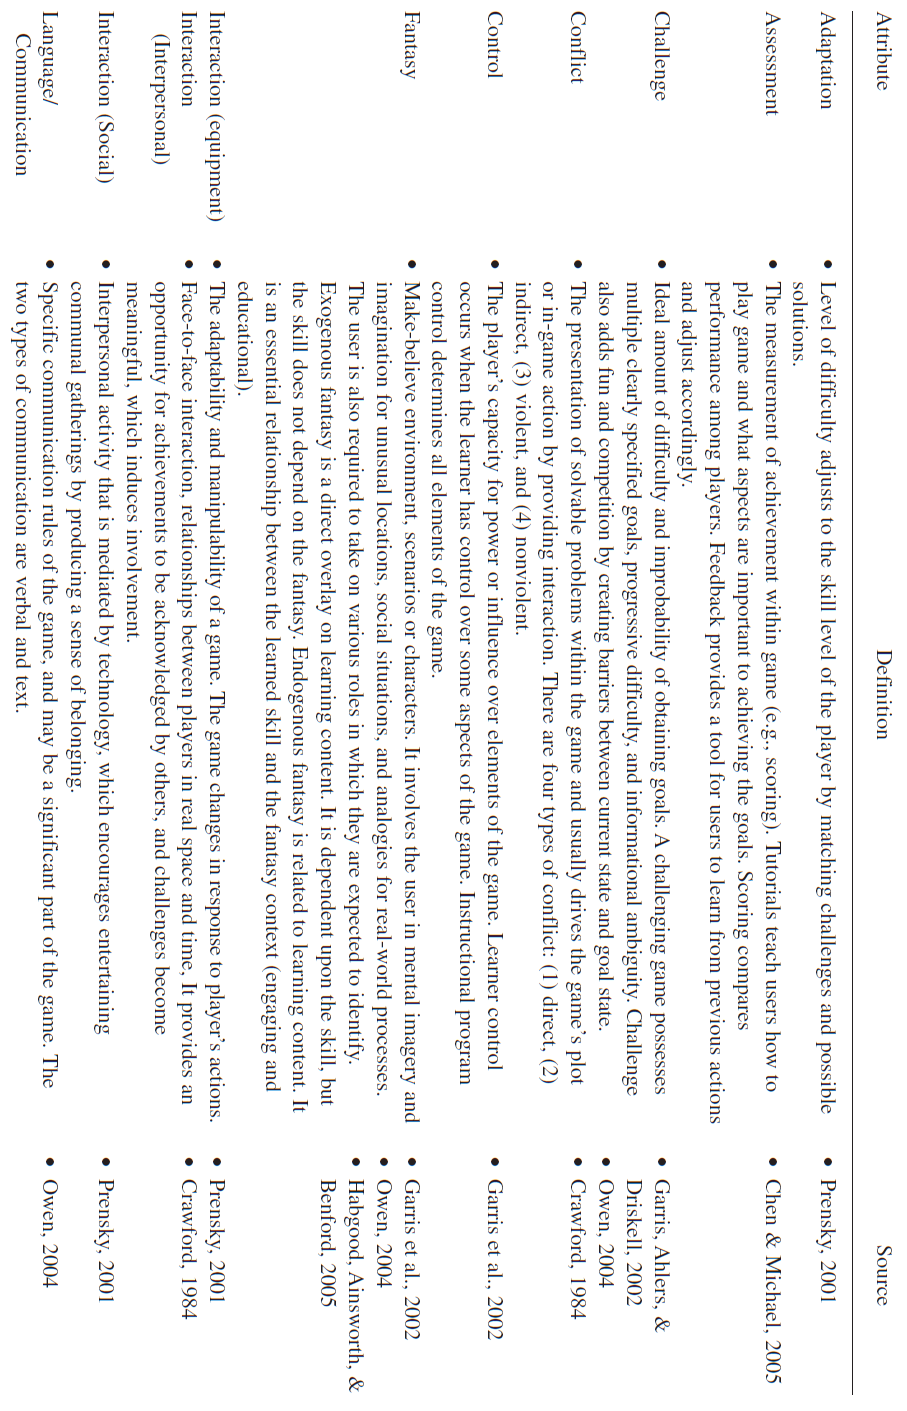
\includegraphics[width=\linewidth, height=\textheight ]{images/game_attributes_one}
	\caption{Propriétés des jeux vidéo et leur définition. (1/2) \cite{Wils09}}
	\label{game_attributes_one}
\end{figure}
\begin{figure}[htbp]
	\centering
	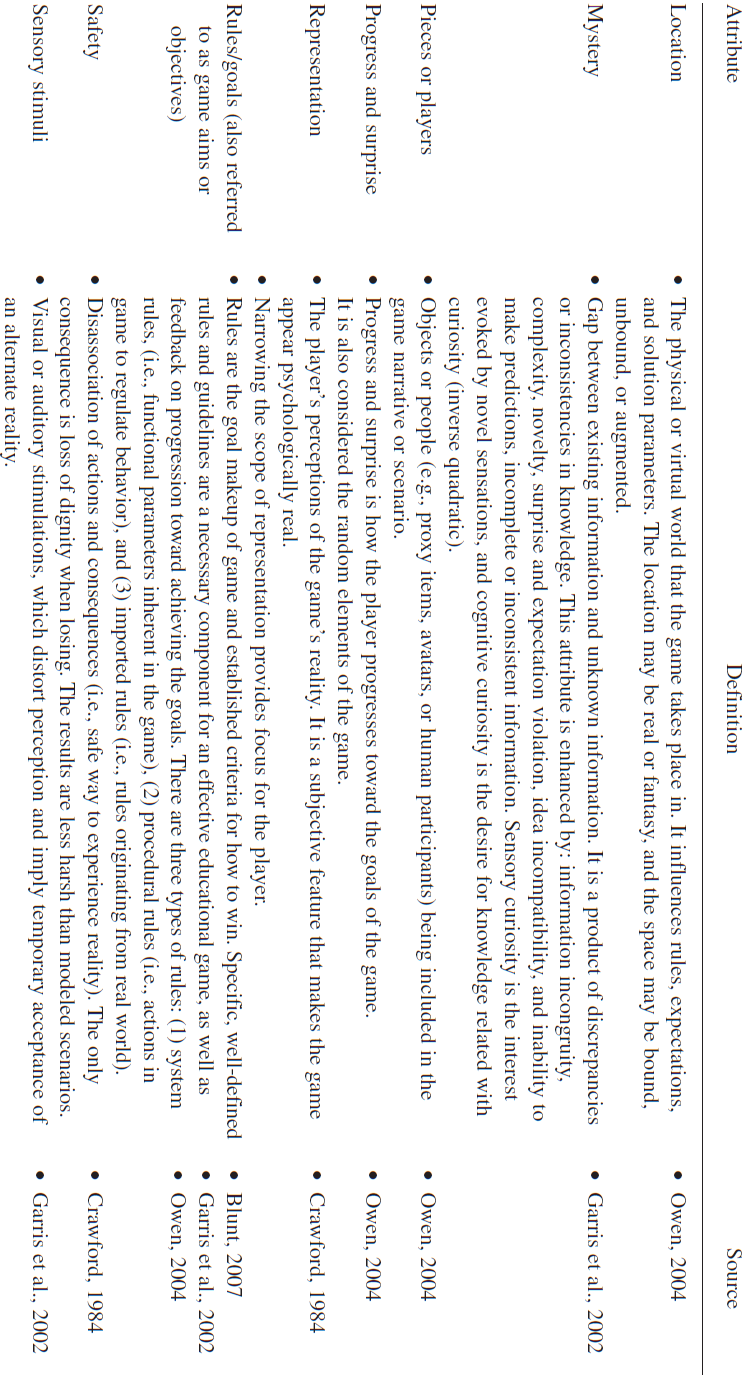
\includegraphics[width=\linewidth, height=\textheight ]{images/game_attributes_two}
	\caption{Propriétés des jeux vidéo et leur définition. (2/2) \cite{Wils09}}
	\label{game_attributes_two}
\end{figure}	
	
	\subsection{Jeux sérieux et Théories Comportementales}
Les jeux vidéo se révèlent être un outil dont l’impact peut dépasser la simple portée ludique. Les serious games se proposent de profiter du ressort ludique du jeu vidéo pour servir volontairement un objectif sérieux distinct. Jeux éducationnels, commerciaux, idéologiques ou d’entraînement font partie de cette famille des jeux sérieux. D’un point de vue thérapeutique, il est possible de les utiliser afin de rendre le travail de réhabilitation ou de remise en forme plus motivant pour le patient en combinant les aspects ludique et thérapeutique.

\paragraph{}
Les jeux vidéo sérieux se présentent comme un potentiel médiateur dans la modification des habitudes comportementales en permettant d’inclure des connaissances pratiques dans un modèle ludique apprécié. Il est possible d’y mettre en place des procédures de changement comme l’établissement d’objectifs ou la modélisation et le développement de compétences dans un environnement attrayant, significatif et immersif [Baranowski et al, 2008]\cite{Bara08}. \\
Les jeux vidéo promeuvent les interactions sociales et d’apprentissage [Wideman et all, 2008], créent un environnement où les actions du joueur ont un effet [Gee, 2004]\cite{Gee04} , encouragent la résolution de problèmes [Gee, 2004]\cite{Gee04} et renforcent la compréhension en créant des situations de réflexion ou en aidant le joueur dans ses objectifs [Gee, 2004]\cite{Gee04}. Enfin, les jeux sérieux pour la santé sont fait pour distraire le joueur tout en l’éduquant, en l’entrainant ou en changeant ses comportements [Stokes, 2005]\cite{Stok05}.

		\subsubsection*{Théories comportementales}
Le comportement est la résultante d’influences multiples, rendant ainsi souvent les personnes réfractaires au changement [Baranowski, Lin \& al, 1997]\cite{Bara97}. Le comportement doit alors être considéré comme un mécanisme complexe découlant de l’enchaînement de plusieurs étapes. Ainsi, plutôt que de chercher à impacter directement le comportement, les experts comportementaux valorisent une action sur ces facteurs intermédiaires, appelés médiateurs. Changer ces médiateurs permet de changer le comportement [Baranowski, Lin \& al 1997]\cite{Bara97}.
\paragraph{}Plusieurs grandes théories comportementales existent~:
\begin{itemize}
	\item la théorie d’inoculation comportementale [McGuire, 1961]
	\item la théorie socio-cognitive [Bandura, 1986]
	\item la théorie de l’auto-détermination [Ryan \& Deci, 2000]
	\item la théorie de l’immersion [Green \& Brock, 2000]
\end{itemize}

\paragraph{}De ces théories, l’on peut alors identifier un certains nombre de ces facteurs médiateurs tels que : l’immersion, l’attention, l’auto-régulation, le développement de compétences, la motivation interne et externe, l’autonomie ou encore le sentiment de compétence. La science du comportement fournit aussi des techniques qui facilitent le changement comportemental, et propose d’utiliser ces facteurs dans les média de divertissement tel que le jeu vidéo.\\
Le modèle : "Elaboration Likelihood Model" [Petty \& Cacioppo, 1986] soutient ainsi que des personnages crédibles, attrayants et sympathiques sont plus susceptibles d’être persuasifs que les autres et peuvent donc servir d’intermédiaires pour véhiculer un message. \\
La théorie d’inoculation comportementale [McGuire, 1961] met en garde contre une possible contre-productivité en identifiant et en réfutant les menaces potentielles à l’accomplissement des objectifs du changement désiré.\\
La théorie socio-cognitive [Bandura, 1986] préconise l’établissement d’objectifs et le développement de compétences comme paramètres importants dans le changement comportemental.\\
Enfin, les théories socio-cognitive [Bandura, 1986] et d’auto-détermination [Ryan \& Deci, 2000] mettent toutes deux l’accent sur l’importance du feedback pour guider et mettre en forme le comportement durant le processus de changement.	

	\subsection{Jeux sérieux thérapeutiques}
Dans notre contexte, l’aspect sérieux recherché du jeu est la réhabilitation motrice ou la rééducation physique du joueur. Ces objectifs sont indiqués par des thérapeutes, médecins ou kinés, notamment dans le cadre de réhabilitation de personnes hémiplégiques ou souffrant de douleurs lombaires. L’intérêt du jeu vidéo est alors de proposer un environnement de réhabilitation plus agréable et de faciliter l’acceptation des travaux de rééducation par le patient grâce aux éléments de gameplay. Le jeu peut permettre un plus grand volume de travail de la part du patient car celui-ci sera plus enclin à les réaliser dans le cadre du jeu sérieux. Surtout, le jeu sérieux augmente la répétition de mouvements, ce qui améliore l'état physique du joueur-patient. L’objectif à terme est donc d’améliorer les résultats de l’objectif thérapeutique.

	\subsubsection*{Contexte socio-médical}
		\paragraph{L'AVC et Hammer \& Planks\\}
Dans les pays occidentaux, près d'un individu sur 600 est victime d'un AVC chaque année, soit près de 120 000 accidents par an en France. L'AVC est une cause fréquente d'hémiplégie chez les victimes et reste une des principales causes d'invalidité. \\
La récupération des fonctions motrices, de la parole ou de la compréhension dépendent pour beaucoup de l'âge du patient et de son atteinte au niveau du cerveau.
\paragraph{}Hammer \& Planks est né d'un projet d'une étudiante en ergothérapie dont le but était de proposer un jeu servant à travailler l'équilibre chez des personnes hémiplégiques ayant été victimes d'un AVC. Aujourd'hui, H\&P peut être utilisé aussi bien pour travailler son équilibre, ses membres supérieurs son tronc ou sa capacité d'attention.

	\subsubsection*{Récupération de lombalgie}
Si la réhabilitation post AVC a été au cœur de mon travail et de celui de NaturalPad, son objectif est de pouvoir proposer ou accéder à des solutions pour divers types de pathologies. Ainsi, un projet de NaturalPad pour lequel j'ai participé à la phase de conception a pour objectif de créer un serious game pour la rééducation de personnes lombalgiques.
\paragraph{}
La lombalgie est un état douloureux du rachis lombaire qui peut être aiguë ou chronique. Les lombalgies affectent une forte proportion de personnes puisque entre 40 et 70\% de la population est touchée à un moment ou un autre. Sous l'effet de la douleur, une majorité des patients va cesser toute activité physique voir même professionnelle. Une de ses conséquences est aussi une démotivation de la personne pouvant aller jusqu'à un état de dépression, notamment dû à l'inactivité et la douleur. Comme préconisé dans le Guide du Dos\cite{backbook}, la reprise et le maintien d'une activité physique sont primordiaux dans le processus de récupération. \\
Le projet de NaturalPad est une application de coaching sportif adaptée à ce besoin et proposant un certain nombre d'exercices physiques gamifiés afin d'encourager la reprise d'activité des utilisateurs.

	\subsection{Réhabilitation}
Un autre aspect est la dimension médicale de la rééducation. Connaître les enjeux, les contraintes, le contexte médico-social d'une réhabilitation ainsi que les techniques existantes s'avérait donc nécessaire. Cette partie est la synthèse de mes entretiens et investigations dans ce domaine qui ne m'était encore que peu connu.

	\subsubsection*{Connaître l'AVC TODO}
Dans les pays occidentaux, l’accident vasculaire cérébral est une cause majeure de handicap acquis de l’adulte, la deuxième cause de démence après la maladie d’Alzheimer et la troisième cause de mortalité.

		\paragraph{\emph{L’accident vasculaire cérébral (AVC) est un événement de santé fréquent}\\}
    En 2008, en France, il y a eu un peu plus de 130 000 hospitalisations pour accident neuro-vasculaire soit « 1 AVC toutes les 4 minutes » se répartissant ainsi :
    - 105 000 hospitalisations pour AVC
    - 31 000 hospitalisations pour accident ischémique transitoire (AIT).

    L’âge moyen de survenue d’un AVC est de 73 ans (70 ans pour les hommes et 76 ans pour les femmes),

    Le nombre de personnes hospitalisées pour AVC a augmenté de 10,9\% entre 2002 et 2008 mais ceci est essentiellement lié à l’augmentation et au vieillissement de la population. En effet le taux standardisé sur l’âge a globalement diminué de 2.6\% sur cette période.

    Cette tendance globale à la baisse s’accompagne pour la première fois d’une augmentation du taux avant 65 ans (+ 10.8\%) combinée à une réduction pour les 65 ans et plus (-6.6\%).

    Les données préoccupantes concernant l’augmentation des AVC dans la population des moins de 65 ans concernent plus les femmes (+ 12,9\%) que les hommes (+9,7\%). Ce phénomène épidémiologique préoccupant est à examiner dans un contexte de diminution de l’espérance de vie en bonne santé ( sans incapacité) qui est passée de 62,7 ans à 61,9 ans pour les hommes et de 64,6 ans à 63,5 ans pour les femmes, en seulement deux ans (entre 2008 et 2010)

L’accident vasculaire cérébral (AVC) est un événement de santé grave :

- En termes de mortalité :

    L’AVC représente la troisième cause de mortalité pour les hommes (après les cancers « de la plèvre, de la trachée, du larynx ou des poumons » et les cardiopathies ischémiques) et la première pour les femmes avant le cancer du sein.

    En 2008, l’AVC a été responsable de 33 000 décès.

    Depuis le milieu des années 70, on observe une baisse continue de la mortalité cérébro-vasculaire (- 50\% entre 1990 et 2008).

- En termes de handicap :

    L’AVC est souvent responsable de séquelles qui affectent la qualité de vie des patients. 

    Les atteintes peuvent être motrices, sensitives, sensorielles et cognitives (avec notamment des troubles de la mémoire) 

    Un mois après l’AVC, pour les personnes ayant survécues, les dépressions sont fréquentes et il est à noter que seulement 41\% d’entre elles n’ont plus de symptômes, ainsi :
    -25\% présentent un handicap léger ou modéré
    -34\% ne peuvent marcher sans assistance.

    L’estimation du nombre de personnes vivant avec des séquelles d’AVC responsables de handicap ne peut se mesurer uniquement à partir des 306 000 personnes enregistrées en affection de longue durée (ALD) pour « AVC invalidant » dans les principaux régimes d’assurance maladie fin 2008.

    Les enquêtes Handicap-Santé auprès des ménages (HSM) et en institution (HSI) ont permis d’estimer à 1,2\% la proportion de personnes ayant déclaré des antécédents d’AVC et à 0,8\% la prévalence des séquelles d’AVC. Ceci correspond à :
    - 771 000 personnes avec antécédent d’AVC sur le territoire national, dont 505 000 présentant des séquelles.
    - Selon les déclarations des patients, les séquelles les plus fréquentes étaient des troubles de l’équilibre et des troubles de la mémoire, puis les paralysies ou parésie d’un ou plusieurs membres et les troubles du langage.
    	
\paragraph{}
Lors de mes six mois de stage, j'ai ainsi été en relation avec plusieurs docteurs en médecine, des kinésithérapeutes ainsi que des ergothérapeutes.

	\subsubsection*{Enjeux et objectifs thérapeutiques de la réhabilitation}\label{objectifs_therapeutiques}
Le principe de base est de faire un bilan initial.  A partir de ce dernier on dégage des objectifs  de rééducation. Pour atteindre ces objectifs, il existe des moyens de rééducation (exercices, physiothérapie, jeux vidéos, etc.) qu'il faut adapter au patient.

\paragraph{Les grand axes de rééducation}
\begin{itemize} 
	\item Récupérer la commande motrice 
	\item Diminuer la douleur
	\item Assouplir les muscles 
	\item Récupérer la sensibilité 
	\item Renforcement musculaire 
	\item Transfert du poids du corps 
	\item Travail de l'équilibre bipodal / unipodal 
	\item Travail du schéma de marche
\end{itemize}

	\textbf{\emph{Définitions}\\}
• \emph{La spasticité} consiste en un étirement rapide d'un muscle qui entraîne trop facilement sa contraction réflexe qui dure un certain temps. \\
• \emph{L’hypertonie spastique} (musculaire) est une contraction réflexe du muscle qui s'oppose à l'étirement.\\

	\textbf{\emph{Signifiant VS significatif}\\}
L’aspect signifiant/significatif est un terme utilisé en ergothérapie pour définir le sens qu'a une activité auprès d’un patient.\\
• Une activité peut être qualifiée de \emph{\textcolor{orange}{significative}} quand elle revêt un \textcolor{orange}{sens social commun}. Par exemple dans notre cadre, les jeux vidéo et notamment la Wii, peuvent être significatifs pour les personne âgées de 10 à 30 ans, car ils sont beaucoup utilisés dans cette tranche d'âge.\\
• Une activité est dite \emph{\textcolor{vert}{signifiante}} quand elle a du sens pour la personne de \textcolor{vert}{manière personnelle}. Par exemple, faire la vaisselle est \textcolor{orange}{significatif }car on \textcolor{orange}{doit} la faire. Mais en général les personnes n’aiment pas la faire et elle est donc pour eux non signifiante. Alors que ‘moi’, c'est une activité que ‘j’’apprécie :  elle a donc pour ‘moi’ un sens motivationnel et est alors signifiante.

	\paragraph{\emph{Cas de l’hémiplégie} \\}
C’est une pathologie qui n’est pas évolutive, on ne peut que récupérer. Cette récupération est différente chez tous les patients, en fonction de leur âge, leur condition physique, de la gravité de la pathologie et de la rééducation mise en place.

	\subsubsection*{Cas de l'hémiplégie : objectifs thérapeutiques}
\paragraph{\emph{Mouvements analytiques / Motricité fine} \\ }
Les hémiplégiques vont présenter des troubles de la sensibilité et des troubles de la commande volontaire. Un problème nerveux peut entraîner une augmentation du tonus musculaire pouvant provoquer une spasticité ou une hypertonie. 

\paragraph{}
Parmi les objectifs, on va donc tout d’abord chercher à récupérer une commande motrice normale, puis à rééquilibrer les capacités (musculaires et nerveuses) et enfin renforcer les capacités musculaires. Dans la pratique, le patient va donc tout d’abord chercher à retrouver un mouvement précis, puis à être capable de l’effectuer de manière fluide et plus rapide, puis à pouvoir mettre de la force dans son geste, pour vaincre la gravité ou supporter un poids/une résistance par exemple.

\paragraph{}
Pour ‘vaincre’ la spasticité du patient, le praticien doit pratiquer des manipulations sur le patient pour étirer ses muscles. Il est donc difficilement envisageable de gamifier cet aspect de la rééducation.\newline
Déficit léger : travail en 3D possible     \quad$ \rightarrow $\quad       Épaules\\
Déficit lourd : travail en 2D uniquement  \quad $\rightarrow $\quad      Poignets et mains

	\paragraph{Paramètres\\}
Récupération de la commande volontaire, amplitude articulaire, spasticité, phase aiguë VS phase chronique( $ \rightarrow $ spastique)\\
Plasticité cérébrale : intensive et ciblée. \newline

Les thérapeutes veulent~: 
\begin{itemize}
	\item des mouvements répétitifs fins
	\item un type précis de mouvement (rotation par exemple)
	\item pouvoir paramétrer les exercices
	\item lâcher / écarter (voir le système PABLO)
\end{itemize}

	\paragraph{\emph{Sensibilité} \\ \quad}
Exercice : le patient ferme les yeux, le thérapeute lui donne un petit objet dans la main. Que ressent-il? Quelle texture, quelle forme? \\
En fait, on lui présente avant l’exercice une série d’objets (éponges de différentes tailles et souplesses, figurines en bois de différentes formes). Puis, yeux fermés, il doit essayer de reconnaître l’objet que lui présente le thérapeute en identifiant ses propriétés haptico-tactiles.
\paragraph{} 
Ce travail de la sensibilité est particulièrement important pour les mains, riches en capteurs tactiles. Il est par ailleurs nécessaires de travailler cet aspect pour que le cerveau “n’oublie pas” en réutilisant les connexions neuronales spécifiques. Par ailleurs, on peut aussi travailler la sensibilité d’autres membres comme les pieds, ce qui est particulièrement important notamment dans le cadre de la marche où la perception des aspérités/irrégularités du sol est importante.\\
Cet aspect de la rééducation est complémentaire de celui de la récupération de la préhension. Le patient aura ainsi la capacité (commande, force) de tenir un objet, mais le lâchera faute d’informations sensorielles suffisantes.

	\paragraph{\emph{Équilibre} \\ }
Équilibre assis d’abord si la personne n’est pas capable de se tenir debout. Si son équilibre est vraiment précaire, il peut être nécessaire de placer le patient au milieu d’un cercle de maintien, ou de surveiller la personne.\\
On peut ensuite passer à un travail de l’équilibre debout, en diminuant progressivement l’écart entre les deux pieds. Un autre facteur de difficulté va être de fermer les yeux, le patient doit être capable de maintenir son équilibre.

	\paragraph{\emph{Diminuer la douleur} \\ }
Pour cela, plusieurs moyens. On peut prescrire des traitements : au niveau neurologique, articulaire ou musculaire ; de la physiothérapie ou une mobilisation passive (manipulation kiné). Mais pas de jeux.
Pour les lombalgiques : en cas de crise aiguë, du repos, puis rapidement refaire de l’exercice.
En phase chronique, augmentation du tonus musculaire et renforcement musculaire.

	\paragraph{\emph{Transfert de poids} \\ }
Chez les hémiplégiques gauche, le centre de pression va se situer à droite. On va donc chercher à déplacer le centre de pression du patient vers la gauche jusqu’à atteindre le milieu du corps, car il a la force et la commande. Voir équilibre.

	\paragraph{\emph{Renforcement musculaire} \\ }
A première vue, peu adapté à l’hémiplégie, on visera plutôt à retrouver un mouvement, une commande motrice (ou alors en fin de rééducation).

	\paragraph{Paramètres \\}
Fréquence, amplitude, durée du maintien, nombre de mouvements réalisés / répétitions, vitesse, fluidité.

\paragraph{}En phase finale de récupération : endurance, périmètre de marche, performance : vitesse (de marche), marche sur terrain plat ou accidenté, contrôle moteur, coordination, travail dans les escaliers, relevé du sol (fonctionnel), retournement et transfert (passage du lit à assis, de assis à debout et inversement).

	\subsubsection*{La réhabilitation au quotidien}
Dans le cadre de mon travail sur le projet Hammer \& Planks, j'ai réalisé plusieurs séances d'observations de séances de rééducations chez des kinésithérapeutes. Afin de mieux cibler les attentes et besoins à la fois des thérapeutes et des patients, il me semblait primordial d'assister directement à ces étapes de la réhabilitation. Je souhaite ici partager mon expérience au travers le compte rendu d'une demie journée d'observation chez le kinésithérapeute Didier Costeau, exerçant à Montpellier. Ce résumé est important en ce qu'il permet de saisir les enjeux sociaux, médicaux et techniques de la réhabilitation. M. Costeau a ça de particulier qu'il utilise dans son métier des jeux vidéo classiques dont il dérive l'utilisation dans un but thérapeutique.

	\subsubsection*{Organisation}
Une grande salle remplie de machines, dans laquelle les patients viennent en groupe tout au long de la journée. Les patients sont majoritairement hémiplégiques ou tétraplégiques, et se déplacent pour beaucoup en fauteuil.

\paragraph{}
D. Costeau passe d'un patient à un autre pour les préparer sur la banquette ou sur une des machines à sa disposition. Il dispose entre autre d'appareils de musculation (traction, pectoraux, etc), de vélos, d'un stepper ou d'un Huber (machine permettant de faire travailler l'équilibre, 80 muscles du corps), ainsi que d'un Segway. Il les aide donc à se positionner sur la machine et éventuellement à la régler (poids, attaches).\\
Puis, selon les exercices à réaliser, M. Costeau propose de réaliser cet exercice à l'aide d'un jeu vidéo en utilisant des consoles et accessoires de la Wii. En attachant une wiimote sur le stepper ou un vélo, le patient va être capable de profiter de l'environnement ludique du jeu vidéo tout en faisant ses exercices de rééducation. Les patients peuvent aussi jouer à plusieurs avec le jeu de tennis de Wii Sport, en tenant directement la wiimote dans leur main.\\
Par ailleurs, il utilise aussi la balance de la wii board, en ayant mis en place un système permettant de poser une planche sur la board, afin qu'une personne en fauteuil puisse y monter et l'utiliser. Cela permet de travailler l'équilibre ou la force des jambes d'un patient. Une variante propose même 2 bâtons de ski, afin qu'une personne ne pouvant pas beaucoup se pencher puisse s'aider des bâtons et s'appuyer dessus. Dernière variante, accrocher une wiimote au dessus d'un casque, système notamment utilisé pour les personnes présentant une déficience motrice cérébrale, pour leur faire travailler leur port de tête.\\
A chaque fois, l'idée est évidemment de proposer un jeu afin d'offrir un feedback, ludique qui plus est, un suivi des progrès et une ambiance décontractée.

\paragraph{}Autre fait notable, de nombreuses cordes de tension traversent la pièce ; elles ont été installées afin de pouvoir garder le dos des patients cambré. En effet, le dos a besoin d'être cambré, mais la colonne a tendance à se tasser à force de rester assis; fait malheureusement inévitable chez les personnes en fauteuil.

\paragraph{}Dans les pratiques plus classiques, j'ai pu assister à des manipulations directes du praticien sur les patients (travail sur les membres inférieurs ou supérieurs : extensions, flexions, jeu de force) ou à l'aide au réapprentissage de la marche, en mettant un patient debout et en le maintenant tout au long d'une marche.

	\subsubsection*{Remarques, ressentis (mots clefs) }
		\paragraph{\emph{Aspect Social – Jouer ensemble}\\}
Première impression en arrivant : les séances se déroulent en groupe, et tout le monde \textbf{communique} !
Les gens se parlent, blaguent, jouent ensemble si c'est possible, etc. \\
C'est une constatation évidente, et cela m'a été confirmé oralement après, les patients préfèrent être en groupe : "On ne viendrait pas sinon". En arrivant, une personne jouait au tennis avec la Wii, et dès son arrivée, une patiente a voulu la rejoindre pour partager une partie multijoueur. Malgré la différence de niveau, tout le monde y trouvait du plaisir et y mettait du sien. Même les non joueurs se sentaient impliqués et commentaient la scène. \\
A mon avis, c'est un élément très important à prendre en compte. Il faut tout de même penser à intégrer le fait que les patients n'ont ni le même handicap, ni a priori le même niveau de joueur dans un jeu particulier.

\paragraph{}Une suggestion qui tient à cœur le kiné, car très importante, serait la possibilité de jouer à plusieurs même à des endroits différents. Par exemple deux patients dans des chambres différentes, mais qui pourraient tout de même jouer une partie ensemble.

		\paragraph{\emph{Les Jeux : gamification de la thérapie}\\}
De manière générale, les patients, l'âge ayant l'air d'un critère peu discriminant, ont clairement adopté l'usage des jeux vidéo pour leur séance de kiné. De la jeune fille ou jeune adulte, au monsieur de près de 80ans, les patients jouent, et aiment ça. C'est à la fois surprenant et non. Si les dernières générations ont toujours connu les divertissements numériques, ce n'est pas le cas de la plupart des patients qui viennent au cabinet. Bien que peu voir pas à l'aise avec la technologie, ils reconnaissent aisément que cela peut être divertissant et se prêtent vite au jeu de la comparaison des résultats par exemple.
\begin{quotation}
Ex : un patient de 78 ans (militaire, strict, sportif), qui "ne connaît pas Facebook, Google, Twitter et iPad, n'a pas d'ordinateur et n'en veut pas", apprécie les jeux et la console, car "Ça vous gnaque ! J'ai fait 8km, à mon âge !" après une séance de stepper avec la Wii.    
\end{quotation}
Au niveau des performances, on peut citer un autre exemple, d'un patient utilisant un vélo équipé d'une Wiimote (cf partie feedback) : en l'observant, j'ai pu remarqué qu'il avait réalisé la majorité du temps de course les yeux fermés, comme pour se concentrer. Cependant, sur les 5 dernières minutes des 30, il a réouvert les yeux et j'ai pu constater que son allure augmentait alors significativement (de l'ordre de 30\%). On peut supposer que le feedback donné par le jeu n'était pas complètement étranger à cette différence (bien que probablement pas le seul facteur).    
Une autre patiente utilisant la wii balance board avec son fauteuil pour jouer au snowboard, m'a confié que cela la lui permet de travailler aussi bien, avec une fatigue équivalente, mais que c'est « plus sympa »(bien que répétitif aussi à la longue) et « donne un objectif » (celui du jeu).

\paragraph{}Pour nuancer ces propos, tous les patients n'ont cependant pas joué pendant leur séance ce jour là. Un monsieur dont l'hémiplégie était importante m'a expliqué qu'il ne pouvait pas jouer, aucun jeu ne pouvant s'adapter à ses capacités motrices réduites, malgré les nombreux arrangements qu'a réalisés Didier Costeau. Pour d'autres, ce n'était tout simplement pas prévu/possible de part la nature des exercices qu'ils devaient réaliser. Enfin, au moins une personne ne semblait pas du tout intéressée, mais je n'ai pas réussi à en connaître la raison .

		\paragraph{\emph{Diversité – Variété}\\}
C'est LE problème décrit par tous les patients et le kiné : le manque flagrant de diversité, de représentations. Diversité des jeux, des niveaux, des bonus, de musiques (tout le monde se plaint !), d'obstacles, d'exercices, de la difficulté, etc.

		\paragraph{\emph{Cohérence - Adaptation}\\}
Autre problème actuellement, parfois un problème de cohérence entre les gestes / mouvements du patient et le feedback du jeu. Notamment pour l'instant, un vélo customisé pour pouvoir être utilisé par une personne dans un fauteuil, vélo auquel on rajoute deux bras elliptiques sur lesquels on accroche une wiimote. La wiimote effectue donc des mouvements verticaux, et actuellement, le jeu associé est un jeu de course à pied. Malheureusement, la vitesse de mouvement de la wiimote fait que l'avatar du patient court extrêmement lentement, sans cohérence avec sa performance à vélo.
Il faut donc diversifier l'offre pour s'adapter au besoin, en proposant gameplay et feedback cohérents. Avoir une solution de jeu pour chaque type de mouvements / exercices que l'on souhaite faire. Cela passe par l'utilisation d'un panel de périphériques plus large.

\paragraph{}Dans le même domaine, un problème reste le temps passé par le soignant à configurer les jeux, matériels et parties. Normalement, la configuration matérielle se fait une fois pour toute (lors de ma séance d'observation, il a fallu le refaire suite au changement de la console), mais c'est un point à penser pour éviter de faire perdre du temps dans le cas ou cela doit se reproduire.
Certains patients sont capables de choisir et lancer eux même leur jeu ainsi qu'une partie, mais ce n'est pas le cas de tous, et le soignant doit alors intervenir régulièrement. La navigation dans les menus est difficile. Il faudrait imaginer un système permettant de s'affranchir de cette aide, notamment si on entre dans l'hypothèse où les patients jouent chez eux sans personne alentours pour les aider (ou dans une optique de recherche d'autonomie). Cela peut cependant se révéler difficile pour les patients les plus atteints (capacités motrices extrêmement limitées, locution fortement diminuée). Cette remarque est d'autant plus importante qu'un certain nombre de patients ont acheté chez eux la Wii (c'est quelque chose à vérifier sur une échelle plus importante) afin de pouvoir s'entraîner chez eux.

\paragraph{}Le soignant veut aussi pouvoir adapter facilement la difficulté d'un exercice en fonction du patient. Avec les appareils de musculation, il peut par exemple changer la valeur de poids à soulever ou la tension exercée, et l'adapte pour chaque patient.
Dans ce genre là, s'inspirer du système de HUBER, qui offre un suivi des résultats pour chaque patient.

	\subsubsection*{Aspect Médical}

		\paragraph{\emph{Lien avec la vision}\\}
Vu aussi lors de mes recherches documentaires, le lien étroit entre la vision et les capacités motrices. J'ai donc voulu confirmer cette hypothèse auprès des patients et du kiné. Celui-ci m'a alors parlé du problème de plasticité cérébrale. Brièvement, cela représente l'aspect déformable du cerveau et sa capacité à modifier l'organisation de ses réseaux de neurones en fonction des expériences vécues par l'organisme. 

En plus d'avoir sa vision affectée par son AVC et l'hémiplégie, le patient va avoir tendance à délaisser son coté diminué, que ce soit physiquement ou visuellement. Il est donc important de faire travailler simultanément sa vue périphérique du coté atteint en même temps que les membres affectés, dans le but de recréer des connections neuronales pour re-développer sa vision.

		\paragraph{\emph{Importance des exercices sous-progressifs}\\}
Ce sont des exercices qui décomposent les mouvements et font travailler individuellement ces sous mouvements.

		\paragraph{\emph{Travail bilatéral}\\}
Toujours d'après les recherches dans le domaine, penser à l'importance d'un travail bilatéral dans la rééducation. Voir section \ref{bilateral}


		\paragraph{\emph{Shemes de diagonale}\\}
Les schemes de diagonale représentent le fait que la plupart des gestes que nous faisons (bras et jambes) se font sur un modèle de diagonale (car plus naturelle) dans la mesure du possible. Attraper un objet devant soi ou en hauteur (on croise le bras pour être bras tendu), la marche, le ski ou le snowboard, l'escalade, le tennis, etc.	
	


	\subsection{Système de recommandation }
	
Les systèmes de recommandation représentent les préférences de l'utilisateur dans le but de proposer des articles à acheter ou à examiner notamment. Dans notre problématique, un système de recommandation pourrait servir à sélectionner les paramètres de jeux, voir le jeu lui même, qui correspondraient le mieux aux besoins du joueur. Rappelons que ces besoins peuvent être soit explicites, notamment à travers les recommandations et exigences du thérapeute, soit plus inconscients. Ces besoins inconscients représentent pas exemple les préférences du joueur-patient en terme de gameplay. Un jeu plus distrayant et motivant pour le patient renforcera son implication dans le programme de réhabilitation, et donc son rétablissement. Pour cela il faut donc à la fois connaître les préférences du patient, explicites ou `découvertes'  grâce à un système d'apprentissage par exemple, mais aussi s'appuyer sur un certain nombre de théories et connaissances que l'on sait efficaces pour renforcer cette immersion. 	
	 
 \paragraph{}
 La proposition est ici de s'inspirer du monde la musique (ou des livres, des films, ou encore des ventes en ligne) et de son système de recommandation.\\
 On pense rapidement à deux types de recommandations. La recommandation sociale, qui consiste par exemple à conseiller à un utilisateur des musiques qu'apprécient des personnes de son réseau, surtout si elles écoutent généralement des musiques identiques. Un autre exemple sur les sites de vente en ligne, où l'on propose à un utilisateur venant d'acheter un objet, une liste de produits ayant été achetés en même temps par d'autres utilisateurs. \\
Le second type de recommandation se base pas non pas sur l'environnement social de l'utilisateur, mais sur le contenu même des objets recommandés. L'idée est alors de chercher à décrire un objet selon certaines caractéristiques, et à faire de même pour les préférences de l'utilisateur. On va ensuite lui conseiller les objets qui semblent être le plus proche des attentes de l'utilisateur en se basant sur ces critères de préférences. 
 
\paragraph{}
Pour Vincent Castaignet, fondateur et directeur de la publication de Musicovery, au-delà de la recommandation éditoriale, il y a différentes manières de proposer des artistes/titres par similarité~:
\begin{enumerate}
	\item d’après les formes musicales sur lesquelles le goût des auditeurs est fondé.
	\item d’après les repères mentaux utilisés par les auditeurs (genres, sous-genres, style).
	\item social  : si tu es membre de cette tribu et aimes cet artiste, alors tu vas aimer ces artistes.
	\item contextuel  : ceux qui écoutent ce titre dans ce contexte écoutent aussi ces titres.
\end{enumerate}
Les passionnés de musique qui cherchent activement préféreront de la similarité type (2), le grand public plus passif de la similarité type (4). Un moteur de similarité intelligent devrait pouvoir combiner ces différentes formes et s’adapter en fonction du profil de chacun.
Pandora est principalement construit sur (1), last.fm est (2) et (3), Musicovery (4). Deezer avec ces 30 millions de playlists a un actif considérable à exploiter en (3) et (4).

 		\subsubsection*{Les différents types de recommandation}
Plusieurs techniques de recommandation ont été proposées : basées sur le contenu, sur des connaissances ou encore des techniques dîtes collaboratives ou sociales. Pour de meilleurs résultats, certaines de ces techniques peuvent être utilisées conjointement dans des systèmes de recommandation hybrides.

	\paragraph{\emph{Propriétés des systèmes de recommandation} \\ \quad}
Les systèmes de recommandation possèdent :
\begin{itemize}
	\item des données de base : données que le système possède avant même de commencer la recommandation
	\item des données d’entrée : données que l’utilisateur fournit au système dans le but que ce dernier lui fournissent des recommandations.
	\item un algorithme qui utilise ces données de base et d’entrée pour générer les résultats.
\end{itemize}

	\paragraph{}
\begin{figure}[hbtp]
	\centering
	On peut distinguer 5 types de systèmes de recommandation
	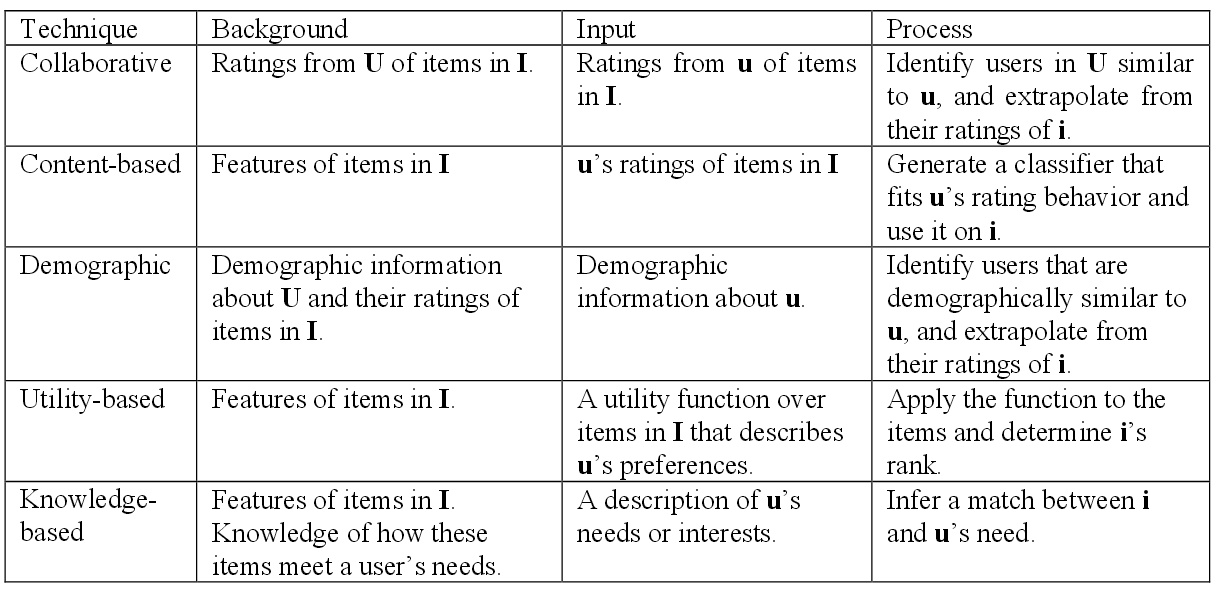
\includegraphics[width=1\linewidth]{images/types_recommandation.png}
	\caption{Techniques de recommandations [R. Burke, 2002] \cite{Burk02} }
	\label{types_recommandation}
\end{figure}    
avec :
\begin{itemize}
	\item I : ensemble d’objets sur lequel sont faites les recommandations
	\item U : l’ensemble d’utilisateurs dont les préférences sont connues
	\item u : l’utilisateur pour lequel les recommandations doivent être générées
	\item i : objets pour lesquels on souhaiterait prédire une préférence de la part de u
\end{itemize} 

		\paragraph{\emph{Collaborative} \\ \quad}
Méthode la plus mature et répandue. Le système agrège les notes ou recommandations des objets, relève les similarités entre les appréciations des utilisateurs et en déduit de nouvelles recommandations pour les utilisateurs. Certains systèmes prennent le temps en paramètre dans leur évaluation afin de prendre en compte l’évolution de l’intérêt des utilisateurs au fil du temps (effet de mode, etc). L’évaluation peut être simplement binaire ou plus complexe en utilisant une échelle de graduation. Les systèmes peuvent être soit basés sur une mémoire, comparant les utilisateurs par corrélation ou autre, soit basés sur un modèle :  celui-ci est dérivé à partir de l'historique des données d'évaluation et utilisé pour faire les prédictions.
La plus grande force de ces techniques est qu’elles sont complètement indépendantes de la représentation informatique des objets recommandés.

		\paragraph{\emph{Démographique} \\ \quad}
Ces systèmes de recommandation ont pour but de catégoriser l’utilisateur à partir de ses caractéristiques propres et de faire des recommandations en fonction de son appartenance à l’une des classes démographiques prédéfinies. L’avantage d’une approche démographique est qu’elle ne requiert pas un historique des évaluations des utilisateurs à l’inverse des méthodes collaboratives et basées sur le contenu.

		\paragraph{\emph{Basée sur le contenu} \\ \quad}
 La recommandation basée sur le contenu est une excroissance et la poursuite de la recherche d'information de filtrage. Dans ces systèmes, les objets sont définis en fonction de leurs caractéristiques associées. Le système apprend à connaître le profil de l’utilisateur en se basant sur les caractéristiques des objets évalués par l’utilisateur. C’est une corrélation objet-à-objet. Le profil dérivé dépend évidemment du type d’apprentissage employé : arbre de décisions, réseaux de neurones et représentations par vecteurs sont utilisés.

		\paragraph{\emph{Fondée sur l’utilité} \\ \quad}
Ces systèmes font des suggestions en se basant sur une estimation de l’utilité de chaque objet pour l’utilisateur. Le problème central étant comment créer cette fonction d’utilité pour chaque utilisateur. D’abord évaluer les objets (différentes méthodes), puis le profil utilisateur, avant de calculer la correspondance entre les deux. L’avantage de la technique est qu’elle peut prendre en compte des attributs non directement propres aux objets évalués (fiabilité du vendeur, disponibilité du produit, etc.) pour proposer des recommandations plus pertinentes (besoin immédiat ou meilleur prix par ex.).

		\paragraph{\emph{Basée sur le savoir/connaissance} \\ \quad}
Tenter de recommander des objets en inférant les besoins et préférences de l’utilisateur. Ces systèmes se distinguent en ce qu’ils ont un savoir fonctionnel : ils ont connaissance que tel objet répond à tel besoin et peuvent alors abstraire la relation entre le besoin et une possible recommandation.

	\paragraph{}
Les systèmes de recommandations basés sur l’utilité et sur le savoir n’essaient pas de construire des généralisations à long terme à propos de leurs utilisateurs, mais préfèrent baser leurs conseils sur une évaluation de la correspondance entre les besoins d’un utilisateur et un ensemble d’options disponibles.


	\subsection{Méthodologies de conception}
On peut naïvement imaginer deux approches de conception s’opposant dans la conception des jeux sérieux. La première consisterait, de partir des objectifs sérieux et de proposer une “gamification” de ceux-ci en ajoutant des éléments de jeu. La seconde, à l’inverse, serait de partir de la composante ludique du jeu pour y intégrer ensuite le contenu sérieux. Bien qu’ayant l’avantage d’être simples à concevoir, ces deux démarches ont pour limite d’avantager l’une ou l’autre des composantes. Un jeu sérieux conçu à partir d’une base ludique aurait un impact sérieux limité, alors que l’ajout d’une composante ludique à une finalité sérieuse serait peu convaincant.
Une troisième approche est donc de prendre en considération à la fois la composante ludique et l’intention sérieuse dès le début du processus de conception pour les fusionner au mieux. Si elle est correctement mise en place, cette approche promet une forte utilisation du jeu et un impact sérieux efficace. Elle présente néanmoins le défaut de devoir imaginer une nouvelle solution pour tout nouveau couple (jeu, objectif sérieux). C’est ce type d’approche que nous proposons ici, et nous verrons comment les résultats peuvent être réemployables.

	\subsubsection*{Participative design : conception participative}
La conception participative est une méthode de travail utilisée principalement en conception de logiciel interactif. Sa principale caractéristique est la participation active des utilisateurs au travail de conception. Il s'agit donc d'une méthode de conception centrée sur l'utilisateur où l'accent est mis sur le rôle actif des utilisateurs \cite{wiki:cp}.

\paragraph{}
Il existe dans la littérature de nombreuses variantes de la méthode et de nombreuses techniques utilisées pour impliquer efficacement les utilisateurs. On peut noter particulièrement~:
\begin{itemize}
    \item l'observation et entretiens
    \item la production de scénarios
    \item le brainstorming
    \item le prototypage papier
    \item le prototypage vidéo
\end{itemize}

\paragraph{}
Une première séance de conception a lieu en début de projet : celle-ci regroupe les chercheurs et les développeurs de l'application, mais aussi les utilisateurs futurs ou potentiels. Intégrer les utilisateurs au processus de conception permet d'entrevoir au mieux leurs besoins et d'éviter un maximum d'erreurs d'interprétation ou d'oublis (voir illustration figure \ref{projet_info}). Les utilisateurs aident aussi à définir les problèmes éventuels et leurs possibles solutions.
\begin{figure}
	\centering
	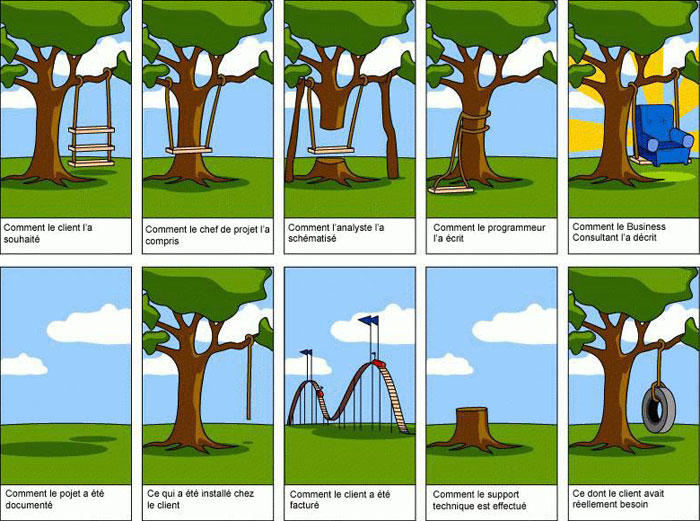
\includegraphics[width=16cm]{images/projet_info.jpg}
	\caption{Allégorie d'un projet informatique}
	\label{projet_info}
\end{figure}

\paragraph{}Par ailleurs, plusieurs séances peuvent avoir lieues tout au long du projet, afin de vérifier si les besoins ont évolués et si le développement actuel est effectivement en accord avec ceux-ci. Les utilisateurs aideront aussi l'équipe de recherche et développement à juger de la pertinence des solutions apportées.
\paragraph{}
D'un point de vue du développement, on notera que ce type de conception s'accorde parfaitement avec une méthodologie AGILE, et notamment la méthode SCRUM qui consiste en de courtes périodes de développement entre lesquelles on met en relief l'avancement par rapport au projet global.

	
	\newpage
	\section{État de l'art}
	%NaturalPad est une société innovante dont le domaine d'activité est encore à ses débuts. Si les jeux vidéo sérieux commencent à être connus du grand public et leur impact reconnu, ceux pour la santé ne sont pas encore assez nombreux ni assez largement acceptés. Mon travail de stage s'inscrit en réponse à cette constatation : il s'agit de proposer une méthode de conception de jeux vidéo pour la santé qui permettrait une simplification ou une amélioration de la conception de tels jeux. Proposer plus de jeux  thérapeutiques et/ou des jeux avec un impact santé de plus grande qualité contribuerait à améliorer leur diffusion et leur reconnaissance. Pour ces raisons, il était ainsi primordial de parfaire ma connaissance des différents domaines concernés.

Cette partie présente le résultat de mes recherches, des techniques et outils existants et comporte des notions importantes à connaître pour la conception de serious games pour la santé.

\subsection*{Méthode de travail}
Étendue sur plusieurs semaines, la réalisation de l'état de l'art était pour moi quelque chose de nouveau qui a nécessité une certaine organisation. Deux moments ont été importants : la phase de démarrage et l'arrêt des recherches. Commencer ces recherches alors que les sujets que je devais ou voulais couvrir étaient vastes et non clairement définis fut à la fois plaisant et compliqué. Bien que beaucoup de choses me semblaient intéressantes, la question était de savoir par où commencer. De la même manière, au fil de mes lectures, je découvrais de nouveaux liens et références présentant de nouveaux aspects qui eux-même renvoyaient vers d'autres solutions et articles. La difficulté était donc de juger quand mes connaissances sur un thème donné étaient suffisantes pour éviter de poursuivre d'interminables recherches, aussi intéressantes puissent elles être, le temps étant limité dans le cadre d'un stage de Master.
	\paragraph{}Au niveau des lectures abordées, ma source principale fut des articles scientifiques, suivie par des articles de magazines spécialisés et articles web notamment. Pour les thèmes médicaux, un certain nombre d'articles m'a été directement conseillé par des professionnels de la santé, articles à partir desquels j'ai ensuite pu compléter mon état de l'art en suivant les références. Par ailleurs, il est fréquent que certains auteurs ressortent régulièrement lorsqu'on effectue des recherches sur un thème donné, ce qui permet, en plus du nombre de citations des articles, de rapidement cerner quels sont les articles et chercheurs de référence dans le domaine.
	\paragraph{}Bien entendu, afin de rendre mes lectures efficaces, je me constituais pour chacune d'elle une fiche de lecture où noter les points importants : 
\begin{itemize}
	\item Titre ou source
	\item Auteur(s)
	\item Mots clefs
	\item Synthèse
	\item Jugement personnel ou remarques
	\item Références importantes
\end{itemize}

%% PART 1 : JEUX VIDEO
\subsection{Jeux Vidéo}
Durant mon stage, j'ai ainsi voulu comprendre pourquoi et comment un jeu vidéo est bon, quels en sont les mécanismes ou bien encore quels facteurs vont retenir le joueur. 

	%% Jeux vidéo et schéma comportementaux
	\subsubsection{Jeux vidéo et schémas comportementaux}
Pour expliquer l'attrait croissant de la population envers les jeux vidéo, il peut être intéressant de se tourner du coté des théories comportementales. Carl Rocray \cite{Rocr09} explique qu'en dépit de ses origines technologiques récentes, le jeu vidéo entretient d’anciens schémas de comportements, et cette influence est subtile. C’est le propre du jeu de nous divertir, non seulement de nos tracas réels, mais aussi de son influence sur nous pendant que nous jouons. Cette influence est évidente à travers le lien entre plaisir et apprentissage : l’effort diminue si on a du plaisir à le faire, et on peut même en oublier que nous apprenons.

\paragraph{}On se rend compte que la plupart des jeux vidéo peuvent être classés selon leur gameplay en ce que l'on appelle des types de jeux. Parmi les grands types connus, on retrouve par exemple les jeux d'action, les jeux de stratégie ou encore les jeux de simulation sportive. On trouvera en \href{types_jeux}{annexe} une liste plus complète de ces types de jeux vidéo classés en fonction de leur gameplay. \\

Il est intéressant de constater le lien entre les différents schémas comportementaux basiques et les types de jeux mettant en place des mécaniques stimulant nos instincts primaires [Rocray, 09]\cite{Rocr09}.

\paragraph{}
		\paragraph{Survie \\ \quad}
«Éliminer ou être éliminé». C’est la base de la majorité des jeux vidéo et probablement aussi le comportement le plus simple. Même les jeux de sports ou de cartes entretiennent cet instinct primaire, bien qu’il soit surtout manifeste dans les jeux de tir (\emph{Doom}, \emph{Gears of War}), les jeux de combats (\emph{Tekken}, \emph{Street Fighter}) et les «platformers» (\emph{Mario Bros}, \emph{Assassin’s Creed}).
		\paragraph{Gestion \\ \quad}
Il s’agit surtout de gestion de ressources, mais aussi d’équipement quand celui-ci est limité. Une bonne gestion permet habituellement de mieux survivre (meilleures ressources, équipement adéquat), ce qui nécessite une planification et une organisation stratégiques. On retrouve ce comportement dans les jeux de simulation (\emph{SimCity}, \emph{Civilization}), de «Real Time Strategy» (\emph{Warcraft}, \emph{Starcraft}) et ceux qui visent un certain réalisme (\emph{Arma}, équipement limité dans \emph{Resident Evil}).
		\paragraph{Responsabilisation d’autrui \\ \quad}
Ce comportement fait appel à une sorte d’instinct parental où nous devons assurer la survie d’un autre joueur ou le bien-être d’un avatar virtuel qui nous ramène en fait à nous-même. Il est d’abord présent dans les jeux de simulation (\emph{The Sims}, \emph{Tamagotchi}) et ceux de coopération (\emph{Army of Two}, \emph{Left 4 Dead}).
		\paragraph{Résolution de puzzles \\ \quad}
Mystères à résoudre (\emph{Myst}), problèmes de logique faisant appel à nos capacités cognitives (\emph{Brain Challenge}), voire comment empiler des formes (\emph{Tetris}) ou aligner des couleurs (\emph{Bejeweled}), il s’agit toujours de trouver la solution la plus efficace à un problème donné.
		\paragraph{Réflexes et dextérité \\ \quad}
La plupart des jeux font appel à cet instinct également lié à la survie.
Surtout lié à la coordination «oeil-main» et à la précision d’actions souvent rapides (voir entre autres les «Quick-Time Events»), il est aussi lié à la maîtrise d’un outil, c’est-à-dire la manette de jeu. On le retrouve dans les jeux de rythme (\emph{Guitar Hero}, \emph{Rock Band}), mais aussi dans les jeux de Survie cités plus haut et tous les jeux de sports.
		\paragraph{Système de récompenses \\ \quad}
La grande majorité des jeux vidéo utilise ce système de la carotte au bout du bâton pour diriger les actions du joueur. Il est donc étroitement lié à la motivation et à la gratification de comportements donnés. Voir entre autres \emph{Little Big Planet} et \emph{Diablo}, ainsi que la mode assez récente des Trophées, Succès et autres «Achievements».
		\paragraph{Système d’améliorations \\ \quad}
Une autre mécanique liée à la Survie et à la courbe de difficulté des jeux. En bref, il s’agit de devenir plus fort pour défaire des adversaires toujours plus forts. C’est la base des «Role-Playing Games» (\emph{World of Warcraft}, \emph{The Elder Scrolls}) et de certains jeux de «Shooter» (pour améliorer ses armes).

		\paragraph{}
Il est probable que d’autres comportements soient ainsi entretenus par le médium vidéo-ludique. Les sept types de mécaniques décrites ci-haut montrent néanmoins comment les jeux vidéo nous font répéter d’anciens schémas de comportement.

		\subsubsection*{Autres aspects du comportement pour la motivation du joueur}
			\paragraph{\emph{Conditionnement} \\ \quad}
Un autre aspect du jeu vidéo est sa capacité à encadrer, voir conditionner, le joueur pour lui donner envie de continuer à jouer (Voir la théorie du conditionnement par Pavlov). Bien sur, en règle générale, on cherche à ce que le joueur joue pour le plaisir, et non dans un quelconque but de conditionnement. Pour cela, le jeu va soumettre le joueur à un ensemble de stimuli de récompenses (incrémentation du score, gain d’un bonus, débloquer un niveau, feedback, etc.) lorsqu’il réalise une action positive, ou de punition (baisse du score, perte du niveau, de points de vie, etc.) lors d’erreurs. En choisissant ces ensembles de stimuli positifs et négatifs, on réussit à faire accomplir intuitivement aux joueurs ce que l’on espère qu’ils fassent.

\paragraph{}
Ces ensembles de stimuli constituent une sorte de récompenses à l’accomplissement des différentes actions du joueur. Les règles du Game Design nous enseignent qu’un jeu vidéo est constitué d’un ensemble de boucles de jeu situées à trois niveaux : micro (scène), moyen (scène et level) et macro (jeu). Ce sont les boucles OCR+M : Objective, Challenge, Reward et Means.
\begin{itemize}
	\item Objectif : état qui décide si la boucle est terminée ou non
	\item Challenge : pourquoi le joueur ne peut pas atteindre directement l’objectif
	\item Reward : récompense donnée au joueur une fois l’objectif atteint
	\item Means : moyens mis à disposition pour atteindre l’objectif
\end{itemize}
La mise en place d’objectifs a donc lieu a trois niveaux afin de toujours garder la motivation du joueur.

\paragraph{}
Plutôt que de parler de conditionnement, on peut plutôt d’association d’idées, concept sur lequel se base le conditionnement simple. Le jeu ne cherche en effet qu’à guider le joueur dans le but de le rendre autonome en lui apprenant les règles qui régissent son gameplay. Plutôt que de dire explicitement l’impact de chaque action, le jeu va souvent faire sentir au joueur ou lui faire comprendre l’impact de celle-ci, notamment par le biais des feedbacks. Libre au joueur de s’adapter ou non, sa marge de liberté étant différente d’un jeu à l’autre.\\
Un jeu comme Pong associe directement le fait de rater une balle avec celui de donner un point à l’adversaire (et donc de rapprocher le joueur de la défaite) alors que renvoyer la balle et passer l’adversaire sera clairement montré comme une action positive. Bien qu’il reste libre de ne pas chercher à renvoyer les balles et tromper l’adversaire, sa marge de liberté reste cependant limitée par le potentiel d’action et les règles du jeu : il pourra par exemple essayer de faire durer l’échange le plus longtemps possible ou chercher à ne gagner qu’avec un seul point d’avance, mais n’obtiendra aucune récompense pour cela de la part du jeu, qui n’a pas pensé à cette association d’idées. A l’inverse un jeu plus riche comme Fable ou Minecraft sera beaucoup moins binaire qu’un simple “bien / pas bien”.

	%%State of Flow
	\subsubsection{L'état de flux ou expérience optimale}
Le state of flow ou état de flux, fut originellement décrit par Csikszentmihalyi\cite{Csik88} dans les années 80 bien qu'il utilisa déjà ce terme dans ses recherches précédentes\cite{Csik75}. C'est l'état dans lequel une personne peut se trouver, proche de l’extase (dans le sens “se trouver à coté de”) complètement immergée dans ce qu'elle fait, dans un état maximal de concentration. Cette personne éprouve alors un sentiment d'engagement total et de réussite. Dans cet état, on est alors hyper compétent, naturellement, inconsciemment dans ce qu’on est en train de faire : musique, sport, travail, jeux, lecture, etc. Cet état est commun chez les personnes exerçant une activité répétitive et/ou demandant de gros efforts physiques ou psychiques. On est comme détaché de son corps, que l’on voit agir tout seul. On est alors capable d’accomplir des choses qu’on serait incapable de réaliser consciemment de manière contrôlée. S’il n’est pas interrompu, cet état d'expérience optimale peut durer une dizaine ou une vingtaine de minutes.

\paragraph{}
L’état de flux est l’une des raisons pour lesquelles on joue aux vidéo [Murphy, 2011]\cite{Murp11}. Leur but est de divertir en jouant sur la motivation du joueur, ce qui est lié au flow state. Le jeu, au moyen d’une balance entre compétences et challenge, maintient la vivacité d’esprit du joueur, avec une motivation importante et une attention forte[Rutledge, 2012]\cite{Rutl12}. Être dans cet état de flux permet donc au joueur une meilleure expérience de jeu augmentant son ressenti et son souhait de continuer à jouer[Chen, 07]\cite{Chen07}. Pour rentrer dans cet état de grâce, les deux états d’esprit les plus proches sont l’excitation et le contrôle, le flow state se trouvant à l’intersection de ces deux noeuds. On peut donc essayer de mettre le joueur dans ces états là si on cherche à stimuler ce flow state.

\begin{figure}[h!]
	\centering
	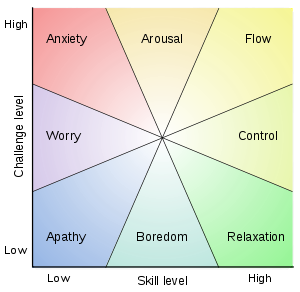
\includegraphics[width=9cm]{images/state_of_flow.png}
	\caption{Positionnement entre les humeurs et l'état de flux [Csikszentmihalyi, 1997]\cite{Csik97}}
	\label{state_of_flow}
\end{figure}

\paragraph{}
Csikszentmihalyi identifie les caractéristiques de l’état de flux~:
\begin{enumerate}
   \item prédispositions ou caractéristiques propices pour atteindre cet état~:
         \begin{itemize}
            \item des objectifs clairs et précis
            \item équilibre entre difficulté de la tâche et compétences de l’acteur (joueur)
            \item l’activité est en soi une source de satisfaction (amusante ou pour laquelle le joueur est impliquée)
         \end{itemize}
   \item conséquences et caractéristiques~:
   	\begin{itemize}
            \item hyperfocus, concentration exacerbée sur une action précise
            \item perte de la conscience de soi
            \item perception du temps modifiée
            \item rétroaction immédiate : prise de conscience de l’action effectuée, pour ajuster les suivantes
            \item sentiment de contrôle de la situation
	\end{itemize}
\end{enumerate}
	%% PART 2 : SERIOUS GAMES
\subsection{Les Serious Games}
Les serious games ou jeux sérieux sont donc une catégorie de jeux ayant la particularité d'avoir une portée supplémentaire au divertissement. Ils restent cependant des jeux en ce qu'ils en intégrent les caractéristiques ludiques, et même plus les utilisent pour parvenir plus aisément ou efficacement à leur objectif sérieux. Dans cette partie, nous allons voir comment un jeu sérieux  peut parvenir à des résultats sérieux et quels sont les mécanismes sous-jacents qui permettent une telle efficacité, souvent inconsciente chez le joueur.
	%% A Serious Games et Théories Comportementales 
	\subsubsection{Serious Games et Théories Comportementales }
			\paragraph{}
Les jeux vidéo sérieux se présentent comme un potentiel médiateur dans la modification des habitudes comportementales en permettant d’inclure des connaissances pratiques dans un modèle ludique apprécié. Il est possible d’y mettre en place des procédures de changement comme l’établissement d’objectifs ou la modélisation et le développement de compétences dans un environnement attrayant, significatif et immersif [Baranowski et al, 2008]\cite{Bara08}. \\
Les jeux vidéo promeuvent les interactions sociales et d’apprentissage [Wideman et all, 2008], créent un environnement où les actions du joueur ont un effet [Gee, 2004]\cite{Gee04} , encouragent la résolution de problèmes [Gee, 2004]\cite{Gee04} et renforcent la compréhension en créant des situations de réflexion ou en aidant le joueur dans ses objectifs [Gee, 2004]\cite{Gee04}. Enfin, les jeux sérieux pour la santé sont fait pour distraire le joueur tout en l’éduquant, en l’entrainant ou en changeant ses comportements [Stokes, 2005]\cite{Stok05}.

		\subsubsection*{Théories comportementales}
Le comportement est la résultante d’influences multiples, rendant ainsi souvent les personnes réfractaires au changement [Baranowski, Lin \& al, 1997]\cite{Bara97}. Le comportement doit alors être considéré comme un mécanisme complexe découlant de l’enchaînement de plusieurs étapes. Ainsi, plutôt que de chercher à impacter directement le comportement, les experts comportementaux valorisent une action sur ces facteurs intermédiaires, appelés médiateurs. Changer ces médiateurs permet de changer le comportement [Baranowski, Lin \& al 1997]\cite{Bara97}.
\paragraph{}Plusieurs grandes théories comportementales existent~:
\begin{itemize}
	\item la théorie d’inoculation comportementale [McGuire, 1961]
	\item la théorie socio-cognitive [Bandura, 1986]
	\item la théorie de l’auto-détermination [Ryan \& Deci, 2000]
	\item la théorie de l’immersion [Green \& Brock, 2000]
\end{itemize}

\paragraph{}De ces théories, l’on peut alors identifier un certains nombre de ces facteurs médiateurs tels que : l’immersion, l’attention, l’auto-régulation, le développement de compétences, la motivation interne et externe, l’autonomie ou encore le sentiment de compétence. La science du comportement fournit aussi des techniques qui facilitent le changement comportemental, et propose d’utiliser ces facteurs dans les média de divertissement tel que le jeu vidéo.\\
Le modèle : "Elaboration Likelihood Model" [Petty \& Cacioppo, 1986] soutient ainsi que des personnages crédibles, attrayants et sympathiques sont plus susceptibles d’être persuasifs que les autres et peuvent donc servir d’intermédiaires pour véhiculer un message. \\
La théorie d’inoculation comportementale [McGuire, 1961] met en garde contre une possible contre-productivité en identifiant et en réfutant les menaces potentielles à l’accomplissement des objectifs du changement désiré.\\
La théorie socio-cognitive [Bandura, 1986] préconise l’établissement d’objectifs et le développement de compétences comme paramètres importants dans le changement comportemental.\\
Enfin, les théories socio-cognitive [Bandura, 1986] et d’auto-détermination [Ryan \& Deci, 2000] mettent toutes deux l’accent sur l’importance du feedback pour guider et mettre en forme le comportement durant le processus de changement.	

		\subsubsection*{Théories comportementales dans un serious game éducatif}
			\paragraph{Identification \\ \quad}
Fait référence aux feedbacks ou aux conseils qui sont \emph{personnalisés} afin de mieux toucher le joueur [Kreuter, Strecher \& Glassman, 1999]. 
			\paragraph{Mini-jeux de connaissances \\ \quad}
Des connaissances pratiques et théoriques spécifiques sont un élément nécessaire, mais pas suffisant, d’une modification des habitudes comportementales [Bandura, 1986]. Ces mini-jeux peuvent être explicites (dans un mode à part) ou correspondrent aux boucles micro du gameplay.
			\paragraph{Ajustement des objectifs \\ \quad}
C’est un processus complexe qui permet à la fois de définir un objectif et les manières de l’atteindre [Gollwitzer, 1999], en prenant en considération les capacités et valeurs personnelles pour les lier à son objectif [Ryan \& Deci, 2000]. Parce que l’autonomie améliore la motivation personnelle [Ryan \& Deci, 2000], proposer et permettre au joueur de réaliser ses propres choix ou de paramétrer ses objectifs est donc conseillé.
			\paragraph{Résolution de problèmes \\ \quad}
Bien que les difficultés et obstacles interfèrent de premier abord dans la réalisation de ses objectifs, arriver à les surmonter est un moteur de motivation puissant [Frauenknecht \& Black, 1995]. Le joueur doit prévoir ces difficultés et mettre en place un plan pour arriver à les dépasser. Ces solutions doivent paraitre réalisables et plausibles pour ne pas décourager le joueur [Elaboration Likelihood Model : Petty \& Cacioppo, 1986].
			\paragraph{Exposition des motivations \\ \quad}
La théorie de l’auto-détermination [Ryan \& Deci, 2000] indique que la motivation personnelle est d’autant plus importante que la personne voit le lien entre son comportement et des choses importantes pour elle, comme une valeur qui lui est chère. Par exemple dans un serious game de rééducation motrice, si pouvoir faire du tennis est une chose importante pour le joueur-patient, on lui rappellera que réaliser des étirements quotidient permet de récupérer plus rapidement.
			\paragraph{Revue des objectifs et du travail accompli\\ \quad}
Cette activité renforce le sentiment d’accomplissement personnel et augmente l’auto-efficacité [Bandura, 1986].
			\paragraph{Feedback \\ \quad}
Un feedback bien conçu renforce l’efficacité personnelle [Schuk, 1986] et le sentiment de compétence. [Ryan \& Deci, 2000]
			
\paragraph{}
Pour vérifier l'application de ces théories sur un cas pratique, [Thompson et al, 09] ont participé à la création d'un Serious Game~: DIAB. DIAB est un jeu vidéo divertissant, mais sérieux et se basant sur ces concepts théoriques, conçu pour réduire les risques de diabète de type 2 et d’obésité infantile. Il émerge de cette expérience que les jeux sérieux fondés sur une base théorique peuvent être efficaces pour parvenir à un changement à la fois dans le régime alimentaire et l’activité physique. Peu est encore connu dans le domaine, mais il en sort que les mécanismes et processus de changements comportementaux ont aussi leur place dans les jeux sérieux et peuvent permettre d'améliorer l'efficacité de ces derniers. Cette expérience décrit aussi comment des experts du divertissement et d'une spécialité différente peuvent allier leurs talents respectifs pour créer un jeu sérieux efficace et divertissant basé sur un socle théorique. 
	%% Apprentissage et propriétés des jeux vidéo
	\subsubsection{Apprentissage et propriétés des jeux vidéo}
			\subsubsection*{Théories de l'apprentissage}
Les serious games sont aujourd'hui utilisés comme nouveaux vecteurs d'apprentissage. Ils sont en effet porteurs de nombreux éléments qui sont propices à l'apprentissage [Baranowski, 08]. On ne connait cependant pas la relation entre les attributs d'un jeux et les résultats de l'apprentissage, ni si ces liens sont directs ou indirects, si un seul paramètre ou une combinaison de ceux-ci auront un impact différent ou plus important [Wilson 09]\cite{Wils09}. 

\paragraph{}Plusieurs théories de l'apprentissage permettent d'en expliquer les mécanismes, que nous essaieront par la suite de lier aux paramètres d'un jeu vidéo.\\

\emph{Cognitive learning outcomes} :  Dans cette théorie, [Kraiger et all, 93] développent 3 notions : la connaissance déclarative (le quoi), la connaissance procédurale (le comment) et le savoir tacite ou stratégique (qui, quand, pourquoi). Ces trois catégories décrivent le processus cognitif d'apprentissage, et se rapprochent fortement des sous-catégories de la connaissance de [Bloom, 1956].\\ 

\emph{Skill-based learning outcomes} : En poursuivant le développement de leurs capacités cognitives, les apprenants progressent vers des méthodes d'apprentissage basées sur les compétences. Ces compétences se concentrent sur le développement de techniques ou de compétences motrices en dépassant progressivement la phase de réflexion consciente. Les compétences psychomotrices demandent de la pratique et peuvent être catégorisées parmi 7 catégories de la plus simple à la plus complexe : perception (sentir les moteurs permettant de réaliser le mouvement), volonté d'agir, imitation (être capable de réaliser un mouvement défini), automatisme(réalisation d'un schéma moteur), réponse manifeste complexe, adaptation et originalité.\\ 

\emph{Affective learning outcomes} [Kraiger et al 1993]. Selon cette théorie, l'apprentissage façonne aussi les sentiments d'un individu. Kraiger et al décrivent les résultats d'un apprentissage par les émotions comme impliquant des concepts tels que l'attitude, la motivation et les objectifs.\\

En 2012, Curtiss s'inspire des lois de l'apprentissage de Thorndike qui décrivent trois principes : la bonne volonté(readiness), la pratique(exercice) et l'effet(effect), auxquels ont été depuis ajoutées les lois de primauté, d'intensité et de récense. Son travail portant sur l'utilisation de serious games éducatifs dans l'armée, il simplifie et ne garde de ces lois que les aspects inconditionnels, dans le temps ou le milieu d'apprentissage par exemple. Il décrit ainsi six nouvelles lois de l'apprentissage pour les jeux, décrites dans le tableau de la figure \ref{laws_of_learning_for_games}.

\begin{figure}[h!]
	%\centering
	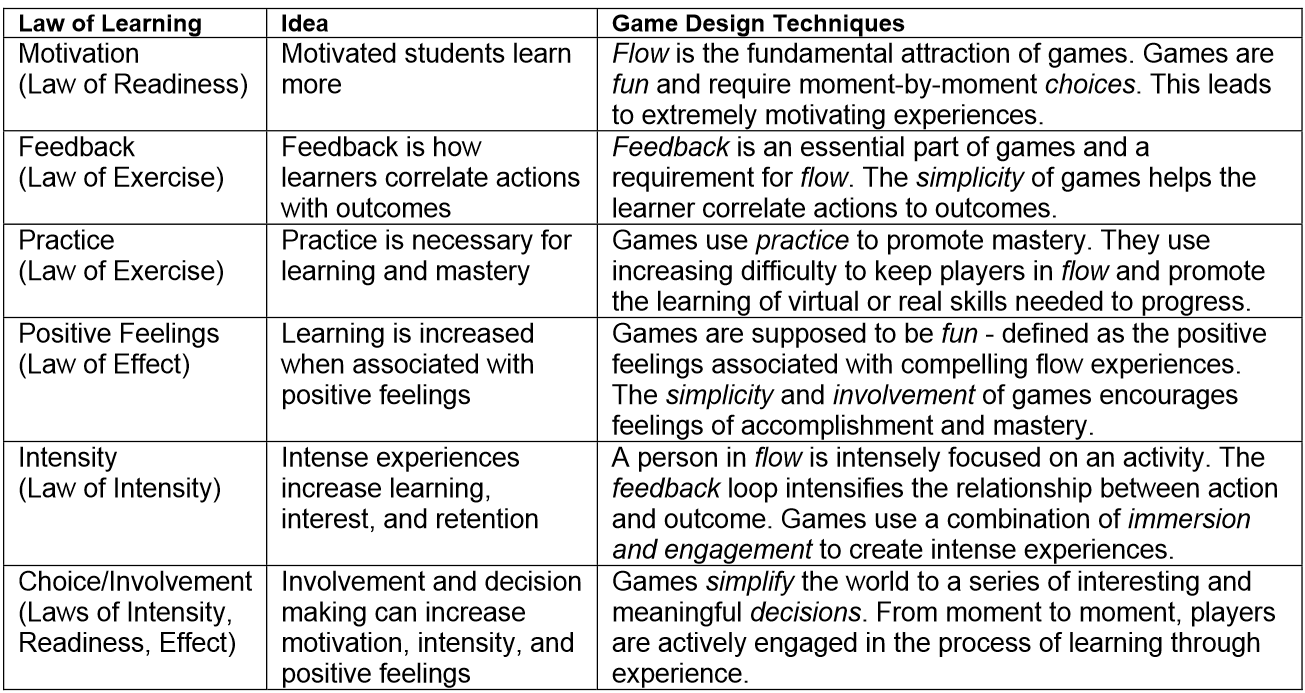
\includegraphics[width=1.1\linewidth]{images/laws_of_learning_for_games.png}
	\caption{Lois de l'apprentissage dans les jeux vidéo, [Murphy, 2011]\cite{Murp11}}
	\label{laws_of_learning_for_games}
\end{figure}

			\subsubsection*{Propriétés des jeux vidéo}
En 1984, [Driskell and Dwyer]\cite{Dris84}réalisent un premier état de l'art et trouvent que plusieurs caractéristiques des jeux vidéo peuvent influer sur les propriétés d'apprentissage et de motivation : des objectifs spécifiques, un challenge, de la fantaisie et du mystère. Ils théorisent qu'une augmentation de la motivation produit une augmentation de l'attention et mène à une meilleure mémorisation des acquis (connaissance déclarative) et une focalisation de l'attention (stratégie cognitive).\newline
[Malone et Lepper, 1987] mentionnent le challenge, la curiosité, le contrôle et la fantaisie comme caractéristiques intégrantes des jeux vidéo. Selon [de Felix et Johnson , 1993], les jeux sont composés d'éléments visuels dynamiques, d'interactions, de règles et d'objectifs. Puis [Thiagarajan, 1999] affirme que le conflit, le contrôle, la terminalité et l'artifice sont les quatre éléments nécessaires d'un jeu. En 2001, [Garis and Ahlers, 01] donnent 39 descripteurs qui seront réduits à 12 pour ne garder que les paramètres statistiquement les plus significatifs pour renforcer la sensation de "game-like". \\ Finalement en 2002, [Garris et al] proposent un sous-ensemble de tous ces attributs qui seront considérés commes les paramètres de jeu clefs de l'apprentissage~:
\begin{itemize}
	\item la fantaisie
	\item les règles
	\item la stimulation sensorielle
	\item le challenge
	\item le mystère
	\item le contrôle
\end{itemize}

\paragraph{}En 2009, [Wilson et al]\cite{Wils09} partent de l'ensemble de paramètres de [Garris et al] pour enrichir le modèle avec de nouveaux paramètres qui leur semblent avoir un impact sur l'apprentissage.
Les tableaux \ref{game_attributes_one} et \ref{game_attributes_two} indiquent et décrivent ces douze attributs.

\begin{figure}[h!]
	\centering
	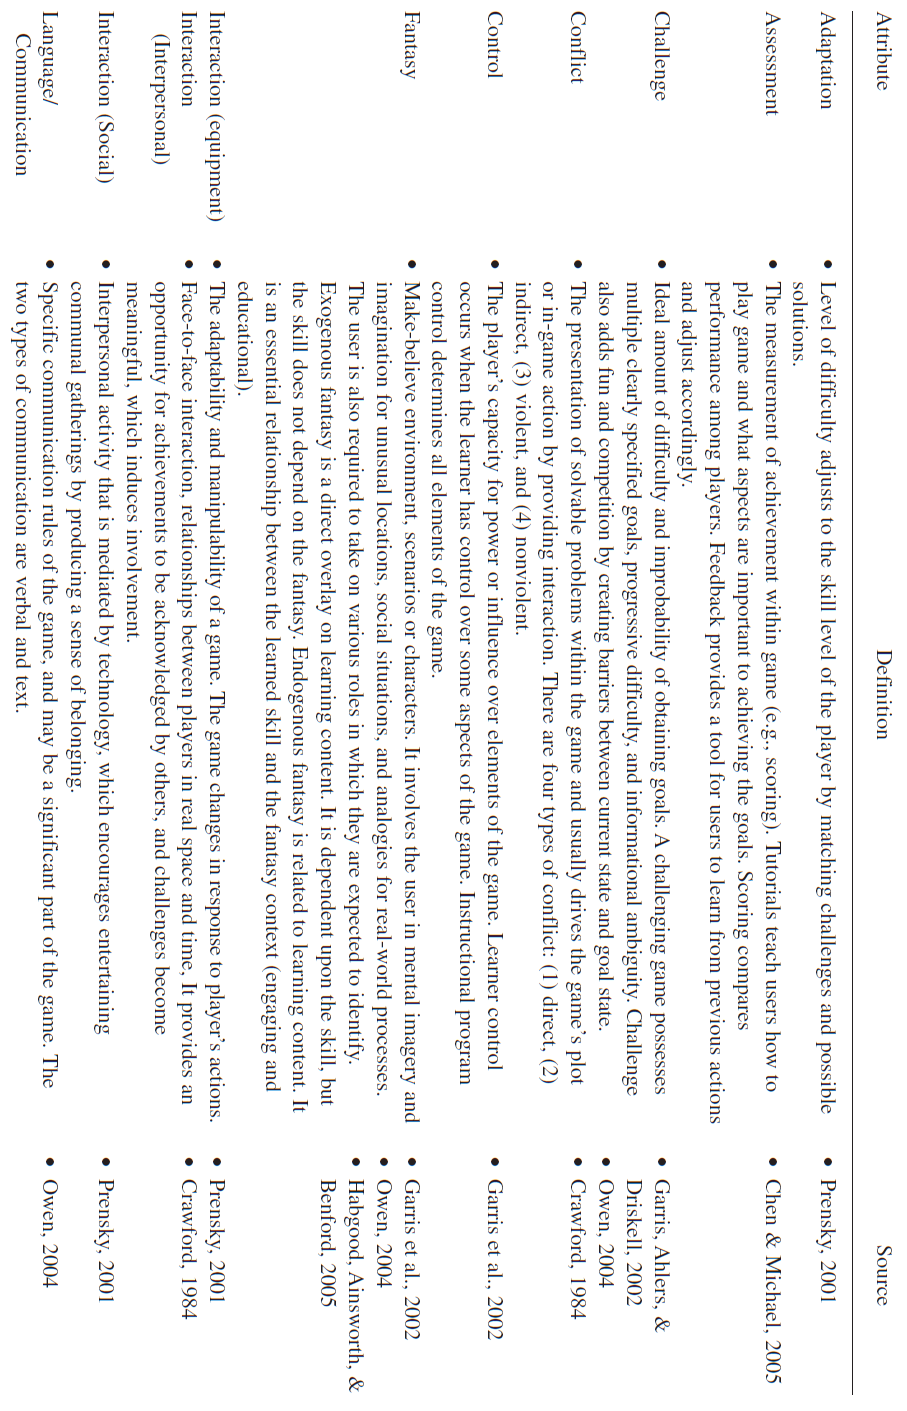
\includegraphics[width=\linewidth, height=\textheight ]{images/game_attributes_one}
	\caption{Propriétés des jeux vidéo et leur définition. (1/2) \cite{Wils09}}
	\label{game_attributes_one}
\end{figure}
\begin{figure}[h!]
	\centering
	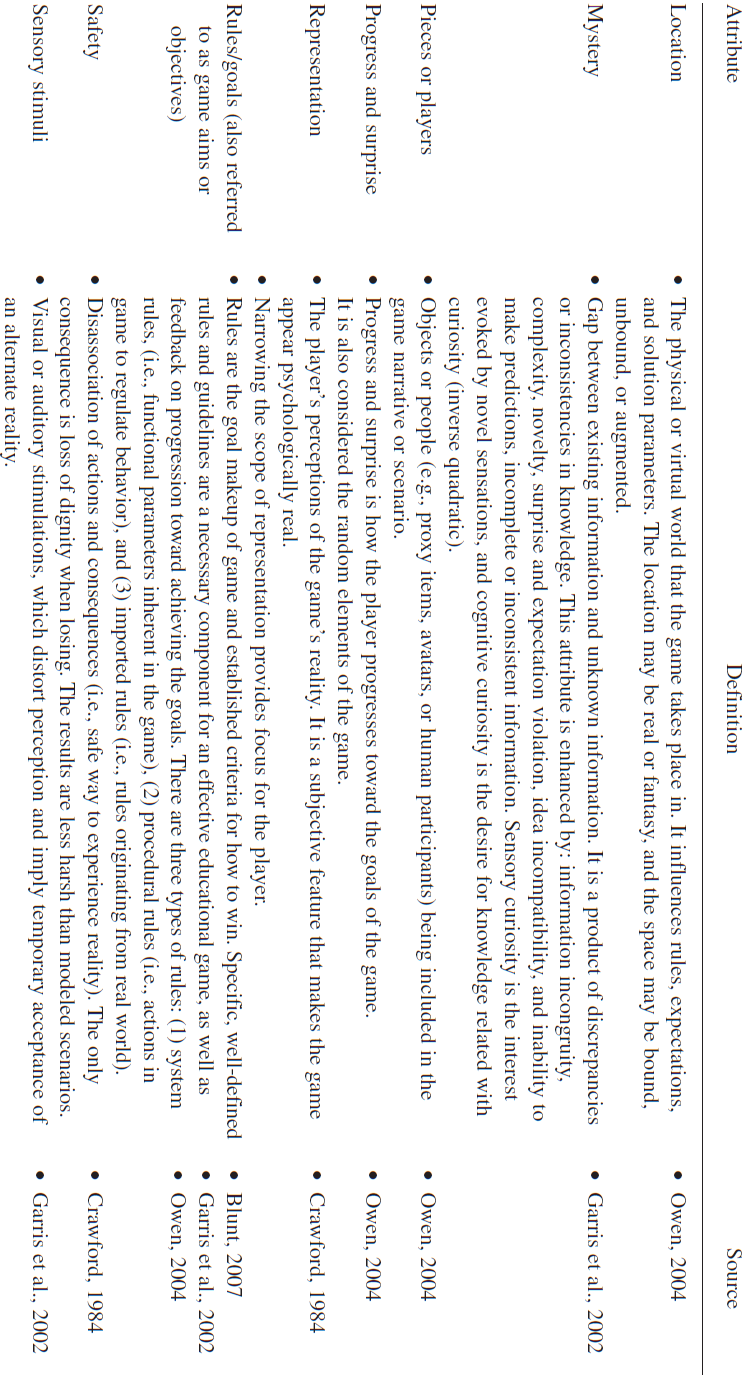
\includegraphics[width=\linewidth, height=\textheight ]{images/game_attributes_two}
	\caption{Propriétés des jeux vidéo et leur définition. (2/2) \cite{Wils09}}
	\label{game_attributes_two}
\end{figure}

		\subsubsection*{Les jeux vidéo comme outil d'apprentissage}
Les concepteurs de bons jeux vidéo mettent en place d'exellentes méthodes pour que les joueurs apprennent et aiment apprendre dans le jeu vidéo. Initialement, cet apprentissage ne concernent que les principes importants pour jouer au jeu, mais on observe très vite un phénomène d'apprentissage tangentiel chez les joueurs, qui apprennent aussi plus facilement des notions facultatives pour le gameplay. Gee se propose en 2005 de discuter de 13 principes d'apprentissage efficaces, et de leur intérêt à les mettre en application au travers de jeux vidéo. Il divises ces principes en trois catégories en précisant que le principal problème à la mise en place de tels systèmes d'apprentissage reste le coût.
			\paragraph{\emph{La participation des apprenants ( Empowered Learners)}}
			\begin{itemize}
				\item {Co-design} : l'apprenant doit être un acteur actif (producer) et non passif (consumer)
				\item {Customisation} : l'apprenant doit pouvoir prendre des décisions quant à la méthode
d'apprentissage (chacun est différent) et s'essayer (être encouragé) à de nouvelles.
				\item {Identification} : un apprentissage en profondeur requiert une réelle implication,
implication qui se fait bien plus présente lors d'un jeu de rôle
				\item {Manipulation et connaissance distribuée} : les sciences cognitives montrent que la
pratique, notamment au travers d'un tiers (robot, entité, etc) permet de ressentir soi
même les choses et de mieux les comprendre (empathie).
			\end{itemize}

			\paragraph{\emph{Résolution de problèmes}}
			\begin{itemize}
				\item {Difficulté progressive (well-ordered problems)} : être confronté trop tôt à un problème
trop difficile n'est pas efficace, bien que pouvant amener à des solutions très créatrices ;
alors qu'une évolution progressive de la difficulté permet à l'apprenant de comprendre
seul au fur et à mesure.
				\item {Frustration plaisante} : notion de challenge : dur mais faisable
				\item {Cycle d'expertise} : répéter et pratiquer ses compétences jusqu'à les maîtriser, puis
confronter l'apprenant à une difficulté lui demandant de mettre en pratique toute cette
maîtrise, ancienne ou récente. Puis répéter ce cycle à un niveau plus élevé (système
levels /boss)
				\item {Information ‘On Demand’ and ‘Just in Time’} :
On part du constat que les humains ne peuvent / veulent pas emmagasiner une grande
quantité d'information sans contexte. On apprend beaucoup mieux une information si
elle est donnée dans un cas d'utilisation, un contexte, liée à une image, etc. C'est le « just
in time ». De la même manière, on peut vouloir la retrouver aisément lorsqu'on en a
besoin, le « on demand ». Cela se traduit dans les jeux par les tutoriels et manuelsd'utilisation.
				\item {Aquarium} : C'est le principe de l'écosystème simplifié permettant d'appréhender un sous
ensemble des paramètres, afin de ne pas être directement surchargé par la masse
d'information. Jeux-> version démo ou premiers niveaux simplifiés (didacticiels)
				\item {Sandboxes :ou Bac à sable} : proposer un environnement identique à l'environnement
réel, mais plus sur et sécurisé. Dans ce contexte, l'apprenant va pouvoir expérimenter
sans risque avec un réel sentiment d'accomplissement et d'authenticité.
Il n'y a rien de pire qu'un jeu où après bien des efforts, on perd juste avant de pouvoir
sauver. Cela induit une manière de jouer très 'safe' où ne prend plus aucun risque sans
chercher à explorer les possibilités du jeu.
				\item {Skills as Strategies} : Sur le principe de « c'est en forgeant que l'on devient forgeron »,
c'est à force de pratiquer une compétence qu'on finit par la maîtriser. Mais on n'aime pas
pratiquer sans raison, il faut donc arriver à lier ses objectif perso avec l'utilisation de la
compétence. Ingame -> passer par une phase obligatoire d'utilisation d'un skill (zelda)
		\end{itemize}
			\paragraph{\emph{Compréhension}}
		\begin{itemize}
				\item {Pensée globale (System Thinking )}: Comprendre comment s'intègre la notion ou
compétence nouvelle dans le système global permet de mieux l'appréhender. Pousser
cette compréhension (en montrant quels leviers d'action permet ou non chaque
élément)de manière à être capable d'inférer les règles 'sémantiquement' liées.
				\item {Meaning as Action Image} : Le fait que quand les gens pensent à un concept, ils n'y
pensent pas à travers sa définition générale, mais à travers l'expérience personnelle qu'ils
ont de ce concept. Lié au principe « Just on time and on demand »
		\end{itemize}	

	%% Serious games thérapeutiques
	\subsubsection{Serious games pour la santé}
TODO 
\begin{figure}
TODO Succinte explication du lien entre mes composantes. Vérifier que ca se trouve avec le reste et pas en fin de document.
	\centering
	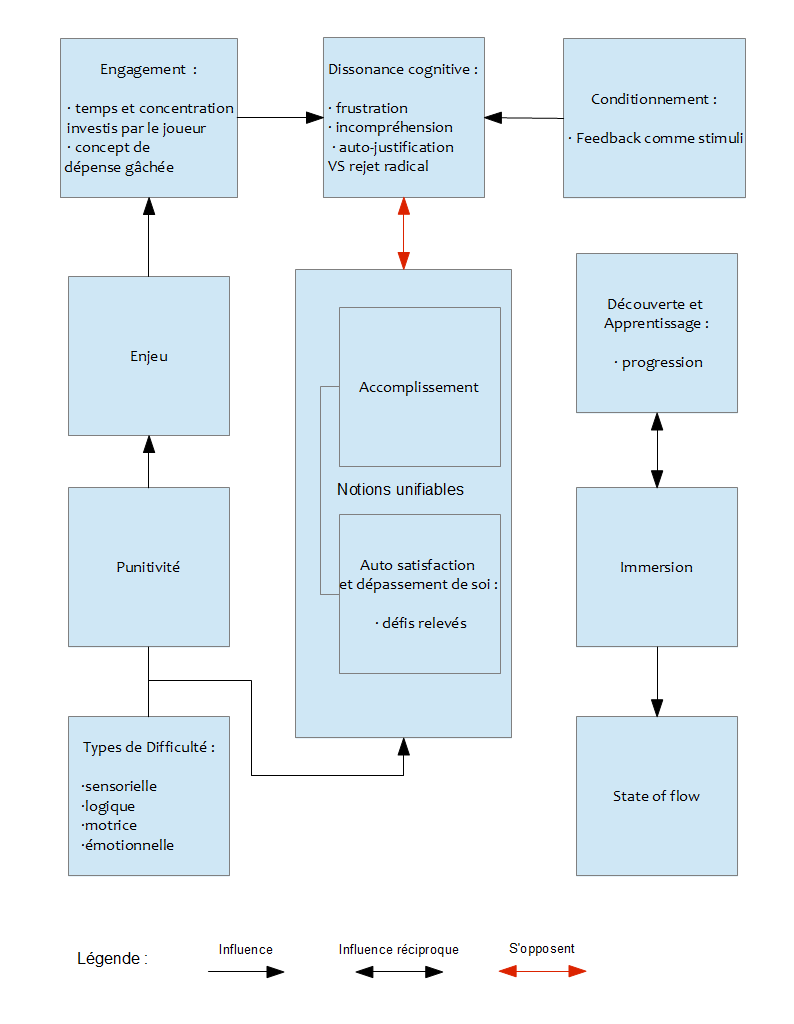
\includegraphics[height=19.6cm]{images/lien_theories}
	\caption{Relation entre les principaux ressorts psychologiques d'un jeu vidéo}
	\label{lien_theories}
\end{figure}
	\subsection{Réhabilitation et serious games pour la santé}

		\subsubsection{Adaptation de la difficulté dans une rééduc fonctionnelle aujourd'hui (exercices de récup sensorielle, de mouvements, etc)}
Existence de jeux sérieux à but thérapeutique ayant pour but de faciliter la réhabilitation en maintenant la motivation du patient. Cependant, ces jeux sont encore rares et ne remplissent pas encore parfaitement leur rôle à cause du problème de l'ajustement de la difficulté en fonction du joueur.
Or comme l'a vu, la difficulté joue un rôle important dans la satisfaction et la motivation du joueur. La question se pose donc de savoir comment ajuster de manière la difficulté d'un jeu afin qu'elle sied au mieux à chaque joueur, à chacune de ses sessions, dans le but final de renforcer la récupération motrice du joueur-patient. On va par ailleurs chercher à fournir le meilleur environnement virtuel possible pour chaque situation, avec ici comme objectif de contexte à terme un couple patient-thérapeute avec considérations des objectifs thérapeutiques. 
		
		\subsubsection{personnes âgées\\}
pas/peu d'expérience de jeu, voir même des nouvelles technologies, capacités physiques restreintes, background social à prendre en compte (jeux de cartes préférés aux jeux de guerre)
		\subsubsection{hémiplégiques\\}		
Contraintes spécifiques.
		\subsection{Ajustement de la difficulté}
Il est nécessaire d'adapter la difficulté pour chaque joueur pour garantir une expérience de jeu optimale.			
\begin{quote}Malone : “Pour être stimulant, un jeu doit proposer un but que le joueur n’est pas certain d’atteindre”.
\end{quote}

	\subsubsection{Objectifs et paramètres d'ajustement}
L’objectif de l’ajustement de la difficulté est de pouvoir faire correspondre la difficulté du jeu aux capacités et niveau de jeu du joueur, de manière à ce que quel que soit son niveau, le feedback difficulté puisse être identique. Dans leur ouvrage \emph{On Game Design} \cite{Andr03} Andrew Rollings et Ernest Adams précisent cependant que l’ajustement ne doit pas être trop évident ni visible, afin d’éviter toute forme d’exploit, évidemment non voulu. Ils précisent aussi que cet ajustement ne doit pas se faire au détriment de l’impact décisif de l’action du joueur ; celui-ci doit rester le facteur décisif de sa réussite ou non, indépendemment de l’ajustement réalisé par le système. On pourra noter qu’un niveau de difficulté idéal mènerait le joueur à un taux d’échecs/réussites de 50/50.

		\paragraph{\emph{Évaluation de la difficulté}\\ \quad}
Modifier la difficulté d'un jeu vidéo ne semble pertinent qu'après en avoir évaluer le niveau lors de phases de tests. Deux types de tests peuvent être mis en place. 
\begin{itemize}
	\item des tests de jouabilité, réalisés par des joueurs testeurs : fidèles mais couteux et complexes à mettre en place, définis dans le temps et subjectifs.
	\item des tests par joueur synthétique : rapides, peu chers et répétables mais basiques, sans perception subjective, ignorent les aspects perceptifs.
\end {itemize} 

	\paragraph{\emph{Jeux de progression VS jeux d’émergence} \\ \quad}
Les jeux de progression sont scénarisés et le level design est défini et fixé à l’avance. La difficulté y est donc statique et prédéfinie selon les choix des designers. L’ensemble des situations du jeu a été pensé et calibré. Le parcours est relativement contraint et organisé. \\
Dans les jeux émergents, on ne peut prévoir l’évolution de la partie. Seul un certain nombre de règles permet de définir et de faire évoluer le contenu du jeu par application de ces règles et de l’interaction du joueur avec les objets du jeu. \\
Progression et émergence constituent en fait les deux formes opposées d’une catégorie décrivant le contrôle que possède le level designer sur l’expérience du joueur. On remplacera alors le contrôle manuel des designer par des algorithmes de génération appropriés. Un jeu pourra ainsi se situer le long de l’axe décrivant ce contrôle selon sa conception du level design (figure \ref{axe_scenaristique}). 
\begin{figure}[hbtp]
\centering
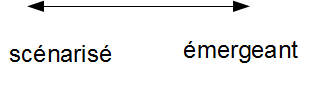
\includegraphics[width=5cm]{images/axe_scenaristique.png}
\caption{Axe scénaristique d'un jeu vidéo}
\label{axe_scenaristique}
\end{figure}

\paragraph{}Il existe un sous domaine de l’intelligence artificielle qui cherche à lier contenus émergents et scénarisés afin de tirer parti des avantages respectifs de l’un et l’autre domaine tout en limitant leurs contraintes : la narration interactive. On cherche alors à créer un univers virtuel où l’on va pouvoir “aller n’importe où et faire n’importe quoi, quand on le souhaite” de manière cohérente à la fois d’un point de vu gameplay et scénario. Cela en adaptant par exemple le scénario en fonction du comportement du joueur (utilisation par exemple d’un Drama Manager).

			\paragraph{\emph{Scénarisation VS adaptation dynamique} \\ \quad}
Le problème de l’adaptation de la difficulté est abordable à partir de deux méthodes de game design : la scénarisation et l’adaptation dynamique de la difficulté.  Ces deux méthodes pourraient bénéficier d’une méthode générale de la mesure de la difficulté, pour s’adapter au mieux.

\paragraph{}La scénarisation est une manière d’encadrer l’apprentissage du joueur à l’aide d’un découpage du gameplay en phases successives. 

\paragraph{}L’adaptation dynamique permet de maintenir le niveau de difficulté du jeu cohérent avec les capacités du joueur. Ces méthodes d’auto-adaptation peuvent être très efficaces, notamment pour ajuster un certain nombre de paramètres. Des algorithmes peuvent ainsi restreindre la lisibilité du jeu ou relâcher les contraintes de réalisation d’une action en fonction des résultats du joueur. On peut alors soit jouer sur la difficulté de la tâche ou de l’action à réaliser, soit sur les moyens employables pour y arriver (vie, temps, capacités, temps de réaction, propriétés du joueur / de l’environnement, etc.). Attention tout de même à ne pas faire un “système parfait” qui ferait que le joueur ne serait alors plus le facteur déterminant de sa réussite.

		\paragraph{\emph{Équilibrage dynamique} \\ \quad}
L’équilibrage dynamique, ou ajustement dynamique, consiste à modifier un certain nombre de paramètres du gameplay afin de s’adapter au comportement du joueur [Levieux, 11]. Il faut cependant pour cela d’abord être capable d’évaluer l’équilibre du jeu, sans quoi toute modification serait infondée . Dans cet objectif, l’apprentissage dynamique est particulièrement exploré. Ces techniques permettent en effet de calculer automatiquement les meilleurs paramètres pour atteindre un but donné, la difficulté du gameplay en l'occurrence. Idéalement, le jeu serait ainsi capable de détecter quand et comment le joueur parvient à surpasser les obstacles qui lui sont proposés, puis d’y répondre en proposant des modifications visant à obliger le joueur à reconsidérer sa stratégie de jeu. Bien sur, il est possible que le système ne parvienne pas à détecter la stratégie (voir l’exploit) du joueur, ou soit incapable de fournir une réponse appropriée ou cohérente avec l’univers du jeu, d’un point de vue autre que le gameplay pur. En effet, de tels systèmes ne prennent pas en compte l’intégralité de la pensée du game designer, qui reste complexe et non entièrement formalisable (visée artistique, morale, intentions, proposition d’une ‘expérience’ de jeu, etc.).

\paragraph{}Un jeu est donc une activité qui demande un effort au joueur. Cet effort librement consenti par le joueur  doit être utile pour la réussite ou non à ce jeu, puisqu’il pourrait aisément être rendu vain ou superflu en modifiant les règles du jeu. La difficulté, définie comme l’effort réalisé par le joueur, est donc une composante essentielle du jeu de part sa relation avec le joueur.

		\subsubsection{Techniques d'adaptation dans les jeux ludiques et sérieux}
L'adaptation de la difficulté dans les jeux vidéo est une fonctionnalité importante qui permet d’individualiser et de contextualiser l'expérience de jeu. Dans le cas de serious games, elle permet également de gérer la frustration des joueurs-apprenants tout en augmentant leurs motivations [Hocine et al 11]. L'individualisation et la contextualisation du jeu pour chaque joueur-apprenant, notions déjà définies par [Gee, 05] comme importantes pour l'apprentissage, ont pour conséquence d'augmenter sa satisfaction tout en améliorant l’efficacité de la formation.
				
		\paragraph{}
La génération dynamique d’IA permet de modifier le niveau de difficulté en créant de nouvelles entités avec un niveau et des règles donnés, ou en modifiant des paramètres du gameplay en cours de jeu.\\
Par exemple, Andrade et al utilisent l’apprentissage dynamique pour ajuster la difficulté. L’algorithme consiste à utiliser une base de couples (action, état de jeu) associés chacun à une valeur d’efficacité, afin que le jeu choisisse pour chaque situation un comportement de l’efficacité souhaitée.			
				
		\paragraph{\emph{Systèmes adaptables VS systèmes auto-adaptatifs} \\ \quad} 
L’adaptation peut être définie comme une caractéristique exprimée au niveau d’un système, dans notre cas un système informatique, qui reflète sa capacité à se modifier structurellement en réaction à certains évènements bien identifiés (Andresen K. et al, 2005). Nous parlerons de système adaptable lorsque l’intervention humaine est nécessaire pour enclencher le processus de modification et de système auto-adaptatif si aucune intervention extérieure n'est nécessaire (Moisuc B., 2001)

\paragraph{}
Levieux précise que la génération dynamique d’IA permet de modifier le niveau de difficulté en créant de nouvelles entités avec un niveau et des règles donnés, ou en modifiant des paramètres du gameplay en cours de jeu.\\
Par exemple, Andrade et al utilisent l’apprentissage dynamique pour ajuster la difficulté. L’algorithme consiste à utiliser une base de couples (action, état de jeu) associés chacun à une valeur d’efficacité, afin que le jeu choisisse pour chaque situation un comportement de l’efficacité souhaitée.

		\paragraph{\emph{Adaptation de la difficulté dans les jeux sérieux} \\ \quad}
Contribuer à l'acceptation et à l'utilisation des jeux sérieux constitue un enjeu majeur pour la réussite et l'efficacité de ceux-ci. En effet, ces systèmes sont destinés à satisfaire les joueurs-apprenants et à répondre à leurs besoins en termes d'acquisition de compétences et/ou de divertissement. L’adaptation a pour but d’améliorer l’utilisabilité d’un jeu sérieux ou ludique en restructurant certaines de ses propriétés.

\paragraph{}
[Hocine et al, 11] se proposent d'étudier les différents systèmes d'adaptation dans les jeux ludiques et sérieux. Pour évaluer ces systèmes, ils définissent trois critères majeurs :
\begin{itemize}
	\item L’efficacité d’un système évalue le degré de succès avec lequel les utilisateurs réalisent leurs objectifs dans le système.
	\item L’efficience évalue les moyens mis en œuvre par les utilisateurs pour accomplir leurs objectifs.
	\item La satisfaction évalue le niveau d’acceptation par les utilisateurs.
\end{itemize}

\paragraph{}
Afin d'évaluer et de comparer les différents systèmes, ils utilisent un système d'évaluation des techniques d'adaptation intéressant et très parlant du fait qu'il repose sur un modèle MVC (voir figure \ref{criteres_adaptation}).

\begin{figure}[!hbtp]
	\centering
	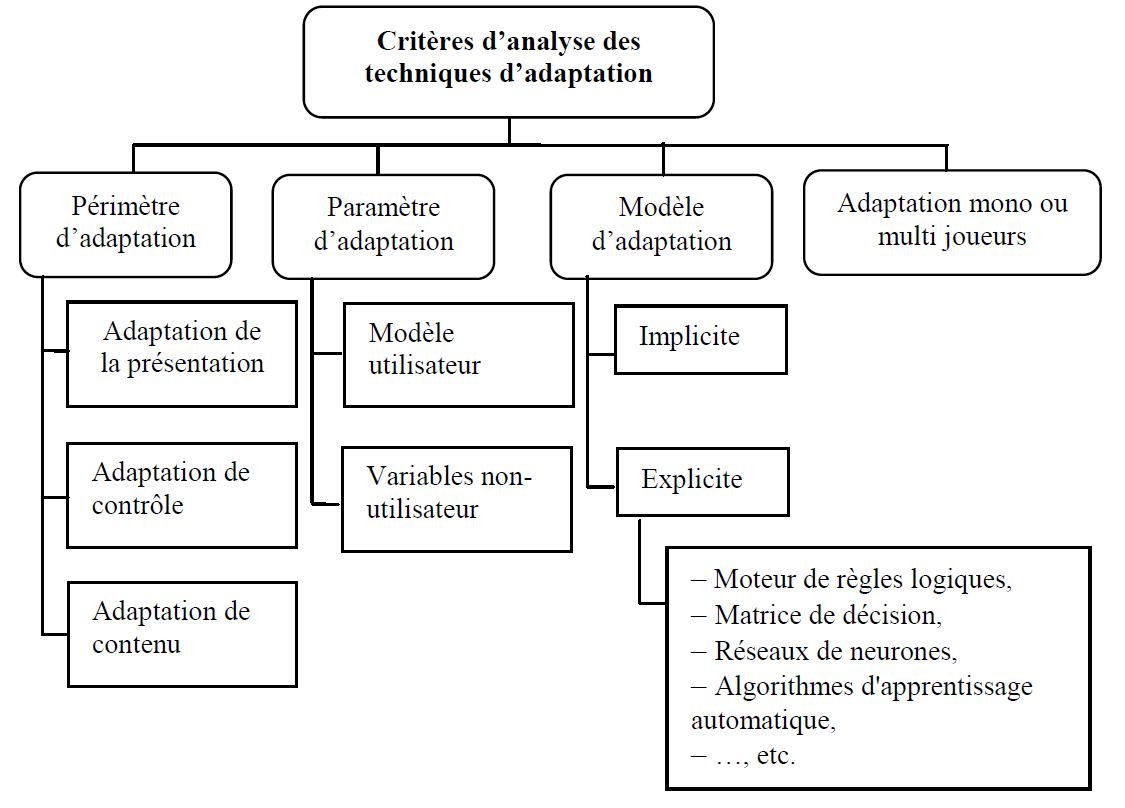
\includegraphics[width=1\linewidth]{images/criteres_adaptation.png}
	\caption{Critères d’analyse des techniques d’adaptation [Hocine et al, 2011]\cite{Hoci11}}
	\label{criteres_adaptation}
\end{figure}

	\paragraph{Périmètre d'adaptation\\}
Le périmètre de l'adaptation identifie le périmètre dans lequel l'adaptation est appliquée, selon le modèle MVC. 
\begin{itemize}
	\item \emph{Adaptation de la présentation (la Vue)}. L'adaptation peut donc avoir lieu au niveau de l'interface, du son ou de feedbacks envers l'utilisateur. Dans Hammer \& Planks, nous avons ainsi rendu possible la modification de ces paramètres : ajustement du volume de la musique ou des bruitages, contraste, taille des objets, vitesse de jeu et possibilité de désactiver les éléments cosmétiques facultatifs au jeu (animation de la mer, effets visuels etc.).
		\item  \emph{Adaptation du contrôle} : ce niveau englobe les règles du jeu et les règles métier qui spécifient la dynamique du jeu (ou le gameplay) en réaction aux actions des joueurs. C'est dans ce niveau que l'on adaptera le niveau de difficulté du jeu. Suite à mon travail sur le jeu Hammer \& Planks, il est possible de modifier le nombre et le type d'ennemis que doit affronter le joueur, la vitesse du jeu, les propriétés des personnages (joueur ou ennemis) ou encore la fréquence des obstacles par exemple.
		\item  \emph{Adaptation du contenu (le Modèle)} : l'adaptation à ce niveau modifie dynamiquement soit les schémas de données utilisés ou bien le contenu. L'adaptation s'efforce donc de produire un contenu lié au contexte de jeu et aux compétences des joueurs. Nous pouvons citer à titre d'exemple la génération automatique des dialogues et textes narratifs (Barry G., 2007) ou d'ambiance sonore (Chen Y et al, 2006)
\end{itemize} 

	\paragraph{Paramètres d'adaptation\\}
Ce sont les éléments sur lesquels repose la prise de décision du processus d'adaptation. Ces éléments vont être utilisés soit comme déclencheurs de l'adaptation soit comme sources de données. Hocine et al distinguent deux types de paramètres en fonction de l'utilisateur~:
\begin{itemize}
	\item \emph{Modèle utilisateur} : ensemble de variables et métriques décrivant les caractéristiques de l’utilisateur dans le système. Ces caractéristiques peuvent être des données représentant les préférences de l’utilisateur, son état attentionnel, ses émotions et/ou ses compétences. Ces données sont stockées dans le profil de l’utilisateur qui sera utilisé comme paramètre de processus d’adaptation.
	\item \emph{Paramètre non-utilisateur ou variable système }: ce paramètre représente les variables propres au système et qui ne dépendent pas du modèle utilisateur. A titre d'exemple, nous pouvons citer les paramètres liés à la configuration matérielle et logicielle du système hôte.
\end{itemize}

	\paragraph{Modèle d'adaptation\\}
	L’adaptation peut être implémentée dans le système sous forme d’un module qui interagit avec le système pour modifier son comportement et sa structure. Ce module peut être~:
\begin{itemize}
	\item \emph{Implicite} : dans ce cas les procédures d'adaptation se retrouvent éparpillées et étroitement liées aux différents composants du système. Il serait dans ce cas difficile de séparer dans les instructions (ou le code source) les éléments qui incombent à l'adaptation des autres aspects.
	\item \emph{Explicite }: la technique d'adaptation utilise des modèles explicites comme un moteur de règles logiques, une matrice de décision ou des algorithmes d’IA.
\end{itemize}
	
	\paragraph{Adaptation Mono ou Multi-joueurs\\}
Contrairement aux jeux mono-joueur, l'adaptation dans un système multi-joueurs doit prendre en compte l'aspect collaboratif et l'hétérogénéité entre les joueurs tout  en maintenant une cohérence globale du jeu.
	
	\paragraph{\emph{Tour d'horizon de systèmes d'ajustement dynamiques dans les jeux vidéo}	 \\ \quad}
Durant son travail sur la difficulté dans les jeux vidéo, Levieux se propose d'étudier les différentes solutions d’équilibrage dynamique qui ont été mis en place dans le jeu vidéo. Bien que de tels systèmes, de part leur aspect automatique, ne nous seront pas directement utiles, il peut être intéressant d'en connaître les principales mises en œuvre. On distingue plusieurs types de solutions~: 
\begin{enumerate}
	\item l’apprentissage par renforcement [Sutton 98]~:
	\begin{itemize}
		\item jeux de combat : [Andrade 05], [Graepel 04]
		\item RTS : [Madeira 04], [Madeira 06], [Ula 05]
		\item FPS : [Lee-Urban 08]
	\end{itemize}
	\item le scripting dynamique, qui calcule des préférences à partir de règles écrites par le designer~:
	\begin{itemize}
		\item jeux d’aventure : Neverwinter Nights - Bioware
		\item RTS : Wargus [Spronck 05], [Spronck 06], [Spronck 08], [Timuri 07], [Ludwig 07]
	\end{itemize}
		\item évolution génétique et réseau de neurones (l’un et/ou l’autre)~:
	\begin{itemize}
		\item jeux d’actions [Demasi 05], [Spronck 02]
		\item RTS : [Ponsen 05], [Agogino 00]
		\item FPS : [Cole 04], [Thurau 03]
		\item jeux de sport : Fifa 99 -EA Games [Chan 04]
		\item puzzle : Tetris - Nintendo [Bohm 05]
		\item réalité virtuelle : [Yannakakis 09], [Yannakakis 07]
	\end{itemize}
		\item algorithmes de champs potentiels pour comportements stratégiques dans les FPS [Thurau 04]
		\item raisonnement au cas par cas dans les RTS : [Aha 05]
\end{enumerate}

	\subsubsection*{Comparaison avec les besoins de NaturalPad}
Dans leur état de l'art des techniques d'adaptation dans les jeux vidéo, [Hocine et al] définissent la différence entre les systèmes adaptables et les systèmes auto-adaptatif. Leur étude, comme celle de Levieux, se concentrent cependant sur les systèmes dont l'ajustement est automatique. Or, comme nous l'avons déjà dit, nos besoins et propositions sont plutôt de proposer des jeux mettant en place un système d'ajustement manuel. Un tel système permet à chaque thérapeute amené à utiliser un jeu sérieux pour la santé de notre environnement, d'adapter le jeu aux besoins thérapeutiques dont il aura précisément besoin selon le contexte : préférences thérapeutiques, pathologies et spécificités du patient ou encore état de santé ou de forme de celui-ci pour ne citer que quelques exemples.
		%%PART 4 : REHABILITATION			
	\subsection{Réhabilitation}
Un autre aspect est la dimension médicale de la rééducation. Connaître les enjeux, les contraintes, le contexte médico-social d'une réhabilitation ainsi que les techniques existantes s'avérait donc nécessaire. Cette partie n'est pas un état de l'art à proprement parler, mais plutôt la synthèse de mes entretiens et investigations dans ce domaine qui ne m'était encore que peu connu.
\paragraph{}
Lors de mes six mois de stage, j'ai ainsi été en relation avec plusieurs docteurs en médecine, des kinésithérapeutes ainsi que des ergothérapeutes.

	\subsubsection{Enjeux et objectifs thérapeutiques}
Le principe de base est de faire un bilan initial.  A partir de ce dernier on dégage des objectifs  de rééducation. Pour atteindre ces objectifs, il existe des moyens de rééducation (exercices, physiothérapie, jeux vidéos, etc.) qu'il faut adapter au patient.

\paragraph{Les grand axes de rééducation}
\begin{itemize} 
	\item	Récupérer la commande motrice 
	\item Diminuer la douleur
	\item Assouplir les muscles 
	\item Récupérer la sensibilité 
	\item Renforcement musculaire 
	\item Transfert du poids du corps 
	\item Travail de l'équilibre bipodal / unipodal 
	\item Travail du schéma de marche
\end{itemize}

	\textbf{\emph{Définitions}\\}
• \emph{La spasticité} consiste en un étirement rapide d'un muscle qui entraîne trop facilement sa contraction réflexe qui dure un certain temps. \\
• \emph{L’hypertonie spastique} (musculaire) est une contraction réflexe du muscle qui s'oppose à l'étirement.\\

	\textbf{\emph{Signifiant VS significatif}\\}
L’aspect signifiant/significatif est un terme utilisé en ergothérapie pour définir le sens qu'a une activité auprès d’un patient.\\
• Une activité peut être qualifiée de \emph{\textcolor{orange}{significative}} quand elle revêt un \textcolor{orange}{sens social commun}. Par exemple dans notre cadre, les jeux vidéo et notamment la Wii, peuvent être significatifs pour les personne âgées de 10 à 30 ans, car ils sont beaucoup utilisés dans cette tranche d'âge.\\
• Une activité est dite \emph{\textcolor{vert}{signifiante}} quand elle a du sens pour la personne de \textcolor{vert}{manière personnelle}. Par exemple, faire la vaisselle est \textcolor{orange}{significatif }car on \textcolor{orange}{doit} la faire. Mais en général les personnes n’aiment pas la faire et elle est donc pour eux non signifiante. Alors que ‘moi’, c'est une activité que ‘j’’apprécie :  elle a donc pour ‘moi’ un sens motivationnel et est alors signifiante.

	\paragraph{\emph{Cas de l’hémiplégie} \\}
C’est une pathologie qui n’est pas évolutive, on ne peut que récupérer. Cette récupération est différente chez tous les patients, en fonction de leur âge, leur condition physique, de la gravité de la pathologie et de la rééducation mise en place.

	\subsubsection*{Cas de l'hémiplégie : objectifs thérapeutiques}
\paragraph{\emph{Mouvements analytiques / Motricité fine} \\ }
Les hémiplégiques vont présenter des troubles de la sensibilité et des troubles de la commande volontaire. Un problème nerveux peut entraîner une augmentation du tonus musculaire pouvant provoquer une spasticité ou une hypertonie. 

\paragraph{}
Parmi les objectifs, l’on va donc tout d’abord chercher à récupérer une commande motrice normale, puis à rééquilibrer les capacités (musculaires et nerveuses) et enfin renforcer les capacités musculaires. Dans la pratique, le patient va donc tout d’abord chercher à retrouver un mouvement précis, puis à être capable de l’effectuer de manière fluide et plus rapide, puis à pouvoir mettre de la force dans son geste, pour vaincre la gravité ou supporter un poids/une résistance par exemple.

\paragraph{}
Pour ‘vaincre’ la spasticité du patient, le praticien doit pratiquer des manipulations sur le patient pour étirer ses muscles. Il est donc difficilement envisageable de gamifier cet aspect de la rééducation.\newline
Déficit léger : travail en 3D possible     \quad$ \rightarrow $\quad       Épaules\\
Déficit lourd : travail en 2D uniquement  \quad $\rightarrow $\quad      Poignets et mains

	\paragraph{Paramètres\\}
Récupération de la commande volontaire, amplitude articulaire, spasticité, phase aiguë VS phase chronique( $ \rightarrow $ spastique)\\
Plasticité cérébrale : intensive et ciblée. \newline

Les thérapeutes veulent~: 
\begin{itemize}
	\item des mouvements répétitifs fins
	\item un type précis de mouvement (rotation par exemple)
	\item pouvoir paramétrer les exercices
	\item lâcher / écarter (voir le système PABLO)
\end{itemize}

	\paragraph{\emph{Sensibilité} \\ \quad}
Exercice : le patient ferme les yeux, le thérapeute lui donne un petit objet dans la main. Que ressent-il? Quelle texture, quelle forme? \\
En fait, on lui présente avant l’exercice une série d’objets (éponges de différentes tailles et souplesses, figurines en bois de différentes formes). Puis, yeux fermés, il doit essayer de reconnaître l’objet que lui présente le thérapeute en identifiant ses propriétés haptico-tactiles.
\paragraph{} 
Ce travail de la sensibilité est particulièrement important pour les mains, riches en capteurs tactiles. Il est par ailleurs nécessaires de travailler cet aspect pour que le cerveau “n’oublie pas” en réutilisant les connexions neuronales spécifiques. Par ailleurs, on peut aussi travailler la sensibilité d’autres membres comme les pieds, ce qui est particulièrement important notamment dans le cadre de la marche où la perception des aspérités/irrégularités du sol est importante.\\
Cet aspect de la rééducation est complémentaire de celui de la récupération de la préhension. Le patient aura ainsi la capacité (commande, force) de tenir un objet, mais le lâchera faute d’informations sensorielles suffisantes.

	\paragraph{\emph{Équilibre} \\ }
Équilibre assis d’abord si la personne n’est pas capable de se tenir debout. Si son équilibre est vraiment précaire, il peut être nécessaire de placer le patient au milieu d’un cercle de maintien, ou de surveiller la personne.\\
On peut ensuite passer à un travail de l’équilibre debout, en diminuant progressivement l’écart entre les deux pieds. Un autre facteur de difficulté va être de fermer les yeux, le patient doit être capable de maintenir son équilibre.

	\paragraph{\emph{Diminuer la douleur} \\ }
Pour cela, plusieurs moyens. On peut prescrire des traitements : au niveau neurologique, articulaire ou musculaire ; de la physiothérapie ou une mobilisation passive (manipulation kiné). Mais pas de jeux.
Pour les lombalgiques : en cas de crise aiguë, du repos, puis rapidement refaire de l’exercice.
En phase chronique, augmentation du tonus musculaire et renforcement musculaire.

	\paragraph{\emph{Transfert de poids} \\ }
Chez les hémiplégiques gauche, le centre de pression va se situer à droite. On va donc chercher à déplacer le centre de pression du patient vers la gauche jusqu’à atteindre le milieu du corps, car il a la force et la commande. Voir équilibre.

	\paragraph{\emph{Renforcement musculaire} \\ }
A première vue, peu adapté à l’hémiplégie, on visera plutôt à retrouver un mouvement, une commande motrice (ou alors en fin de rééducation).

	\paragraph{Paramètres \\}
Fréquence, amplitude, durée du maintien, nombre de mouvements réalisés / répétitions, vitesse, fluidité.

\paragraph{}En phase finale de récupération : endurance, périmètre de marche, performance : vitesse (de marche), marche sur terrain plat ou accidenté, contrôle moteur, coordination, travail dans les escaliers, relevé du sol (fonctionnel), retournement et transfert (passage du lit à assis, de assis à debout et inversement).

	\subsubsection{Background : la réhabilitation au quotidien}
Dans le cadre de mon travail sur le projet Hammer \& Planks, j'ai réalisé plusieurs séances d'observations de séances de rééducations chez des kinésithérapeutes. Afin de mieux cibler les attentes et besoins à la fois des thérapeutes et des patients, il me semblait primordial d'assister directement à ces étapes de la réhabilitation. Je souhaite ici partager mon expérience au travers le compte rendu d'une demie journée d'observation chez le kinésithérapeute Didier Costeau, exerçant à Montpellier. Ce résumé est important en ce qu'il permet de saisir les enjeux sociaux, médicaux et techniques de la réhabilitation. M. Costeau a ça de particulier qu'il utilise dans son métier des jeux vidéo classiques dont il dérive l'utilisation dans un but thérapeutique.

	\subsubsection*{Organisation}
Une grande salle remplie de machines, dans laquelle les patients viennent en groupe tout au long de la journée. Les patients sont majoritairement hémiplégiques ou tétraplégiques, et se déplacent pour beaucoup en fauteuil.

\paragraph{}
D. Costeau passe d'un patient à un autre pour les préparer sur la banquette ou sur une des machines à sa disposition. Il dispose entre autre d'appareils de musculation (traction, pectoraux, etc), de vélos, d'un stepper ou d'un Huber (machine permettant de faire travailler l'équilibre, 80 muscles du corps), ainsi que d'un Segway. Il les aide donc à se positionner sur la machine et éventuellement à la régler (poids, attaches).\\
Puis, selon les exercices à réaliser, M. Costeau propose de réaliser cet exercice à l'aide d'un jeu vidéo en utilisant des consoles et accessoires de la Wii. En attachant une wiimote sur le stepper ou un vélo, le patient va être capable de profiter de l'environnement ludique du jeu vidéo tout en faisant ses exercices de rééducation. Les patients peuvent aussi jouer à plusieurs avec le jeu de tennis de Wii Sport, en tenant directement la wiimote dans leur main.\\
Par ailleurs, il utilise aussi la balance de la wii board, en ayant mis en place un système permettant de poser une planche sur la board, afin qu'une personne en fauteuil puisse y monter et l'utiliser. Cela permet de travailler l'équilibre ou la force des jambes d'un patient. Une variante propose même 2 bâtons de ski, afin qu'une personne ne pouvant pas beaucoup se pencher puisse s'aider des bâtons et s'appuyer dessus. Dernière variante, accrocher une wiimote au dessus d'un casque, système notamment utilisé pour les personnes présentant une déficience motrice cérébrale, pour leur faire travailler leur port de tête.\\
A chaque fois, l'idée est évidemment de proposer un jeu afin d'offrir un feedback, ludique qui plus est, un suivi des progrès et une ambiance décontractée.

\paragraph{}Autre fait notable, de nombreuses cordes de tension traversent la pièce ; elles ont été installées afin de pouvoir garder le dos des patients cambré. En effet, le dos a besoin d'être cambré, mais la colonne a tendance à se tasser à force de rester assis; fait malheureusement inévitable chez les personnes en fauteuil.

\paragraph{}Dans les pratiques plus classiques, j'ai pu assister à des manipulations directes du praticien sur les patients (travail sur les membres inférieurs ou supérieurs : extensions, flexions, jeu de force) ou à l'aide au réapprentissage de la marche, en mettant un patient debout et en le maintenant tout au long d'une marche.

	\subsubsection*{Remarques, ressentis (mots clefs) }
		\paragraph{\emph{Aspect Social – Jouer ensemble}\\}
Première impression en arrivant : les séances se déroulent en groupe, et tout le monde \textbf{communique} !
Les gens se parlent, blaguent, jouent ensemble si c'est possible, etc. \\
C'est une constatation évidente, et cela m'a été confirmé oralement après, les patients préfèrent être en groupe : "On ne viendrait pas sinon". En arrivant, une personne jouait au tennis avec la Wii, et dès son arrivée, une patiente a voulu la rejoindre pour partager une partie multijoueur. Malgré la différence de niveau, tout le monde y trouvait du plaisir et y mettait du sien. Même les non joueurs se sentaient impliqués et commentaient la scène. \\
A mon avis, c'est un élément très important à prendre en compte. Il faut tout de même penser à intégrer le fait que les patients n'ont ni le même handicap, ni a priori le même niveau de joueur dans un jeu particulier.

\paragraph{}Une suggestion qui tient à cœur le kiné, car très importante, serait la possibilité de jouer à plusieurs même à des endroits différents. Par exemple deux patients dans des chambres différentes, mais qui pourraient tout de même jouer une partie ensemble.

		\paragraph{\emph{Les Jeux : gamification de la thérapie}\\}
De manière générale, les patients, l'âge ayant l'air d'un critère peu discriminant, ont clairement adopté l'usage des jeux vidéo pour leur séance de kiné. De la jeune fille ou jeune adulte, au monsieur de près de 80ans, les patients jouent, et aiment ça. C'est à la fois surprenant et non. Si les dernières générations ont toujours connu les divertissements numériques, ce n'est pas le cas de la plupart des patients qui viennent au cabinet. Bien que peu voir pas à l'aise avec la technologie, ils reconnaissent aisément que cela peut être divertissant et se prêtent vite au jeu de la comparaison des résultats par exemple.
\begin{quotation}
Ex : un patient de 78 ans (militaire, strict, sportif), qui "ne connaît pas Facebook, Google, Twitter et iPad, n'a pas d'ordinateur et n'en veut pas", apprécie les jeux et la console, car "Ça vous gnaque ! J'ai fait 8km, à mon âge !" après une séance de stepper avec la Wii.    
\end{quotation}
Au niveau des performances, on peut citer un autre exemple, d'un patient utilisant un vélo équipé d'une Wiimote (cf partie feedback) : en l'observant, j'ai pu remarqué qu'il avait réalisé la majorité du temps de course les yeux fermés, comme pour se concentrer. Cependant, sur les 5 dernières minutes des 30, il a réouvert les yeux et j'ai pu constater que son allure augmentait alors significativement (de l'ordre de 30\%). On peut supposer que le feedback donné par le jeu n'était pas complètement étranger à cette différence (bien que probablement pas le seul facteur).    
Une autre patiente utilisant la wii balance board avec son fauteuil pour jouer au snowboard, m'a confié que cela la lui permet de travailler aussi bien, avec une fatigue équivalente, mais que c'est « plus sympa »(bien que répétitif aussi à la longue) et « donne un objectif » (celui du jeu).

\paragraph{}Pour nuancer ces propos, tous les patients n'ont cependant pas joué pendant leur séance ce jour là. Un monsieur dont l'hémiplégie était importante m'a expliqué qu'il ne pouvait pas jouer, aucun jeu ne pouvant s'adapter à ses capacités motrices réduites, malgré les nombreux arrangements qu'a réalisés Didier Costeau. Pour d'autres, ce n'était tout simplement pas prévu/possible de part la nature des exercices qu'ils devaient réaliser. Enfin, au moins une personne ne semblait pas du tout intéressée, mais je n'ai pas réussi à en connaître la raison .

		\paragraph{\emph{Diversité – Variété}\\}
C'est LE problème décrit par tous les patients et le kiné : le manque flagrant de diversité, de représentations. Diversité des jeux, des niveaux, des bonus, de musiques (tout le monde se plaint !), d'obstacles, d'exercices, de la difficulté, etc.

		\paragraph{\emph{Cohérence - Adaptation}\\}
Autre problème actuellement, parfois un problème de cohérence entre les gestes / mouvements du patient et le feedback du jeu. Notamment pour l'instant, un vélo customisé pour pouvoir être utilisé par une personne dans un fauteuil, vélo auquel on rajoute deux bras elliptiques sur lesquels on accroche une wiimote. La wiimote effectue donc des mouvements verticaux, et actuellement, le jeu associé est un jeu de course à pied. Malheureusement, la vitesse de mouvement de la wiimote fait que l'avatar du patient court extrêmement lentement, sans cohérence avec sa performance à vélo.
Il faut donc diversifier l'offre pour s'adapter au besoin, en proposant gameplay et feedback cohérents. Avoir une solution de jeu pour chaque type de mouvements / exercices que l'on souhaite faire. Cela passe par l'utilisation d'un panel de périphériques plus large.

\paragraph{}Dans le même domaine, un problème reste le temps passé par le soignant à configurer les jeux, matériels et parties. Normalement, la configuration matérielle se fait une fois pour toute (lors de ma séance d'observation, il a fallu le refaire suite au changement de la console), mais c'est un point à penser pour éviter de faire perdre du temps dans le cas ou cela doit se reproduire.
Certains patients sont capables de choisir et lancer eux même leur jeu ainsi qu'une partie, mais ce n'est pas le cas de tous, et le soignant doit alors intervenir régulièrement. La navigation dans les menus est difficile. Il faudrait imaginer un système permettant de s'affranchir de cette aide, notamment si on entre dans l'hypothèse où les patients jouent chez eux sans personne alentours pour les aider (ou dans une optique de recherche d'autonomie). Cela peut cependant se révéler difficile pour les patients les plus atteints (capacités motrices extrêmement limitées, locution fortement diminuée). Cette remarque est d'autant plus importante qu'un certain nombre de patients ont acheté chez eux la Wii (c'est quelque chose à vérifier sur une échelle plus importante) afin de pouvoir s'entraîner chez eux.

\paragraph{}Le soignant veut aussi pouvoir adapter facilement la difficulté d'un exercice en fonction du patient. Avec les appareils de musculation, il peut par exemple changer la valeur de poids à soulever ou la tension exercée, et l'adapte pour chaque patient.
Dans ce genre là, s'inspirer du système de HUBER, qui offre un suivi des résultats pour chaque patient.

	\subsubsection*{Aspect Médical}

		\paragraph{\emph{Lien avec la vision}\\}
Vu aussi lors de mes recherches documentaires, le lien étroit entre la vision et les capacités motrices. J'ai donc voulu confirmer cette hypothèse auprès des patients et du kiné. Celui-ci m'a alors parlé du problème de plasticité cérébrale. Brièvement, cela représente l'aspect déformable du cerveau et sa capacité à modifier l'organisation de ses réseaux de neurones en fonction des expériences vécues par l'organisme. 

En plus d'avoir sa vision affectée par son AVC et l'hémiplégie, le patient va avoir tendance à délaisser son coté diminué, que ce soit physiquement ou visuellement. Il est donc important de faire travailler simultanément sa vue périphérique du coté atteint en même temps que les membres affectés, dans le but de recréer des connections neuronales pour re-développer sa vision.

		\paragraph{\emph{Importance des exercices sous-progressifs}\\}
Ce sont des exercices qui décomposent les mouvements et font travailler individuellement ces sous mouvements (peu de documentation).

		\paragraph{\emph{Travail bilatéral}\\}
Toujours d'après les recherches dans le domaine, penser à l'importance d'un travail bilatéral dans la rééducation. Voir section \ref{bilateral}


		\paragraph{\emph{Shemes de diagonale}\\}
Les schemes de diagonale représentent le fait que la plupart des gestes que nous faisons (bras et jambes) se font sur un modèle de diagonale (car plus naturelle) dans la mesure du possible. Attraper un objet devant soi ou en hauteur (on croise le bras pour être bras tendu), la marche, le ski ou le snowboard, l'escalade, le tennis, etc.	
	
	
	\subsubsection{Rééducation bimanuelle} \label{bilateral}
Synthèse de l'article de Métrot et al. \\
Finir avec un rapprochement d'hammer and planks : Sur la question d’une éventuelle adaptation de la réhabilitation bilatérale :
- pour le bilatéral symétrique, c’est possible mais la personne risque de sur-utiliser sa main valide : il faudrait alors par exemple faire en sorte que ce soient des mouvements à faire en même temps et que si l’amplitude de l’une est plus importante, ça ne facilite pas la tache demandée pour qu’il continue à stimuler le coté atteint.
- pour le bilatéral asymétrique : Très intéressant mais faire attention aux capacités cognitives du patient qui doivent être suffisamment bonnes pour comprendre les gestes à faire et réussir à les conceptualiser pour ensuite les réaliser.
%		%%PART 5 : INTERFACE NATUREL NUI
	\subsection{Interfaces naturelles (NUI)}
		\subsubsection{Existant}
		
		\subsubsection{Jeux avec NUI (types de jeux)}
%	



		%% PART 6 : METHODES DE CONCEPTION	
	\newpage
	\subsection{Méthodes de conception}
		
		\subsubsection{Innovation games}
	Product Vision on : \\	
	http://www.joelonsoftware.com/articles/jimhighsmithonproductvisi.html \\
	Vaut le coup de faire un résumé?	
		\subsubsection{Impact mapping}
L'impact mapping est une technique de planification stratégique qui permet aux entreprises de ne pas s'égarer durant les phases de développement ou de livraison de projets, en identifiant clairement les hypothèses et en se concentrant sur l'impact que doit avoir le livrable, à la base du projet.

\paragraph{} 
Les logiciels et projets fonctionnent en relation avec leur environnement. Ce sont des relations dynamiques et interdépendantes avec leurs utilisateurs, d'autres projets, l'entreprise et plus largement avec tout un écosystème. Pourtant, les méthodes actuelles de planification reposent soit sur le fait que cet environnement reste inchangé, soit ne permettent pas de donner une vision de haut niveau. L'impact mapping permet de visualiser la relation dynamique entre les livrables et leur environnement, capturant les hypothèses les plus importantes en même temps que le périmètre à livrer\cite{Adzi12}.		

\paragraph{}L'impact mapping contribue à réduire le gaspillage en évitant de trop élargir le périmètre fonctionnel ou de complexifier inutilement les solutions techniques à appporter. Cette technique permet de se concentrer sur les livrables en les mettant dans le contexte d'impact qu'ils sont censés avoir sur leur environnement. Elle améliore la collaboration en créant une vue haut-niveau que les responsables métier et les équipes de développement peuvent utiliser pour une meilleur priorisation, et comme une référence pour une mesure des progrès réalisés ayant vraiment un intérêt. Enfin, elle permet de s'assurer que les vrais objectifs métier sont atteints (ou que des projets peu réalistes sont stoppés avant qu'ils ne coûtent trop cher) en communiquant clairement les hypothèses qui ont justifiées ces projets, et en permettant tout au moins de les tester.

\paragraph{}L'impact mapping possède de nombreux avantages~:
	\begin{itemize}
	    \item Elle facilite la participation de groupes de personnes venant de métiers différents, aidant ainsi à tirer parti de la sagesse des foules.
	    \item Elle permet de visualiser des hypothèses. L'impact mapping permet aux équipes de prendre de meilleurs décisions dans un environnement changeant constamment comme les nouvelles technologies. La nature visuelle de cette méthode permet de tenir des réunions efficaces et renforce les réflexions haut-niveau, ce qui permet d'aligner les parties prenantes du projet.
	    \item C'est une méthode rapide. Pour cette raison, cette méthode s'insère parfaitement dans un processus de livraisons itératif qui devient courant de nos jours dans le domaine du logiciel.
	\end{itemize}
	
	\paragraph{\emph{Carte d'impact}\\}
Une carte d'impact est une visualisation du périmètre et des hypothèses sous-jacentes, créées de façon collaborative par des personnes senior, techniques et métier.
C'est une mind map développée durant une discussion et facilitée par le fait de répondre aux questions suivantes :
		\begin{itemize}
			\item \emph{Pourquoi ?} C'est la question la plus importante : Pourquoi faisons-nous ce que nous faisons? C'est l'objectif que nous voulons atteindre.
			\item \emph{Qui?}
Qui peut provoquer le changement attendu ? Qui peut l'empêcher ? Qui sont les clients ou utilisateurs de notre produit ? Qui sera impacté par celui-ci? Ce sont les acteurs qui peuvent influencer les résultats escomptés.
			\item \emph{Comment?}Comment le comportent des acteurs doit-il changer? Comment peuvent-ils nous aider à atteindre notre objectif? Comment peuvent-ils empêcher l'objectif de se réaliser? Ce sont les impacts que nous voulons créer.
			\item \emph{Quoi?}Que pouvons-nous faire, en tant qu'entreprise ou équipe de livraison, pour encourager ses impacts ? Ce sont les livrables, les caractéristiques du logiciel ou les activités de l'entreprise.
	\end{itemize}
\begin{figure}[htbp]
	\centering
	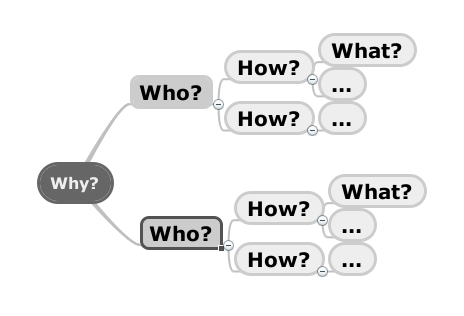
\includegraphics[scale=0.6]{images/impact_map.png}
	\caption{Carte d'impact}
	\label{impact_map}
\end{figure}

	
	\newpage
	\section{Proposition}
		-dire ce que je propose et pourquoi (pourquoi et pour quoi/qui, comment ça sera censé être utilisé, dans quel but) :
-> proposition d'une méthode de conception participative de JV thérapeutiques. Préciser les points importants de la conception, comme l'adaptation de la difficulté.
* propositions (théoriques) d'adaptation de de gameplay pour des NUI (m'inspirant de l'existant et des méthodes de rééduc)
	- parler ici de me la phase de veille / test, en testant le leap motion, des jeux sur Wii et Kinect PSMove, me permettant de faire des propositions plus pertinentes sur les controles.
* Cas pratique défini : travail sur l'équilibre (et lombalgie) et devices (kinect et wii)
*définition de la difficulté dans le jeu vidéo thérapeutique (ma position est que c'est différent des jeux classiques)
	
	\newpage
	\section{Réalisation}
	\subsection{Interface thérapeutique pour l'ajustement de la difficulté de serious games}	
\emph{Hammer \& Planks} est, dans sa version thérapeutique, un jeu permettant d'aider à récupérer des facultés motrices dans le cadre d'un accompagnement à la rééducation. Rappelons qu'il s'agit d'un shooter à défilement vertical dans lequel le joueur contrôle un bateau qu'il dirige avec des mouvements du corps. Le joueur doit éviter des obstacles, affronter divers ennemis et ramasser des bonus sur la mer. Tous ces objets possèdent des attributs qu'il est possible de modifier afin d'adapter le jeu aux besoins et aux capacités du patient. Ce fut mon travail durant la première partie de mon stage de permettre de modifier ces paramètres directement à partir d'une interface web contrôlée par le soignant menant la séance de thérapie.
\paragraph{}
Ce projet se divise en deux parties distinctes~:
\begin{enumerate}
	\item L'interface thérapeutique
	\item Le paramétrage des variables de jeu
\end{enumerate}

	\subsubsection*{Interface thérapeutique}
Celle-ci permet, à partir d'un terminal distinct, de choisir un jeu et de lancer une partie sur le terminal utilisé par le patient. Ce dernier sera équipé d'un périphérique de contrôle comme la caméra Kinect ou la wii board. A partir de cette interface, le soignant est en mesure de voir et de modifier l'ensemble des paramètres de jeu (en tout cas, le sous-ensemble considéré comme pertinent et effectivement envoyé à l'application). De plus, à la fin d'une partie, il sera capable de visualiser les données de la session de jeu, comme l'apparition d'évènements ou les zones que le joueur a réussi ou non à atteindre. Ces informations sont utiles pour mieux cibler les difficultés du patient et ajuster au mieux les prochaines séances. Cette partie du projet a été réalisée par Andy Camicci durant son stage chez NaturalPad entre Avril et Juin 2013.

\begin{figure}[htbp]
	\centering
%	\includegraphics[scale=]{images/interface_therapeutique_01.png}
	\caption{TODO Modification des valeurs du jeu dans l'interface thérapeutique}
	\label{interface_therapeutique_01}
\end{figure}

\begin{figure}[htbp]
	\centering
%	\includegraphics[scale=]{images/interface_therapeutique_02.png}
	\caption{TODO Visualisation des données de la partie.}
	\label{interface_therapeutique_02}
\end{figure}

	\subsubsection*{Maitriser la difficulté : le paramétrage des variables de jeu}
Cette partie consiste en l'extraction des paramètres de jeux et en la création d'un système permettant de créer, d'enregistrer et de transmettre des configurations de ces attributs à l'interface thérapeutique.

\paragraph{}
\emph{Hammer \& Planks} est développé avec le moteur de jeu Unity3d et les scripts codés avec le langage de programmation C\#. Comme nous l'avons dit, \emph{H\&P} possède de nombreux contenus contribuant à la richesse du gameplay et aux possibilités d'ajustement. Lors de mon arrivée au sein de NaturalPad, ces objets n'étaient cependant pas ajustables facilement : il fallait rechercher l'ensemble des objets dont on souhaitait modifier un paramètre, trouver les variables correspondant à ces paramètres puis les modifier soit directement dans le code soit par l'intermédiaire de l'éditeur d'Unity. La raison en est que les contraintes de développement du jeu n'ont pas permis de découpler ces informations.

\paragraph{}
Mon premier travail a donc été de découvrir le code et de rechercher toutes les variables dont on souhaiterait potentiellement vouloir modifier la valeur dans un contexte d'ajustement du jeu pour un exercice de rééducation. J'ai ensuite créé une classe spécifique permettant de regrouper conceptuellement les données modifiables. J'ai ainsi regroupé ces données dans des thèmes tels que \emph{réseau}, \emph{ennemis}, \emph{joueur}, \emph{contrôles} ou \emph{cosmétiques}.

\paragraph{}
En parallèle, j'ai aussi procédé au refactoring de l'ensemble des classes possédant ou utilisant un ou plusieurs attributs modifiables. L'intérêt était bien sur d'avoir un accès commun unique à ces valeurs, mais aussi et surtout que les valeurs puissent être modifiées de manière extérieure par l'interface thérapeutique. Par ailleurs, la modification de ces valeurs par l'interface devait être certaine et pérenne, afin que les modifications apportées soit effectivement prises en compte par l'application et donc modifier l'expérience de jeu en direct.

	\subsubsection*{Préparer l'évolution du jeu et de la séance}
Si permettre un ajustement en direct des propriétés du jeu par le soignant était une fonctionnalité que nous voulions impérativement mettre en place, celle-ci peut se révéler contraignante et répétitive si elle est utilisée seule. Nous voulions ainsi la possibilité de pouvoir enregistrer des configurations de paramètres, afin de pouvoir passer de l'une à l'autre aisément sans devoir faire chaque modification séparément. Par ailleurs, cela permet d'envisager beaucoup de possibilités comme la personnalisation de configurations pour des patients, l'adaptation aisée du jeu pour des besoins thérapeutiques différents ou encore l'automatisation d'une progression de la difficulté à l'aide de configuration prédéfinies.

\paragraph{}Afin d'utiliser des fichiers de configurations, il a fallu créer un système permettant de serialiser les données puis de les charger et de les lier à l'instance de jeu.\\
J'ai par ailleurs durant mon stage créer plusieurs fichiers de configuration permettant une évolution progressive de la difficulté dans le mode de jeu Survie de \emph{Hammer \& Planks}, pour sa version grand public.

	\subsubsection{Usage : tests, retours et intégrations}
Si le projet \emph{Hammer \& Planks} a été initié par une étudiante en ergothérapie, il est aussi et surtout développé en collaboration avec le pôle de rééducation du centre hospitalier de Lapeyronie à Montpellier. Comme nous l'avons dit, le projet a évolué et son champs d'action, en plus d'un travail sur l'équilibre, s'étend maintenant à de l'aide à la rééducation des membres supérieurs, du tronc et du bassin. Le travail d'équilibre, qu'il soit debout ou assis, s'effectue en utilisant la balance de la Wii, qui enregistre les changements du centre de gravité du joueur-patient pour contrôler le bateau. L'intégration d'un contrôle avec la Kinect permet au joueur d'utiliser d'autres mouvements de son corps. Il est ainsi possible d'utiliser son bras ou sa main pour diriger le bateau, ou les mouvements du tronc et du bassin que ce soit en position assise ou debout.

\paragraph{} Nous approchant d'une méthode de conception participative, nous avons ainsi réalisé plusieurs séances de tests avec des patients hémiplégiques et leurs thérapeutes. \\
Les premières choses marquantes sont la curiosité et l'enthousiaste général à la fois des patients et du personnel soignant. Peu d'entre eux connaissaient l'existence de jeux sérieux pour la santé, et dans le cas contraire, appréciaient particulièrement l'accent mis sur l'aspect vidéo-ludique de \emph{Hammer \& Planks}. Ce fut donc un premier point très positif pour l'équipe.

\paragraph{} 
Lors de la première séance de tests, nous avons ainsi eu de nombreux retours positifs portant sur la possibilité d'ajuster le jeu en direct, la visualisation des informations de la session de jeu ou encore le plaisir de jeu. Nous avons aussi eu de nombreuses remarques menant à l'ajout de fonctionnalités, notamment par le personnel.\\
Les remarques les plus fréquentes concernaient le visuel du jeu : les soignants craignaient que les graphismes soient trop riches et les effets trop complexes pour des patients hémiplégiques. L'effet visuel des mouvements de la mer fut notamment cité, et la différenciation entre bonus et obstacles (ennemis, projectiles et mines ennemies) jugée trop complexe.\\
Enfin, réaliser des tests pendant une demie-journée nous a aussi permis de juger notre travail de manière différente. Nous avons ainsi remarqué que nous faisions régulièrement voir systématiquement certains ajustements de paramètres, alors que certaines valeurs n'étaient jamais utilisées.

\paragraph{De l'importance des tests utilisateurs\\}Petite anecdote enfin, prouvant définitivement l'importance de réaliser des tests en conditions réelles. Lorsqu'on utilise le jeu avec la Kinect, le joueur doit lever la main afin d'être reconnu comme la personne joueuse parmi les possibles multiples personnes détectées par la caméra. Ce système fonctionnait parfaitement lors de nos test en interne. Or quand une patient hémiplégique a tenté de jouer, le système ne la reconnaissait pas. La raison en était que la patiente avait une hémiplégie du coté gauche et voulait donc jouer avec sa main gauche pour travailler sa rééducation. Or, le système était configuré pour ne détecter qu'une main droite... aucun membre de l'équipe n'étant gaucher, nous n'avions pas détecté ce grossier oubli ! L'erreur a bien sur depuis était corrigée.

	\paragraph{\emph{Intégration}\\}
	Forts de ces retours, nous avons ensuite classé les remarques qui nous été faites et celles que nous avons notées. Puis, nous avons discuté de la pertinence et de l'importance de chacune d'elle, ainsi que des différentes possibilités d'y répondre. \\
	Concernant la surcharge visuelle, pouvant poser des problèmes cognitifs à certains patients, surtout pour des personnes peu voir pas habituées aux jeux vidéo, nous avons mis en place la possibilité d'ajuster les paramètres visuels. Il est possible de modifier le contraste du jeu, la taille des éléments interactifs ou encore de supprimer les objets cosmétiques (requins, mouettes, brouillard, effet de la mer, etc.). Nous avons par ailleurs augmenté la taille des projectiles (ennemis et alliés) et ajouté un effet de trainée, les rendant beaucoup plus visibles.\\
	Concernant les bonus, jugés trop difficiles à ramasser, nous mis en place deux systèmes. Le premier est la possibilité de mettre un halo vert autour des différents bonus, les rendant bien plus visibles. Le second, est un mécanisme d'aimantage des bonus vers le bateau du joueur. Cette attraction, dont le rayon est ajustable dans les settings, permet de récupérer les bonus même si on ne passe pas directement dessus, ce qui est souvent difficile et frustrant pour le joueur.\\
Concernant les paramètres enfin, nous modifié les valeurs par défaut de certains et ajuster les bornes min et max des plages de valeurs.

		
	\paragraph{} Nous avons ensuite réalisé une nouvelle séance de tests du jeu intégrant ces modifications. C'est avec plaisir que nous avons constaté que les réponses apportées étaient pertinentes et plaisaient à nos testeurs. Ce fut aussi l'occasion d'avoir de nouveaux retours et de continuer notre processus de conception participative.
	
\paragraph{montrer un aperçu des valeurs modifiables?} et leur utilité d'un point de vue
ajustement et rééduc. Et peut être aussi des images sur le thème "avant/après" pour montrer l'évolution et l'intéret des test en situation.

	\subsubsection{Conclusion}
	Cette expérience et ce travail sur \emph{Hammer \& Planks} m'ont permis de vérifier l'intérêt et la réelle pertinence de jeux sérieux pour la rééducation. Par ailleurs, l'intégration d'un nouveau périphérique, la Kinect, débloquant de nouveaux gameplay avec un système de jeu identique, m'a confirmé l'importance du moyen de contrôle à la fois sur le gameplay mais aussi et surtout sur la richesse des applications thérapeutiques qui en découle. Enfin, les critiques des soignants et des patients au cours des deux séances de tests m'ont assuré de l'importance et du réel intérêt de pouvoir ajuster manuellement les variables de jeux directement pendant la séance. C'est à la fois très gratifiant pour notre travail et très encourageant pour les possibilités en terme de réhabilitation.
	
\paragraph{}
Cependant, un seul jeu, aussi ajustable soit il, ne peut suffire à répondre à tous les besoins et cas d'utilisation. Il y a trois aspects~:
\begin{enumerate}
	\item le cœur du jeu, qui décrit ses lois, objectifs et règles de fonctionnement. Il est propre au jeu (ou à un type de jeu) et non modifiable.
	\item les variables ajustables, qui ne modifient pas les règles mais définissent entre autres la difficulté.
	\item le gameplay, induit par les deux premiers points ainsi que par les périphériques et méthodes de contrôle utilisés. En général, ces derniers sont pris en compte dès l'établissement du coeur du jeu, certaines associations étant incompatibles.
\end{enumerate}
\paragraph{}
Il est possible de modifier l'expérience de jeu en modifiant la valeur des variables ajustables : c'est ce que nous proposons à l'aide de notre interface thérapeutique. Il est aussi possible d'explorer un gameplay a priori identique avec des contrôleurs différents, rendant ainsi à la fois l'expérience de jeu et les mouvements induits différents.
\\Cependant, même ainsi, un jeu vidéo avec un coregame propre finit par montrer ses limites en terme d'adaptation, et il est alors nécessaire de proposer d'autres types de jeux vidéo si l'on veut explorer de nouvelles pistes de rééducation.\\
Pour cette raison, toujours dans l'idée d'une adaptation de la difficulté, la suite logique était de proposer une méthode permettant d'aider à la conception de jeux sérieux thérapeutiques.

\paragraph{}
\subsection{Conception}
	*conception participative avec Arnaud 
		-impact mapping, carte d'empathie et scénarios d'usage et storyboard
	
	-travail avec les thérapeutes
	-répondre aux objectifs thérapeutique par un gamedesign
		- hammer \& Planks et l'équilibre (voir rapport d'anais)
		- classement des objectifs thérapeutique, carte d'impact
	-ajustement de la difficulté et lien avec la thérapie : impact des paramètres en terme de difficulté (équilibre et dos?)
	
	-proposition de controle naturels pour des jeux pour une utilisation thérapeutiques
	
	\newpage
	\section{Perspectives}
		hammer and planks : (paramètres de difficulté, groupe d'ennemis)\newline
	
	-avoir une information de profil pour cibler la difficulté -> nourrir un systeme de recommandation\\
	-ajustement dynamique de la difficulté selon le profil/résultats du joueur\newline
	-étendre le domaine de la méthodologie à d'autre pathologies et matériels\newline
	-éprouver les propositions de méthodo, sur un cas concret et complet\newline
	-permettre un paramétrage par objectifs non par paramètres permettant de faciliter l'utilisation de la plateforme et des jeux par les thérapeutes \newline
	- Le pb c'est que j'ai rien qui dise clairement "pour tel exercice/objectif, fais plutot ce type de jeu avec tels contrôles. Du coup, est-ce que ca pourrait pas être une forme de perspective? disant que ça nécessiterait du travail et serait moins parfait qu'un truc personnalisé, mais ca permettrait de gagner du temps tout en étant mieux que ce qui existe actuellement

	
	\newpage
	\section{Conclusion}
	Globalement, ce stage était sur le thème des échanges et au carrefour entre le monde informatique et le monde médical. Nous avons vu comment allier l'expérience d'une société dans le développement de jeux vidéo, à la connaissance et l'expertise de professionnels de la santé, pour proposer un jeu sérieux efficace et apprécié des joueurs.

\paragraph{}
Ce stage de fin d'étude fut aussi l'occasion de vérifier sur une période longue de six mois que mon niveau de compétence et mon autonomie de travail étaient suffisants. Si j'avais déjà réalisé un stage de deux mois chez NaturalPad, l'accent avait alors était mis sur le développement et l'acquisition de connaissances web. J'avais à cette époque parlé de mon intérêt pour les échanges avec des professionnels d'autres corps de métier. En ayant reparlé avec Antoine Seilles, nous avons axé mon travail de stage vers de la conception avec des thérapeutes. Cela m'a montré l'importance de la communication dans une équipe et nous a permis de trouver un sujet de stage en accord avec nos besoins et envies respectifs.

\paragraph{}
Durant ce stage, j'ai donc participé au développement du serious game Hammer \& Planks, et ma connaissance du moteur de Unity3d fut un atout. J'ai travaillé aussi bien pour sa version grand public, enrichissant mes compétences en game design, que sur la version thérapeutique d'aide à la rééducation motrice. Celle-ci me permit de tester et mettre en application un système d'ajustement des paramètres du jeu, dans le but d'agir sur la difficulté ou l'adaptation du jeu aux capacités du joueur-patient. Cette adaptation se fait au moyen d'une interface web thérapeutique permettant de modifier la valeurs des variables du jeu ou des paramètres de réglage des contrôles par exemple.

\paragraph{}
Nous avons aussi réalisé des séances de tests avec des thérapeutes et des patients représentant les utilisateurs futurs du jeu. Cela m'a permis de confronter mon travail aux critiques et appréciations de personnes complètement étrangères au travail de développement. Ce fut très constructif à la fois pour mieux comprendre les joueurs, mais aussi d'un point de vue humain. Voir une jeune fille de moins de 20 ans, hémiplégique, et se régalant de jouer à Hammer \& Planks, fut réellement touchant. De la même manière, s'entendre féliciter à plusieurs reprises par un homme de plus de 70 ans en disant que grâce à notre travail il trouvait enfin amusant une activité à l'hôpital, est en soi une récompense.

\paragraph{} C'est d'ailleurs l'aspect positif que je suis venu chercher et trouver en venant travailler chez NaturalPad. Je souhaitais utiliser mes connaissances et compétences informatiques dans un contexte différent que le développement d'applications classiques, et basé sur les échanges humains. NaturalPad est une société dont les valeurs correspondent aux miennes, que ce soit dans les pratiques ou les solutions développées.

\paragraph{} Cela m'amène au point suivant, puisque, comme nous l'avons vu, NaturalPad est une société innovante se positionnant sur le marché des serious games. En correspondance avec ma formation, elle m'a permis d'étendre très largement mes connaissances à ce sujet en m'offrant la possibilité d'effectuer un travail de recherche et d'état de l'art. J'ai ainsi beaucoup appris sur les serious games en général, les théories d'apprentissage ou encore la réhabilitation. Ces recherches me seront particulièrement utiles tout d'abord au niveau des connaissances théoriques acquises, mais aussi au niveau de la démarche de travail effectuée. Je souhaite ainsi poursuivre ce type de travail au moyen d'une thèse, sur les serious games ou la difficulté notamment. 

\paragraph{} J'ai aussi proposé plusieurs outils d'aide à la conception ainsi qu'une méthodologie de conception  de serious games pour la santé. Ces travaux m'ont permis d'explorer différentes pistes, de communiquer avec des chercheurs et des thérapeutes et 
leur proposer ces solutions. De nombreuses perspectives sont possibles pour faire évoluer ces outils ou valider la méthodologie, mais les résultats acquis durant le stage sont prometteurs.

\paragraph{} Durant mon stage, l'équipe de NaturalPad a su me faire confiance en me laissant autonomie, prises de décisions et responsabilités. Après avoir assisté à plusieurs séances de conception participative, Antoine Seilles a jugé que j'étais en mesure de mener ma propre séance en m'invitant à diriger une séance au centre hospitalier d'Alès Cévennes (CHAC). \\
J'ai aussi rencontré de nombreux professionnels de la santé de ma propre initiative, ergothérapeutes ou kinésithérapeutes, en fonction des besoins, contribuant à faire évoluer mon travail dans la bonne direction.

\paragraph{}
Enfin, ce stage fut globalement une très bonne expérience. J'ai beaucoup appris technologiquement grâce aux connaissances et aux partages de mes collègues. J'ai aussi passé six mois de réelle bonne humeur, chacun étant libre de s'exprimer et de proposer.
Dans cette optique, l'équipe a par ailleurs réalisé deux game jam d'une semaine durant la période où j'y ai travaillé. Une game jam consiste en la création d'un jeu sur une période courte. Ce fut l'occasion pour chacun de faire jouer son imagination, de mettre en place ses idées et de changer de contexte de travail d'une manière des plus agréables. Les mini-jeux réalisés nous plaisent d'ailleurs particulièrement, et je recommande à tout fan de jeux vidéo de se lancer dans cette expérience.
	
	\newpage
	\printglossaries
%	\addcontentsline{toc}{chapter}{Glossary}

	\newpage
	\bibliography{rapport}

\newpage
\part{Annexes} \appendix
	%\section{Les différents types 'classiques' de Jeux Vidéo} \label{types_jeux}
	%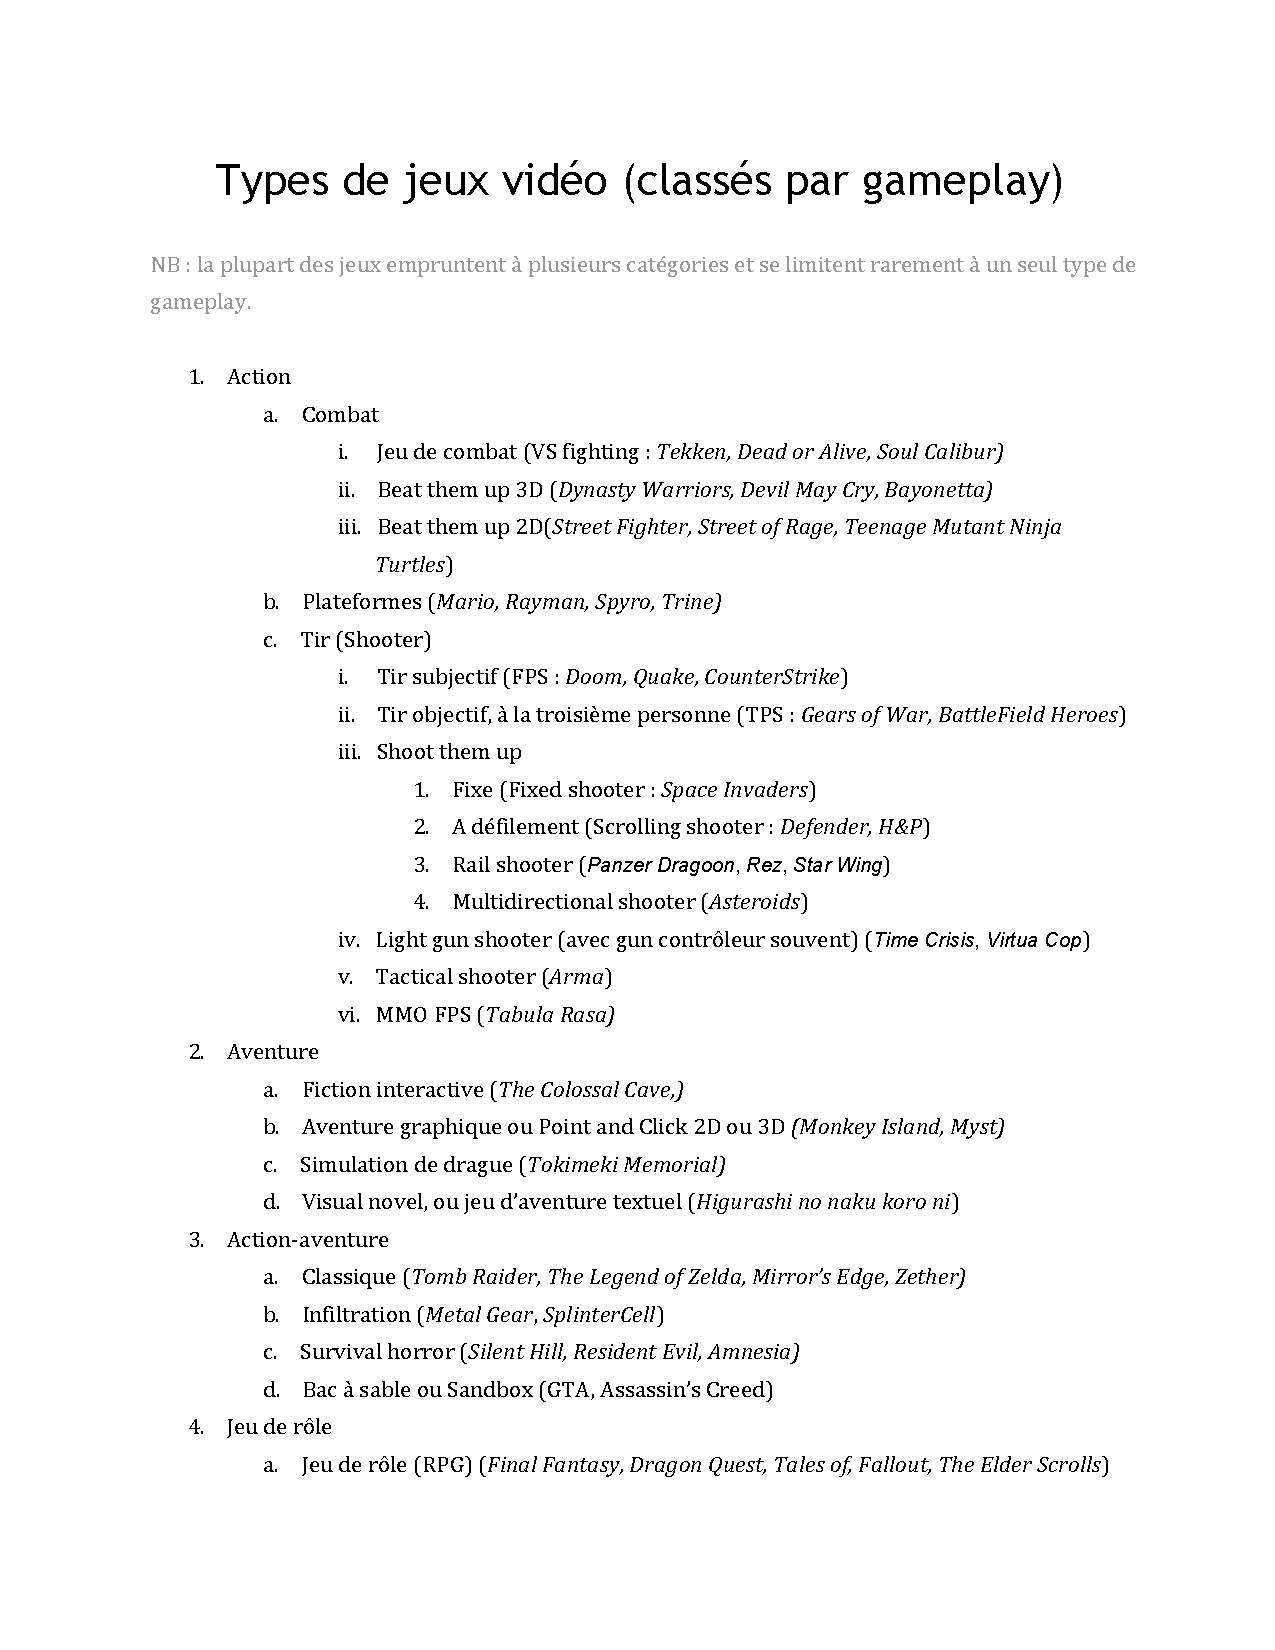
\includepdf[pages=-]{chapters/types_jeux_video} %inclusion de toutes les pages du pdf
	
	%\section{Esquisse d'énumération des éléments d'un jeu et association avec les théories cognitives et comportementales} \label{matching}
	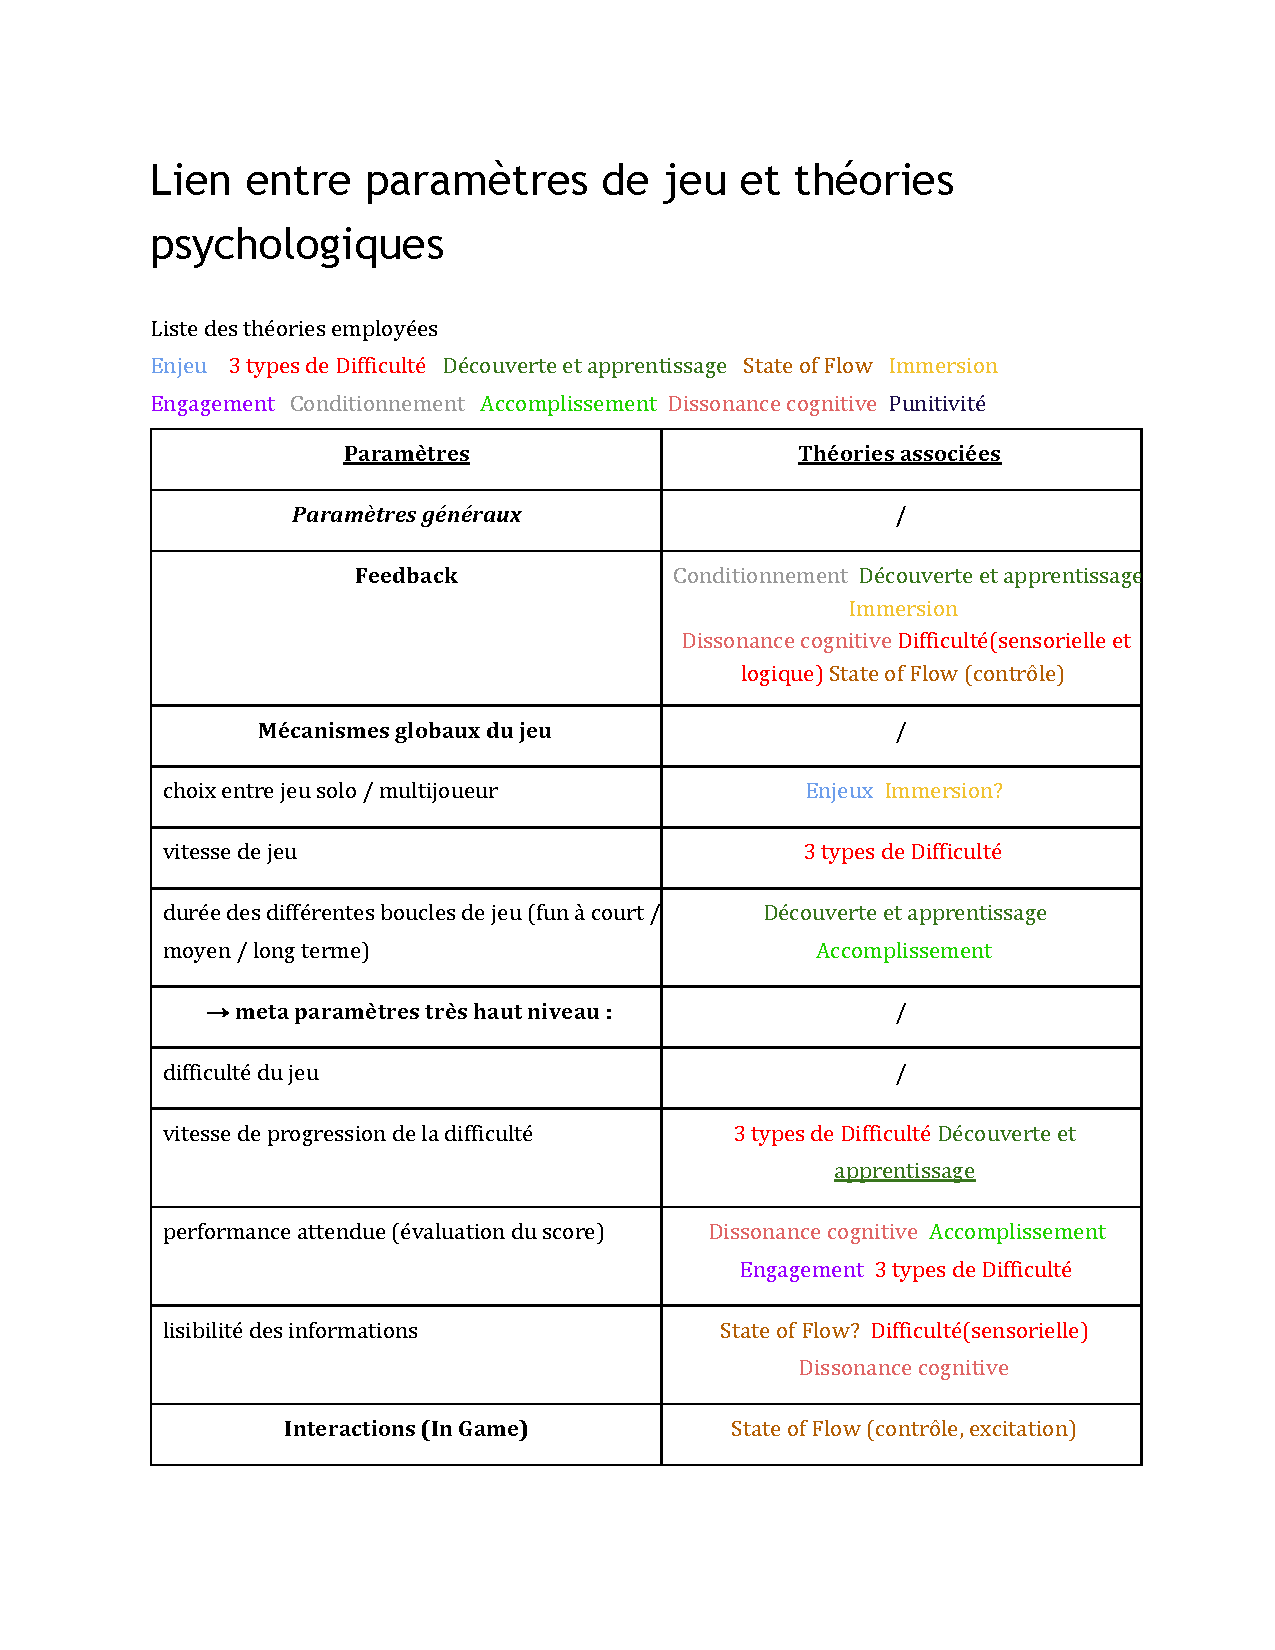
\includepdf[pages=-]{chapters/matching_objets_et_theories_v1}
	
	%\section{Proposition de contrôles naturels pour des jeux existants} \label{propositions_controles}
	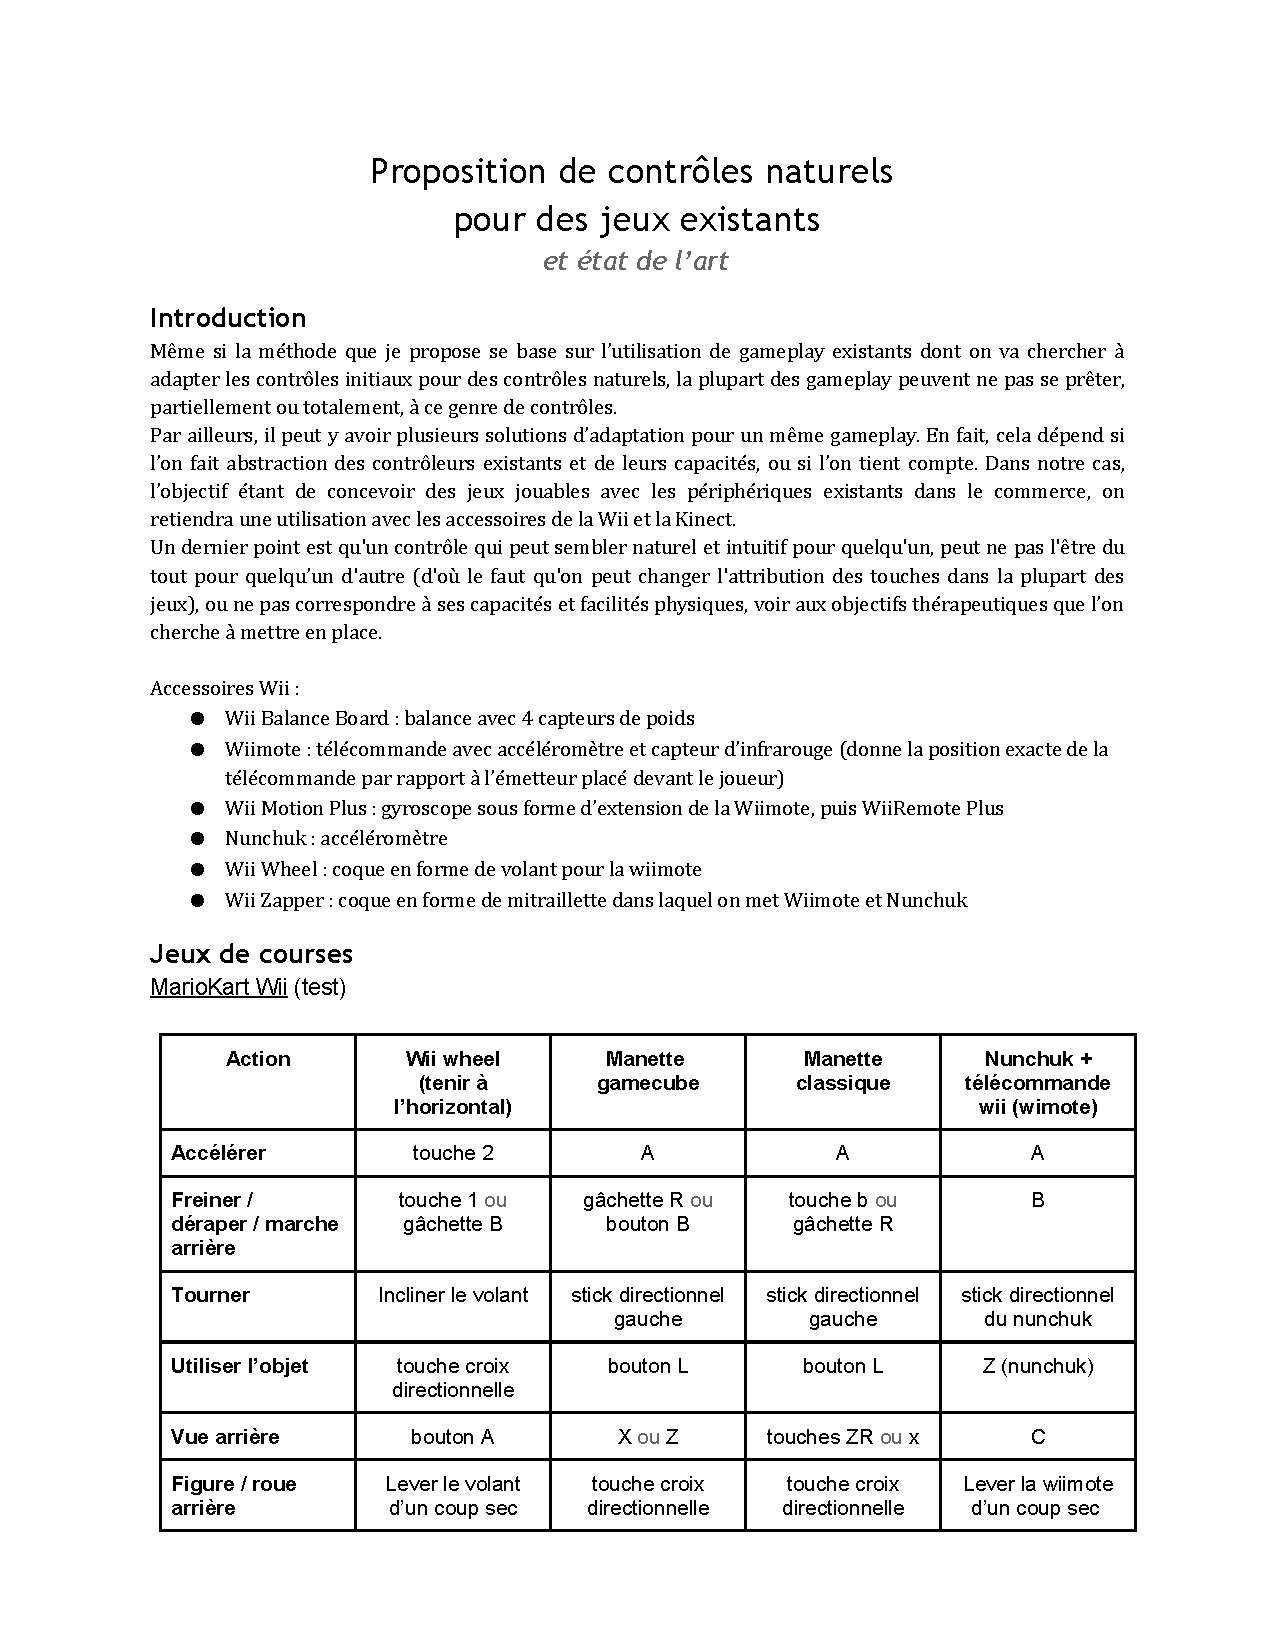
\includepdf[pages=-]{chapters/propositions_controles}

	
%Voir dans quelle mesure il peut être intéressant de mettre mes comptes rendus d'entretien. Dans des annexes séparées éventuellement.
\end{document}